%!TEX TS-program = xelatex
%!TEX encoding = UTF-8 Unicode

\documentclass{papon_thesis}
\usepackage{todonotes}
%\usepackage[]{showkeys}
\makeglossaries

\begin{document}
\watermark {DRAFT COPY ONLY}
\newacronym{vos}{VOS}{Video Object Segmentation}
\newacronym{pdf}{PDF}{Probability Distribution Function}
\newacronym{mtt}{MTT}{Multi-Target Tracking}
\newacronym{ai}{AI}{Artificial Intelligence}
\newacronym{mtvt}{MTVT}{Multi-target visual tracking}
\newacronym{sbf}{SBF}{Sequential Bayesian Filtering}
\newacronym{msvs}{MSVS}{Mean-shift video segmentation}
\newacronym{mhvs}{MHVS}{Multiple hypothesis video segmentation}
\newacronym{pva}{PVA}{Propagation, validation, and aggregation}

% the front matter
% some details about the thesis
\title{Perceptual Segmentation of Visual Streams by Tracking of Objects and Parts}
\author{J\'{e}r\'{e}mie Papon}
\advisor{Prof. Dr. Florentin W\"org\"otter}

% about the degree
\degree{Doctor of Philosophy}
\field{Computer Science}
\degreeyear{2014}
\degreemonth{March}

% about the university
\department{Faculty of Natural Sciences and Mathematics}
\university{Georg-August-Universit\"{a}t G\"{o}ttingen}
\universitycity{G\"{o}ttingen}
\universitystate{Germany}

\makegermantitle
\cleardoublepage
\maketitle
\cleardoublepage
\referentpage
\newpage \thispagestyle{empty} \vspace*{\fill}
 
\noindent 

\textsc{  }
\begin{flushleft}
The canonical version of this document is the electronic copy maintained in the Github repository by the author. At this time, it is maintained at:\
\end{flushleft}
\begin{center} \url{https://github.com/jpapon/papon_thesis/thesis.pdf} \\ \end{center}

\begin{flushleft}
This work is licensed under a Creative Commons Attribution-NonCommercial 4.0 International License. The full terms of the license can be viewed online at:\
\end{flushleft}
\begin{center} \url{http://creativecommons.org/licenses/by-nc/4.0/} \\ \end{center}

\begin{flushleft}
Much of the code created as a result of the research in this thesis is freely available under a BSD license as part of the Point Cloud Library:\
\end{flushleft}
\begin{center} \url{http://www.pointclouds.org/} \\ \end{center}


\begin{flushleft}
The code for the Oculus Vision System (see Appendix \ref{chap:Oculus}) created as part of this thesis is freely available under GPLv3:\
\end{flushleft}
\begin{center} \url{https://launchpad.net/oculus} \\ \end{center}

\vspace{20pt}
\begin{center} For other usage, contact \url{jpapon@gmail.com}. \end{center}
\vspace{40pt}

\begin{center}
\begin{textsc}
\copyright~\textit{2014 \hspace{3pt}~- \theauthor} \\ 
\noindent All rights reserved.
\end{textsc}
\end{center}


\begingroup
\let\cleardoublepagecopy\cleardoublepage
\let\cleardoublepage\clearpage
\abstractpage
\tableofcontents
\listoffigures
\listoftables
\printglossary[type=\acronymtype,title=List of Acronyms,toctitle=Terms and Abbreviations]

\noindent
\begin{flushright}
\huge List of Related Publications
\end{flushright} 
\vspace{50pt} 

%The work described in this thesis has appeared in the following publications: \\
%\vspace{24pt} 
\hangindent=1.5cm \textbf{Papon, J.};  Wörgötter, F., ``{Spatially Stratified Correspondence Sampling for Real-Time Point Cloud Tracking,}'' \emph{Applications of Computer Vision (WACV), 2015 IEEE International Conference on}, Jan. 2015. \\
\vspace{6pt}

\hangindent=1.5cm \textbf{Papon, J.};  Kulvicius, T.; Aksoy, E.; Wörgötter, F., ``\href{http://www.dpi.physik.uni-goettingen.de/cns/uploads_bibtexmodule/PDF/paponkulviciusaksoy2013.pdf}{Point Cloud Video Object Segmentation using a Persistent Supervoxel World-Model,}'' \emph{Intelligent Robots and Systems (IROS), 2013 IEEE/RSJ International Conference on}, Nov. 2013. \\
\vspace{6pt}

\hangindent=1.5cm \textbf{Papon, J.};  Abramov, A.; Schoeler, M.; Wörgötter, F., ``\href{http://www.cv-foundation.org/openaccess/content_cvpr_2013/papers/Papon_Voxel_Cloud_Connectivity_2013_CVPR_paper.pdf}{Voxel Cloud Connectivity Segmentation - Supervoxels for Point Clouds,}'' \emph{Computer Vision and Pattern Recognition (CVPR) 2013}, June 2013. \\
\vspace{6pt}

\hangindent=1.5cm \textbf{Papon, J.};  Abramov, A.; Wörgötter, F., ``\href{http://dx.doi.org/10.1007/978-3-642-33885-4_24}{Occlusion Handling in Video Segmentation via Predictive Feedback,}'' \emph{European Conference on Computer Vision (ECCV) 2012}. Workshops and Demonstrations, Lecture Notes in Computer Science Volume 7585, 2012, pp 233-242. \\
\vspace{6pt}

\hangindent=1.5cm \textbf{Papon, J.};  Abramov, A.; Aksoy, E.; Wörgötter, F., ``\href{http://dx.doi.org/10.1109/WACV.2012.6163002}{A modular system architecture for online parallel vision pipelines,}'' \emph{Applications of Computer Vision (WACV) 2012}, pp.361-368, Jan. 2012. \\
\vspace{6pt}

\hangindent=1.5cm Stein, S.; Schoeler, M.; \textbf{Papon, J.};  Wörgötter, F., ``\href{http://www.cv-foundation.org/openaccess/content_cvpr_2014/html/Stein_Object_Partitioning_using_2014_CVPR_paper.html}{Object Partitioning using Local Convexity,}'' \emph{Computer Vision and Pattern Recognition (CVPR) 2014}, June 2014. \\
\vspace{6pt}

\hangindent=1.5cm Stein, S.;  Wörgötter, F.; Schoeler, M.; \textbf{Papon, J.}; Kulvicius, T., ``\href{http://www.dpi.physik.uni-goettingen.de/cns/modules/BibtexModule/uploads/PDF/steinwoergoetterschoeler2014.pdf}{Convexity Based Object Partitioning For Robot Applications,}'' \emph{Robotics and Automation (ICRA), 2014 IEEE/RSJ International Conference on}, June 2014. \\
\vspace{6pt}

\hangindent=1.5cm Schlette, C.; Buch, A.; Aksoy, E.; Steil, T.; \textbf{Papon, J.}; Savarimuthu, T.R.; Wörgötter, F.; Krüger, N.; Roßmann, J., ``\href{http://link.springer.com/article/10.1007/s11740-014-0552-0}{A new benchmark for pose estimation with ground truth from virtual reality,}'' \emph{Production Engineering}, May 2014. \\
\vspace{6pt}

\hangindent=1.5cm Aein, M.J.;  Aksoy, E.; Tamosuinaite, M.; \textbf{Papon, J.}; Ude, A.; Wörgötter, F., ``\href{http://ieeexplore.ieee.org/xpls/abs_all.jsp?arnumber=6697011&tag=1}{
Toward a library of manipulation actions based on semantic object-action relations,}'' \emph{Intelligent Robots and Systems (IROS), 2013 IEEE/RSJ International Conference on}, Nov. 2013.\\
\vspace{6pt}

\hangindent=1.5cm Abramov, A.; Pauwels, K.; \textbf{Papon, J.}; Wörgötter, F.; Dellen, B., ``\href{http://dx.doi.org/10.1109/WACV.2012.6163000}{Depth-supported real-time video segmentation with the Kinect,}'' \emph{Applications of Computer Vision (WACV) 2012}, Jan. 2012.\\
\vspace{300pt}

The research leading to this thesis was supported with funding from the European Community's Seventh Framework Programme FP7/2007-2013 (Specific Programme Cooperation, Theme 3, Information and Communication Technologies) under grant agreement no. 270273, Xperience and grant agreement no. 269959, IntellAct.

 

\endgroup
\let\cleardoublepage\cleardoublepagecopy
%\dedicationpage
\acknowledgments


\onehalfspacing
\mainmatter
% include each chapter...
\begin{savequote}[75mm]
Some Quote.
\qauthor{Quoteauthor Lastname}
\end{savequote}

%For an example of a full page figure, see Fig.~\ref{fig:myFullPageFigure}.

\chapter{Introduction}
\newthought{There's something to be said} for having a good opening line.
\section{Problem Definition and Motivation}
\subsection{The Image Segmentation Problem}
\subsection{The Tracking Problem}
Multi-target visual tracking (MTVT) and 6DoF pose estimation are crucial challenges for many applications such as visual surveillance, action recognition, and robotic imitation learning. In many such functions, visual tracking serves as the precursor to all further high-level inference, making robust tracking fundamental to the success of a large variety of intelligent systems. Related to the problem of visual tracking is segmentation, the task of grouping observations according to the entities which they contain. Video object segmentation (VOS) attempts to cluster pixels of video frames into segments which are both spatially and temporally coherent. While generally similar to MTVT, VOS goes a step beyond localizing tracked objects, in that it makes an association decision for each observed pixel; in addition to estimating overall state, it must re-estimate spatial extent every frame. In both VOS and MTVT there are two chief challenges that must be addressed: first, the data association problem, whereby 
noisy observations must be associated with the proper targets, and secondly, the occlusion problem, in which targets may become partially or fully obscured for a number of observations.

\subsection{Segmentation In Sequential Frames}
Video segmentation has the potential to be more accurate than single image segmentation, as it can take advantage of the temporal coherence of objects in space to infer information about the objects in a scene. Unfortunately, the addition of the temporal domain brings along new challenges as well; for instance that pixels which should be grouped across time may not be continuously visible, as in the case of partial or full occlusions. Additionally, the added dimension increases the computational complexity of the problem, making accurate segmentation a costly procedure. Temporal information also increases the exposure of the algorithm to noise, as each image frame is a separate noisy measurement. This adds a large amount of uncertainty to the problem, since measured values (i.e., of color) for an object can show significant variation over time. 

While MTVT and VOS are clearly related, they traditionally have been considered separate areas of research. In this work, we unify them by taking a mature tracking approach, particle filtering, and apply it to tracking supervoxels (3d segments) from a recent 3d segmentation technique \cite{VCCS_Papon_2013}, Voxel Cloud Connectivity Segmentation (VCCS). To make this possible, we extend the concept of VCCS to dynamic scenes by maintaining a world-octree supervoxel model which lets objects persist indefinitely through occlusions. Additionally, we use a novel global energy function to associate observations to predictions, and thereby extract accurate object segmentations (even for fully occluded objects) from tracker predictions.

\subsection{Perception as Accumulation of a 3D World Model}

\section{State of the Art}
\subsection{Segmentation and Superpixels}
Segmentation of scenes into objects remains one of the most challenging topics of computer vision despite decades of research. To address this, recent methods often use hierarchies which create a rank order that build bottom-up from small localized superpixels to large-scale regions \cite{Ren:ICCV2003,Ahuja:CVPR2008,Arbelaez:PAMI2011}. As an alternative, researchers have also pursued strictly top-down approaches. These began with coarse segmentations using multiscale sliding window detectors \cite{ViolaJones:IJCV2004}, later progressing to finer grained segmentations and detections based on object parts \cite{Felzenswalb:PAMI2010, Bourdev:ICCV2009}. These two avenues of research led naturally to methods which {\em combine} bottom-up hierarchy building with top-down object- and part-detectors \cite{Arbelaez:CVPR2012, Silberman:ECCV12, Gupta:CVPR2013}. While these approaches have yielded quite good results even on complex, varied data sets, they have lost much of the generality of learning-free approaches. In general the most powerful methods to-date use trained classifiers for segmentation \cite{Silberman:ECCV12, Gupta:CVPR2013}. This means they cannot be applied to arbitrary unknown scenes without being retrained, requiring the acquisition of a new data-set tailored to each test environment.

In this work we investigate model- and learning-free bottom-up segmentation of 3D point clouds captured with RGB-D cameras. In particular, we focus on the partitioning of cluttered scenes into basic {\em object parts} without the need for training data. As inspiration for a general rule for breaking scenes into elemental parts, we look to psychophysical studies, mostly performed on 2D images, which suggest that the transition between convex and concave image parts might be indicative of the separation between objects and/or their parts \cite{Koenderink1984,Vaina1990,Rosin2000,Matsuno2007,Cate2010,Bertamini2013}. While this feature has been used in machine vision to some degree \cite{Hoffman1987,Moosmann2009,Richtsfeld:IROS12,Ritter2012,Karpathy2013} success has remained limited and more recent studies were forced to combine this feature with additional, often very complex feature constellations to achieve good scene partitioning \cite{Richtsfeld:IROS12,Ritter2012,Karpathy2013}. It, thus, appears that direct transfer from 2D to 3D of the conventional, geometrically-defined convex-concave transition criterion shown in Fig.~\ref{fig:details}~A is not possible for achieving good 3D-segmentation. This puzzling observation can best be understood by ways of an example.

\subsection{Multi-Target Tracking}
Bayesian predictive filtering is a broad, well-established field in target tracking applications \cite{TrackingMultipleParticleFiltering,MonteCarloMTT,SequentialMonteCarloMultitargetFiltering}. While effective for tracking, these methods generally depend on fixed models with a small dimensional state-space, and are unable to deal with the high-dimensionality of VOS. Nevertheless, there exist a few methods which attempt to apply tracking methodologies to the VOS problem. A recent method \cite{TrackingOcclusionsGraphCuts} uses graph cuts to extract segmentations, and a dynamical model to form predictions which guide successive segmentations. Unfortunately, this method formally models visible and occluded parts of the tracked objects, and so does not scale well with an increasing number of objects, and thus is better suited to extracting the silhouettes of a few objects than performing a full segmentation. Other methods, such as \cite{LayeredGraphicalModels}, are severely limited in that they require pre-
computed models which are calibrated to a ground plane in order to resolve occlusions. The previously discussed work of Brendel and Todorovic  \cite{SegTrackRegions} also combines tracking and segmentation, but as mentioned earlier, it is an off-line method (performing smoothing rather than filtering) and thus cannot be used in many applications.

While MTVT remains an unsolved problem, single target visual tracking (STVT) is a fairly well-studied problem, with many mature approaches \cite{RobustTrackingBabenko, StructuredSparseRepresentation}. Additionally, recent work has progressed in estimating pose (in addition to tracks) for single targets, for example \cite{6DOFTracking} uses a particle filter to track 6-DoF pose of arbitrary objects in point clouds. Recent work in MTVT~\cite{MultiObjectTracking} successfully tracks multiple objects using a segmentation and association approach and adaptive 3D appearance models, but is limited by the need to align model point clouds to the observed data every frame. This precludes it from handling occlusions, as once a target is no longer observed, its track must be terminated.

\subsection{Video Object Segmentation}
There are many existing video object segmentation (VOS) methods, which can be classified based on three parameters; whether they are on- or off-line, whether they are dense or sparse, and whether or not they are supervised. We can reduce the comparison-space of related work by comparing only with algorithms which have the same three parameters as this work - on-line processing (the algorithm may only use past data), dense segmentation (every pixel is assigned to a spatio-temporal cluster), and unsupervised operation. Four state-of-the-art segmentation algorithms meet these requirements: Mean-shift video segmentation (MSVS) \cite{MSVS}, Multiple hypothesis video segmentation (MHVS) from superpixel flows \cite{MHVS}, Propagation, validation, and aggregation (PVA) of a preceding graph \cite{PropValAgg}, and Matching images under unstable segmentations \cite{MatchingUnstable}.  Of these methods, none are able to handle full occlusions; in fact only MHVS considers occlusions, and it is only able to handle partial 
occlusions for a few frames, and does not consider full occlusions. Even state of the art off-line methods such as that of Brendel and Todorovic \cite{SegTrackRegions} only handle partial occlusions, claiming that ``complete occlusions ... require higher-level reasoning''.  

Multiple hypothesis video segmentation (MHVS) from superpixel flows \cite{MHVS} provides dense online unsupervised video segmentations, but is only able to handle partial occlusions for a few frames, and does not consider full occlusions. There also has been much recent work in VOS specifically addressing the problem of segmenting foreground from background \cite{MWCwMC,GC_SURF}. While these works have been to shown to perform very well in their task, they only solve the single target case, as they do not need to resolve the multiple association problem.

In \cite{TrackingOcclusionsGraphCuts} Papadakis and Bugeau use a dynamical model to guide successive segmentations, along with an energy function minimized using graph cuts to solve the label association problem. They formally model visible and occluded regions of tracked objects, tracking them as distinct parts. While they do consider occlusions, they do not maintain a world model, and as such their methodology must fail under complete occlusions.

\section{Outline and Contributions}



%% Requires fltpage2 package
%%
% \begin{FPfigure}
% \includegraphics[width=\textwidth]{figures/fullpage}
% \caption[Short figure name.]{This is a full page figure using the FPfigure command. It takes up the whole page and the caption appears on the preceding page. Its useful for large figures. Harvard's rules about full page figures are tricky, but you don't have to worry about it because we took care of it for you. For example, the full figure is supposed to have a title in the same style as the caption but without the actual caption. The caption is supposed to appear alone on the preceding page with no other text. You do't have to worry about any of that. We have modified the fltpage package to make it work. This is a lengthy caption and it clearly would not fit on the same page as the figure. Note that you should only use the FPfigure command in instances where the figure really is too large. If the figure is small enough to fit by the caption than it does not produce the desired effect. Good luck with your thesis. I have to keep writing this to make the caption really long. LaTex is a lot of fun. You will enjoy working with it. Good luck on your post doctoral life! I am looking forward to mine. \label{fig:myFullPageFigure}}
% \end{FPfigure}
% \afterpage{\clearpage}

\cleardoublepage
\cleardoublepage
\begin{savequote}[75mm]
Some Quote.
\qauthor{Quoteauthor Lastname}
\end{savequote}

%For an example of a full page figure, see Fig.~\ref{fig:myFullPageFigure}.

\chapter{Video Segmentation by Relaxation of Tracked Masks}
\label{Chap:VideoSegRelaxation}
\lettrine[lines=3, loversize=0.3]{\textcolor{DarkBlue}I}{n the beginning}, 3D data, especially video data, was not readily available. As such, researchers were forced to make due with strictly 2D video, which is inherently ambiguous in many situations. In particular, partial and full occlusions are particularly vexing problems in 2D video - not least because understanding of 2D video is so easy for humans, yet so difficult to interpret algorithmically. Indeed, knowledge of object permanence, that is, the understanding of how to correctly interpret occlusions, is something that humans acquire very early on in their lives \cite{ObjectPermanence}, but has yet to be successfully implemented in a fully automated \gls{vos} system. Even after decades of research, state-of-the-art methods still have trouble correctly resolving partial occlusions, and typically fail completely after even the briefest of complete occlusions.

In this Chapter, we shall present our attempts towards resolving the object permanence problem with 2D data, as well as advance color-based \gls{vos} in general. In particular, we seek to overcome two of the main drawbacks of the color-based video segmentation method developed by Abramov et al. \cite{Abramov_RealtimeSegmentation} (and indeed, of color-based \gls{vos} in general). The first of these is the correct tracking of objects through partial and full occlusions, which we proposed to solve using a layering of deformable object masks that are allowed to interact and compete for ``ownership'' of pixels. The second is to allow for object identities to be maintained through sudden and/or fast movements - something that was not possible due to the core assumptions of the algorithm. To correct for this, we tracked the masks with a set of particle filters, a class of Bayesian predictive filters which are well known for their ability to handle difficult trajectories \cite{TrackingMultipleParticleFiltering,MonteCarloMTT,SequentialMonteCarloMultitargetFiltering}.

The underlying principle guiding the proposed algorithm is to use predictions from Bayesian filtering to inform segmentation of higher-level temporal object correspondences. It is well known that sequential Bayesian estimation methods perform well in difficult tracking scenarios \cite{Doucet2001}, and, under the Markov assumption, are computationally less demanding than video segmentation techniques such as MHVS \cite{MHVS}, which consider many prior frames. Particle filtering is one such method which has been shown to approximate the optimal tracking solution well, even in complex multi-target scenarios with strong nonlinearities \cite{TrackingMultipleParticleFiltering,MonteCarloMTT,SequentialMonteCarloMultitargetFiltering}. 

\section{Overview of the Algorithm}
\label{sec:Overview}
Before proceeding to discuss elements in detail, we shall first give a brief overview of the algorithm (depicted in Figure \ref{fig:AlgorithmFlow}). We begin by performing an initial segmentation (using any method) on the first frame $\mathbf{F}_{t_0}$ to generate an initial set of labels $\mathbf{S}_{t_0}$. An initial set of particles is generated for each label, and color histogram features are computed for each particle (as in \cite{ColorBasedProbabilisticTracking}). Thus each object $k$ at initial time $t_0$ is specified by a set of $N_k$ particles $\mathbf{X}^{k,1:N_k}_{t_0}$, each of which contains a representation of the object, specified by a pixel existence map $\mathbf{M}$, a reference color histogram $\mathit{\hat{q}}$, a position shift vector $\mathbf{p_{t_0}}$, and a velocity vector $\mathbf{v_{t_0}}$.

\begin{figure}
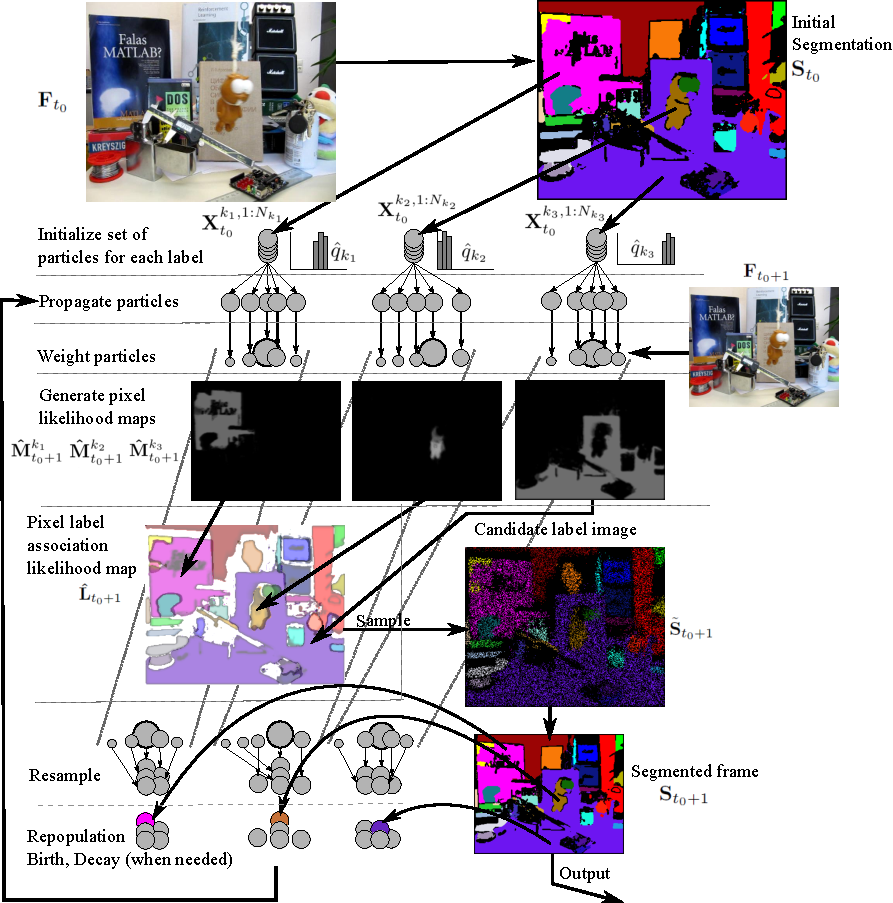
\includegraphics[width=\linewidth]{figures/ECCV2012/AlgorithmFlow2.pdf}
  \caption[Overview of Algorithm]{Flow of algorithm for one time step, shown for three labels ($k_1$, $k_2$, and $k_3$). For a description, see Section~\ref{sec:Overview}.}
\label{fig:AlgorithmFlow}
\end{figure}

The particles are then propagated in time independently, shifting their existence maps to new regions of the image. These shifted maps are used to generate measured color histograms from the next frame, which are evaluated to determine similarity to the object's reference histogram. The set of particles for each object is then combined to create an overall object pixel likelihood map. The pixel likelihood maps for all objects are then further combined with each other to create a label association likelihood map. In this likelihood map, each pixel is a \gls{pdf} specifying the probability that the original image pixel was generated from an observation of a particular object.

The label association likelihood map is then sampled using a per-pixel selection procedure (as described in Section~\ref{sec:LabelAssocLikelihoodMap}) to generate a candidate label image, $\tilde{\mathbf{S}}_{t_0+1}$. This candidate image is used as the initialization for the Metropolis-Hastings algorithm with annealing of Abramov et al. \cite{Abramov_RealtimeSegmentation}, which updates the labels iteratively until an equilibrium segmented state is reached. The segmentation result, $\mathbf{S}_{t_0+1}$  is subsequently used to update the set of particles via three mechanisms; birth, decay, and repopulation. Birth is used for new labels in the segmentation output, and consists of initializing a new set of particles. Decay occurs when a label is not found in the segmentation output, and consists of killing a number of the particles of the missing label. The most commonly occurring mechanism, repopulation, occurs for all previously existing object labels which are found. Repopulation rejuvenates the set of particles for an object by replacing a number of particles in the set with new particles based on the relaxed segmentation result. 

\section{Tracking Object Masks}
We shall now describe each of the parts of the algorithm given above in further detail, beginning with a description of how we track object masks using particle filters. First we will briefly review the basic principles of sequential Bayesian estimation and particle filtering, and then show how they can be used to predict pixel-level label associations in order to seed a segmentation algorithm.

\subsection{Sequential Bayesian Estimation}
Sequential Bayesian estimation uses a state space representation, in which a state vector $\mathbf{x}_t$ describes the hidden state of a dynamic system. Bayesian estimation attempts to determine the posterior distribution of the state given all prior observations $\mathbf{z}$, i.e., $\mathit{p}(\mathbf{x}_t|\mathbf{z}_{1:t})$. This is accomplished using a two step recursion which first generates a hypothesis of the current state conditioned on the previous state and then performs a Bayes update using the new observation. These steps are known as the prediction and filtering steps, respectively. 

The prediction step estimates the current distribution given all prior observations, or
\begin{equation} \label{eqn:prior}
\mathit{p}(\mathbf{x}_t|\mathbf{z}_{1:t-1}) =  \int{ \mathit{p}(\mathbf{x}_t|\mathbf{x}_{t-1})\mathit{p}(\mathbf{x}_{t-1}|\mathbf{z}_{1:t-1}) \mathit{d}\mathbf{x}_{t-1}}. 
\end{equation}
This prediction requires the specification of a stochastic \textit{dynamic model} 
\begin{equation} 
\mathbf{x}_t = \mathit{f}_t(\mathbf{x}_{t-1},\mathbf{v}_t) ,
\end{equation}
where $\mathbf{v}_t$ is the process noise, which characterizes the state transition density $\mathit{p}(\mathbf{x}_t|\mathbf{x}_{t-1})$. The dynamic model takes advantage of knowledge of the system to generate reliable predictions of how the state evolves. 

The filtering step uses Bayes rule to update the predicted density by conditioning it on the new observation $\mathbf{z}_t$:
\begin{equation} \label{eqn:posterior}
\mathit{p}(\mathbf{x}_t|\mathbf{z}_{1:t}) =  \frac{ \mathit{p}(\mathbf{z}_t|\mathbf{x}_{t})\mathit{p}(\mathbf{x}_{t}|\mathbf{z}_{1:t-1})} {\mathit{p}(\mathbf{z}_{t}|\mathbf{z}_{1:t-1})}. 
\end{equation}
This requires the specification of an observation, or measurement, model
\begin{equation} 
\mathbf{z}_t = \mathit{h}_t(\mathbf{x}_{t},\mathbf{w}_t) ,
\end{equation}
where $\mathbf{w}_t$ is the measurement noise, which characterizes the observation density $\mathit{p}(\mathbf{z}_t|\mathbf{x}_{t})$. Once the filtered, or posterior distribution is determined, an estimate of the state can be made using a variety of techniques (e.g., maximum a-posteriori, mean-shift). 

\subsubsection{Dynamic Model}
In our method, the state of a particle consists of four elements; the pixel existence map $\mathbf{M}$, a reference color histogram $\hat{q}$, a position shift vector $\mathbf{p}$, and a velocity vector $\mathbf{v}_t$. Of these, only the position shift and velocity evolve over time, so we adopt the state vector
 \begin{equation} 
 \mathbf{x}_t = [p_x v_x p_y v_y]^T ,
 \end{equation}
where $(p_x,p_y)$ denotes the accumulated shift of the pixel existence map in the image plane, and $(v_x,v_y)$ the map velocity in the image plane. Motion is modeled using a constant velocity model in discrete time with uniform sampling period $\mathit{T}$, giving the dynamic model
\begin{equation} \mathbf{x}_t = \mathbf{A}\mathbf{x}_{t-1} + \mathbf{v}_t , \end{equation}
where
\begin{equation} \mathbf{A} = 
\begin{bmatrix}
 1 & \mathit{T} & 0  & 0 \\ 
 0 & 1 & 0 & 0\\ 
 0 & 0 & 1 & \mathit{T}\\ 
 0 & 0 & 0 & 1
\end{bmatrix} \end{equation}
and noise $\mathbf{v}_t$ is assumed to be zero mean Gaussian with fixed covariance.

\subsubsection{Measurement Model}
In our method measurements are taken by calculating a color histogram, $\mathit{q}_t$ for the region lying within the shifted pixel existence map $\mathbf{M}$. That is, for particle $n$ of object $k$,
\begin{equation}
\mathit{q}^{k,n}_t = hist( \mathbf{F}_{t} \cap \mathbf{M}^{k,n}_t ).
\end{equation}
Color histograms are three dimensional, with 8 bins for each of the color components hue, saturation, and value. As in \cite{ColorBasedProbabilisticTracking}, a Gaussian density is used for the observation density $\mathit{p}(\mathbf{z}_t|\mathbf{x}_{t})$, that is
\begin{equation} 
\label{eqn:Weighting}
\mathit{p}(\mathbf{z}_t|\mathbf{x}_{t}) = \frac{1}{\sqrt{2\pi}\sigma} \exp{-\frac{\Delta(\hat{\mathit{q}},\mathit{q}_t)^2}{2\sigma^2}}, 
\end{equation}
where $\Delta(\mathit{\hat{q}},\mathit{q}_t)$ is the Bhattacharyya distance (as proposed in \cite{Real-timeTrackingMeanShift}) between the reference histogram $\mathit{\hat{q}}$ for the particle and the measured histogram $\mathit{q}_t$ for time $\mathit{t}$. The Bhattacharyya distance is a standard measure of similarity between discrete probability distributions, and is defined as
\begin{equation} \Delta(\hat{\mathit{q}},\mathit{q}_t) = \sqrt{1- \sum{\sqrt{\hat{\mathit{q}}\mathit{q}_t }}}. \end{equation}

\subsection{Parallel Particle Filters}
Except in special cases (e.g., Kalman Filter), closed-form solutions to Equations \eqref{eqn:prior} and \eqref{eqn:posterior} are not available. Particle Filters are a Monte-Carlo method designed to approximate the posterior distribution with a weighted set of random samples. There are many excellent descriptions of the mechanics of particle filtering available (such as \cite{Doucet2001}), so we shall avoid presenting them here, and proceed directly to presenting the details of our algorithm. 

The predictive portion of the method uses multiple Sequential Importance Resampling (SIR) filters in parallel to track multiple targets (labels) simultaneously. At this stage in the algorithm targets are assumed independent and interaction between labels is therefore not considered (interaction is accounted for later, as described in Section \ref{sec:Label Image Generation}). Particles are first propagated using the constant velocity dynamics model, and their predicted existence maps $\tilde{\mathbf{M}}^{k,n}$ are used to generate a measured histogram, $\mathit{q}_t$. Particles are weighted based on \eqref{eqn:Weighting}, and then normalized as a set for each label $k$. Systematic resampling is used to prevent particle degeneracy, due to its speed and good empirical performance \cite{Doucet2001}.

The resulting distributions from the weighting procedure are used to generate object pixel likelihood maps for each label,$\hat{\mathbf{M}}^{k}_{t+1}$, which are then combined into the label association likelihood map $\hat{\mathbf{L}}_t$, as described in Section \ref{sec:Label Image Generation}. A realization of this likelihood map can then be relaxed to produce a final segmented output, $\mathbf{S}_t$. 

\subsection{Particle Birth, Repopulation, \& Decay.}
One key improvement of the proposed algorithm over prior particle filtering methods is its use of the segmentation result $\mathbf{S}_{t}$ to update the particle sets. This allows the creation of new targets, adaptation to changing target appearance, and gradual elimination of targets which are no longer observed. This is accomplished via three mechanisms, which we term, respectively, birth, repopulation, and decay. 

Birth occurs when a label which has not existed previously is found in the segmentation output $\mathbf{S}_{t}$, or more formally $ \{ k\notin \mathbf{S}_{1:t-1}, k\in \mathbf{S}_{t}\}$. It consists of generating a set of particles $\mathbf{X}^k$ for the new label using $\mathbf{S}_{t}$ to initialize an existence map $\mathbf{M}^k_t$ and $\{\mathbf{F}_{t} \cap \mathbf{M}^k_t \}$ to calculate a reference color histogram $\hat{\mathit{q}^k_t}$.

Repopulation is a key component of the algorithm, as it allows the pixel likelihood map for an object, $\mathbf{\hat{M}}^k$, to adapt over time to the changing appearance of the object. Every iteration, all previously existing object labels which are found in $\mathbf{S}_{t}$ are repopulated by replacing some particles in the set with particles generated from $\mathbf{S}_{t}$ and $\mathbf{F}_{t}$. Particles are chosen for replacement using stratified sampling, at a rate specified by parameter $\lambda_r$. The repopulation mechanism gradually modifies the object "model" through the addition of particles which have an updated existence map and color histogram (coming from the segmentation result). We use the term model here loosely, since there is in actuality no explicit model for any of the objects - merely a pixel likelihood map generated at each time step from the objects constituent particles and the current image frame. 

Stratified replacement and relatively low repopulation rates are used to help keep the influence of erroneous hypotheses to a minimum, but as with any adaptive method, they can occasionally lead the tracker astray. Replacement of particles, rather than updating of a central model, helps to reduce this problem, since a few erroneous particles will generally not completely derail the algorithm. Nevertheless, future work could investigate strategies that allow pruning of unlikely hypotheses without negatively affecting occlusion handling. 

Decay occurs when a label is not found in the segmentation output, $ k \notin \mathbf{S}_t $. Particles are selected from $k$ using random sampling, at a rate determined by the decay rate $\lambda_d$, and are pruned; they are no longer considered when filtering $k$. This reduces the number of active particles for the label in the next iteration, $N^k_{t+1}$, by approximately $\lambda_d N^k_t$. If the number of active particles for a label falls below a certain threshold, $N_{min}$, then the set of particles for the label is deleted, and the object is no longer tracked. If a label which was being decayed is observed again, i.e., $ \{ k\notin \mathbf{S}_{t-1}, k\in \mathbf{S}_{t}\}$, then the label is revived by replacing particles which had been killed with new particles, which are initialized as in the repopulation step.

\section{Extracting a Dense Image Labeling}
\label{sec:Label Image Generation}

The middle portion of Figure \ref{fig:AlgorithmFlow} depicts how the candidate label image,  $\tilde{\mathbf{S}}_{t}$, is generated. The candidate label image is a summary of the accumulated knowledge of the particle filters; it is a prediction of what the segmented scene should look like. That is to say, it is a pixel-wise realization of the label association likelihood map $\hat{\mathbf{L}}_{t}$, which is constructed by combining the object pixel likelihood maps (which approximate the posteriors of the particle sets). $\tilde{\mathbf{S}}_{t}$ is the seed of the segmentation kernel, which uses pixel values from $\mathbf{F}_t$  to perform the relaxation process and generate a dense label image. In this section we will describe the process of generating the object pixel and label association likelihood maps, and then explain how the predictive loop allows occlusion handling without explicit object relationships or depth modeling.

\subsection{Object Pixel Likelihood Maps.}
The object pixel likelihood map for a particular object $k$ is the weighted sum of the pixel existence maps of all of its labels,
\begin{equation}
\label{eqn:PixelLikelihood}
\hat{\mathbf{M}}^{k}_{t} = \sum_{n=1}^{N_k}w^{k,n}_t \mathbf{M}^{k,n} .
\end{equation}
Because the weights have been normalized, the pixel values in $\hat{\mathbf{M}}^{k}_{t}$ will be in the range $[0,1]$. High pixel values will occur in regions which are present in the existence maps of highly weighted particles, or alternatively, are present in many particles with average weight. 

\subsection{Label Association Likelihood Map.}
\label{sec:LabelAssocLikelihoodMap}
The label association likelihood map $\hat{\mathbf{L}}_{t}$ is a combination of all the object pixel likelihood maps, such that each pixel contains a discrete probability distribution giving the likelihood of the pixel belonging to a certain label.  Additionally, a likelihood, $p_0$, for the pixel belonging to no label is inserted to allow pixels where no label has high likelihood to remain unlabeled in  $\tilde{\mathbf{S}}_{t}$. More formally, 
\begin{equation}
\hat{\mathbf{L}}_{t} = \bigcup_{n=1}^{K} \hat{\mathbf{M}}^{n}_{t} + p_0. 
\label{eqn:LabelMap}
\end{equation}
Each pixel of $\hat{\mathbf{L}}_{t}$ is then normalized, such that the sum of the discrete probabilities sums to one. The candidate label image can then be generated by taking a realization of $\mathbf{\hat{L}}_{t}$ to select pixel label values. Examples of the result of this process, $\tilde{\mathbf{S}}_{t}$, can be seen in Figures \ref{fig:AlgorithmFlow} and \ref{fig:Results}.

\section{Occlusion Handling.}
Occlusion relationships are handled naturally, since foreground objects will tend to have a strong peak in their weight distribution, corresponding to those particles which align properly with $\mathbf{F}_t$. Objects they occlude will have a flat particle weight distribution, since there will exist no shifted existence map which contains a color distribution which matches the reference histogram. This is due to the fact that the occluding objects and objects surrounding the occluded object have color distributions which differ from the occluded object. Let us assume foreground object j is contained by occluded object k, that is
\begin{equation}
\label{eqn:subset}
\mathbf{M}^{j,n}_t \subset \mathbf{M}^{k,n}_t .
\end{equation}
We also assume that the number of particles is sufficiently large such that
\begin{equation}
\label{eqn:truth}
\exists~\mathbf{M}^{j,n}_t \in \mathbf{M}^{j}_t : hist(\mathbf{F}_{t} \cap \mathbf{M}^{j,n}_t) \approx \hat{q}^{j,n}.
\end{equation}
If $hist(\mathbf{F}_{t} \cap \mathbf{M}^{k,n}) \neq hist(\mathbf{F}_{t} \cap \mathbf{M}^{j,n})$, that is, the objects have different color distributions, then from \eqref{eqn:subset} and \eqref{eqn:truth}, it follows that \footnote{This also assumes that the areas surrounding the occluded object also have different color distributions.}
\begin{equation}
\label{eqn:notruth}
\nexists~\mathbf{M}^{k,n}_t \in \mathbf{M}^{k}_t : hist(\mathbf{F}_{t} \cap \mathbf{M}^{k,n}_t) \approx \hat{q}^{k,n}
\end{equation}
and therefore that 
\begin{eqnarray}
min_{1:N_j} \{ \Delta(\hat{\mathit{q}^{j,n}},hist(\mathbf{F}_{t} \cap \mathbf{M}^{j,n}_t) )\} < \nonumber \\
min_{1:N_k} \{ \Delta(\hat{\mathit{q}^{k,n}},hist(\mathbf{F}_{t} \cap \mathbf{M}^{k,n}_t) )\}
\end{eqnarray}
and thus
\begin{equation}
max_{1:N_j}\{w^{j,n}_t\} > max_{1:N_k}\{w^{k,n}_t\}.
\end{equation}
This means that in the label association likelihood map $\hat{\mathbf{L}}_{t}$, the occluding object will have a higher likelihood then the occluded. The candidate label image, $\tilde{\mathbf{S}}_{t}$ will therefore tend to favor occluding object labels, which will dominate the occluded object label during the segmentation relaxation process.

\section{Segmentation using Superparamagnetic Clustering}
To adjust the candidate label image $\tilde{\mathbf{S}}_{t}$ to the current frame $\mathbf{F}_{t}$, we use a real-time image segmentation algorithm based on superparamagnetic clustering of data \cite{Blatt_SuperClustering}. The method of superparamagnetic clustering represents an input image being segmented by a Potts model, with pixel color vectors arranged on the sites of a two-dimensional (2D) lattice, where each pixel is featured by an additional variable, called a spin. This allows the segmentation problem to be formulated as a minimization problem which seeks to find the equilibrium states of the energy function in the superparamagnetic phase. In this equilibrium state regions of aligned spins coexist and correspond to a natural partition of the image data \cite{Blatt_SuperClustering}. Since every found segment carries a spin variable which is unique within the whole image, the terms {\em spin} and {\em label} are equivalent here. The equilibrium states are found by the use of the highly parallel 
Metropolis algorithm with a simulated annealing, called {\em relaxation process}, implemented on a Graphics Processing Unit (GPU) \cite{Abramov_RealtimeSegmentation}. In this work, the relaxation process adjusts the predicted candidate label image to the current frame. 

\begin{figure}
\label{fig:Convergence}
\centering
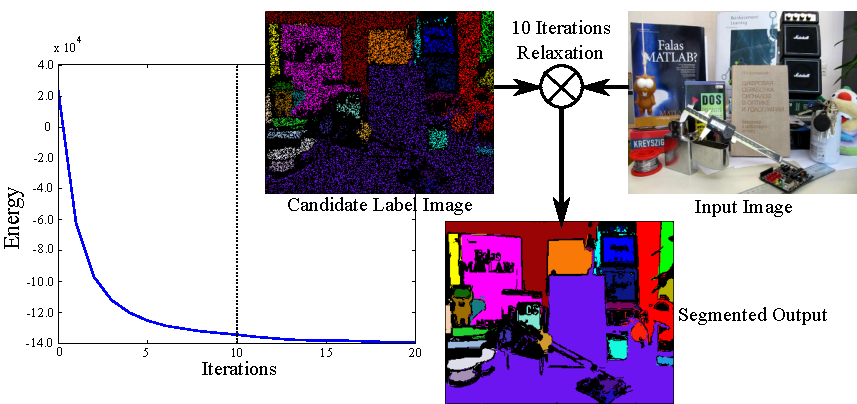
\includegraphics[width=\linewidth]{figures/ECCV2012/ConvergenceFig2.pdf}
\caption[Relaxation Convergence]{The relaxation process causes the energy of the label image to converge after few iterations (outcome after 10 iterations shown here). This results in efficient calculation of an accurate and temporally coherent segmentation.}
\label{fig:Convergence}
\end{figure}

Superparamagnetic clustering of data was chosen due to its flexibility in allowing the use of any initialization state; there are no particular requirements to the initial states of spin variables. The closer the initial states are to the equilibrium, the less time the Metropolis algorithm needs to converge. This property makes it possible to achieve temporal coherency in the segmentation of temporally adjacent frames by using the sparse label configuration taken from the candidate label image for the spin initialization of the current frame. A final (dense) segmentation result is obtained within a small number of Metropolis updates. Conventional segmentation methods do not generally have this property and cannot turn a sparse segmentation prediction into dense final segments which preserve temporal coherence. Moreover, since the method can directly use sparse predictions as the seed of the segmentation kernel, we can avoid the costly and error-prone block-matching procedure required to find label correspondences in other 
work, such as in Brendel and Todorovic \cite{SegTrackRegions} or Hedau et al.  \cite{MatchingUnstable}. Figure \ref{fig:Convergence} illustrates the relaxation process, and the convergence of energy after a small number of iterations. 

\section{Experimental Results}
\label{sec:Experimental Results}

In order to evaluate performance, we compare our method to the state of the art on several challenging video tracking benchmark sequences which are available online\footnote{http://www.GPU4Vision.org}. It should be noted that, as opposed to the other tracking algorithms, we do not pre-select a region to track, and track fully deforming object masks (rather than a rectangle). Additionally, we employ no learned or a-priori specified models, use 50 particles per label, and only have two parameters; the repopulation and decay rates $\lambda_r$ and $\lambda_d$, which were both held constant at $0.05$ throughout testing. Results are compared to the PROST \cite{PROST}, MilTrack \cite{MilTrack}, FragTrack \cite{FragTrack}, and ORF \cite{ORF} tracking algorithms. Further details concerning the parameters used for the above algorithms in the benchmarking can be found in \cite{PROST}.

We shall not evaluate the visual quality of segmentation results here for a couple of reasons. First, detailed evaluation of the visual quality of super-paramagnetic clustering has been presented in \cite{Abramov_RealtimeSegmentation} in great detail. The visual quality of the segmentation results obtained from this work do not differ significantly from these results, with the exception of labels having continuity through occlusions. Secondly, it is directly acknowledged in other \gls{vos} work that the methods fail under partial \cite{MSVS,PropValAgg} or full \cite{SegTrackRegions,MHVS} occlusions. As such, comparing performance to other \gls{vos} methods is somewhat unreasonable. Rather, the better comparison is to the state of the art in tracking methods, which attempt to handle full and partial occlusions.

In order to compare with the other methods, we needed to output a tracking rectangle for each frame. To do this, once the sequence was segmented, we found the segment which corresponded to the object to track in the first frame, and then took the bounding-box which contained it in each frame as the tracking rectangle. This bounding-box was then compared to ground-truth using two measures; Euclidean distance and the PASCAL-challenge based score proposed in \cite{PROST}. The latter compares the area of intersection of the ground truth and tracked box with the union of the same. When this is greater than 0.5, the object is considered successfully tracked. Table \ref{table:results} gives our results, as well as the results for the other methods.
 
 \begin{table}
\caption{PROST dataset benchmark results. Top and bottom tables are average pixel error and PASCAL based scores, respectively}
\begin{center}
\begin{tabular}{|l|c|c|c|c|c|c|}
\hline
Sequence &  PROST  & MIL & Frag & ORF & HybridPF \\
\hline\hline
Lemming & 25.1 & 14.9 & 82.8 & 166.3 & 19.8\\
Box & 13.0 & 104.6 & 57.4 & 145.4 & 114.1\\
Liquor & 21.5 & 165.1 & 30.7 & 67.3 & 25.5\\
Board & 39.0 & 51.2 & 90.1 & 154.5 & 30.9\\
\hline
\hline
\hline\hline
Lemming & 70.5 & 83.6 & 54.9 & 17.2 & 73.9\\
Box & 90.6 & 24.5 & 61.4 & 28.3 & 7.5\\
Liquor & 85.4 & 20.6 & 79.9 & 53.6 & 54.2\\
Board & 75.0 & 67.9 & 67.9 & 10.0 & 71.4\\
\hline
\end{tabular}
\end{center}

\label{table:results}
\end{table}


Testing showed that, when certain assumptions hold, our algorithm performs on par with, and in some cases outperforms, state of the art tracking algorithms. This is the case for the \textit{liquor}, \textit{lemming}, and \textit{board} sequences. In the \textit{lemming} sequence, frames of which are shown in Figure \ref{fig:Results}, our algorithm outperforms the other methods in cases of occlusion, especially when the tracked object is fully occluded. While other methods offer false positives and erroneous tracks, our method decays the label for the object and avoids proposing incorrect tracking solutions. In the \textit{liquor} sequence, our algorithm adapts to the changing appearance (size, shape, and color) of the tracked bottle, allowing it to maintain performance on par with the other algorithms, in spite of the difficulties of segmenting transparent objects. In the \textit{board} sequence, our method successfully adapts to the rapidly changing appearance of the tracked board as it rotates, allowing it to maintain an accurate track and outperform the other methods.

In addition to showing the strengths of our method, a weakness was also highlighted by the benchmark sequences. The \textit{box} sequence demonstrated the limitations of using unsupervised color-based segmentation to initialize the objects to track. In the sequence, the object to track contains strong color differences, which are segmented into different initial regions. As the object moves around, the particles for these regions are attracted to other objects it passes over which have similar color.  

%color histograms as a measurement. In the sequence, the black box being tracked passes in front of another black box several times. In almost all cases, particles are attracted to the other box, which results in twin peaks in $\mathbf{\hat{M}}^k_{t}$. While the tracked object is not lost, this results in the final segmented output having the same label for both boxes.

\begin{figure}[t]
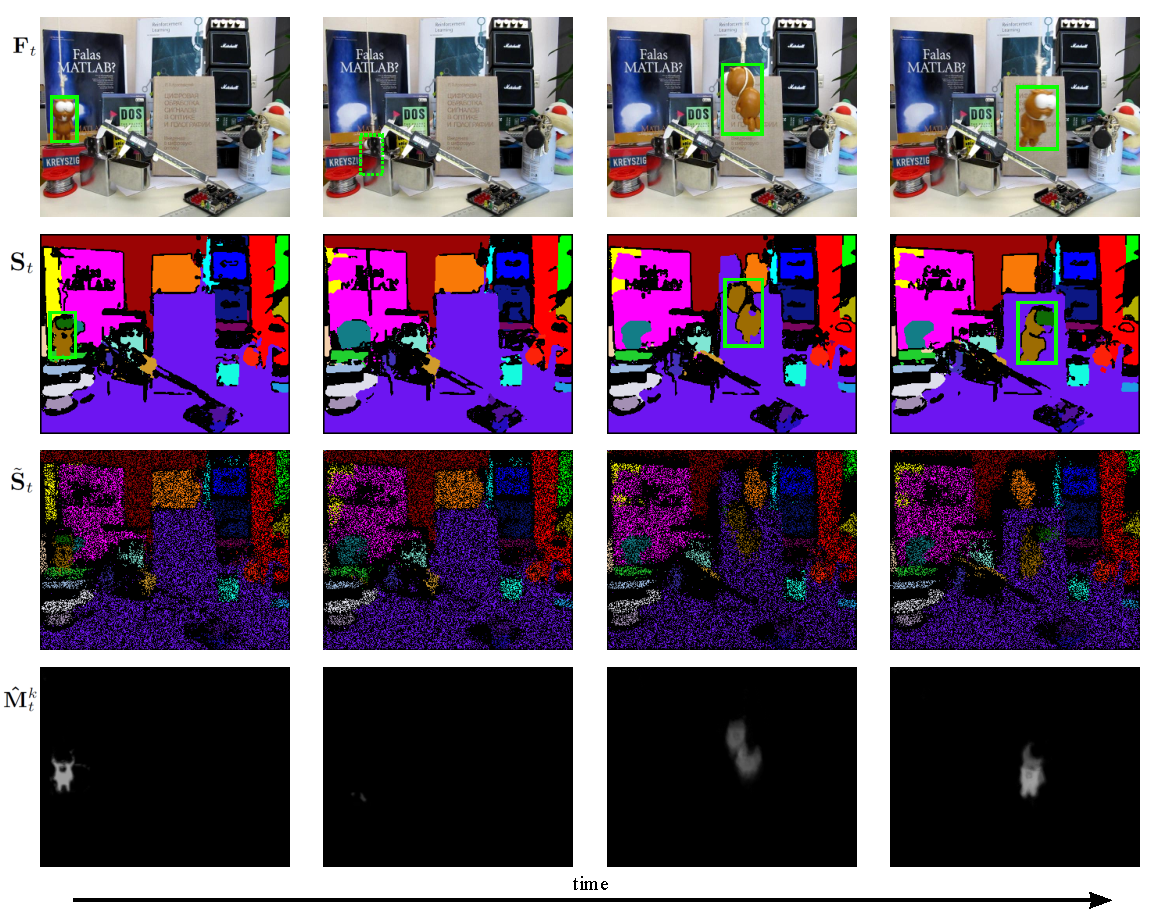
\includegraphics[width=\linewidth]{figures/ECCV2012/Tracking.pdf}
  \caption[Tracked output from lemming sequence]{Output frames from the \textit{lemming} sequence, in which a target is completely occluded (for $\sim20$ frames, second column) and changes significantly in appearance. The object which is tracked for comparison to other algorithms is highlighted with a green box. $\mathbf{F}_t$-Original frames from  movie.~~$\mathbf{S}_t$-The output of the segmentation algorithm.~~$\tilde{\mathbf{S}}_{t}$-The candidate label image constructed by taking a random draw from $\hat{\mathbf{L}}_{t}$, the label association likelihood map.~~$\hat{\mathbf{M}}^k_{t}$-The overall object pixel likelihood map for the lemming label, created by combining the set of particles for the label. Intensity represents the sum of the normalized weights of the set of particles.}
\label{fig:Results}
\end{figure}

\begin{figure}[t]
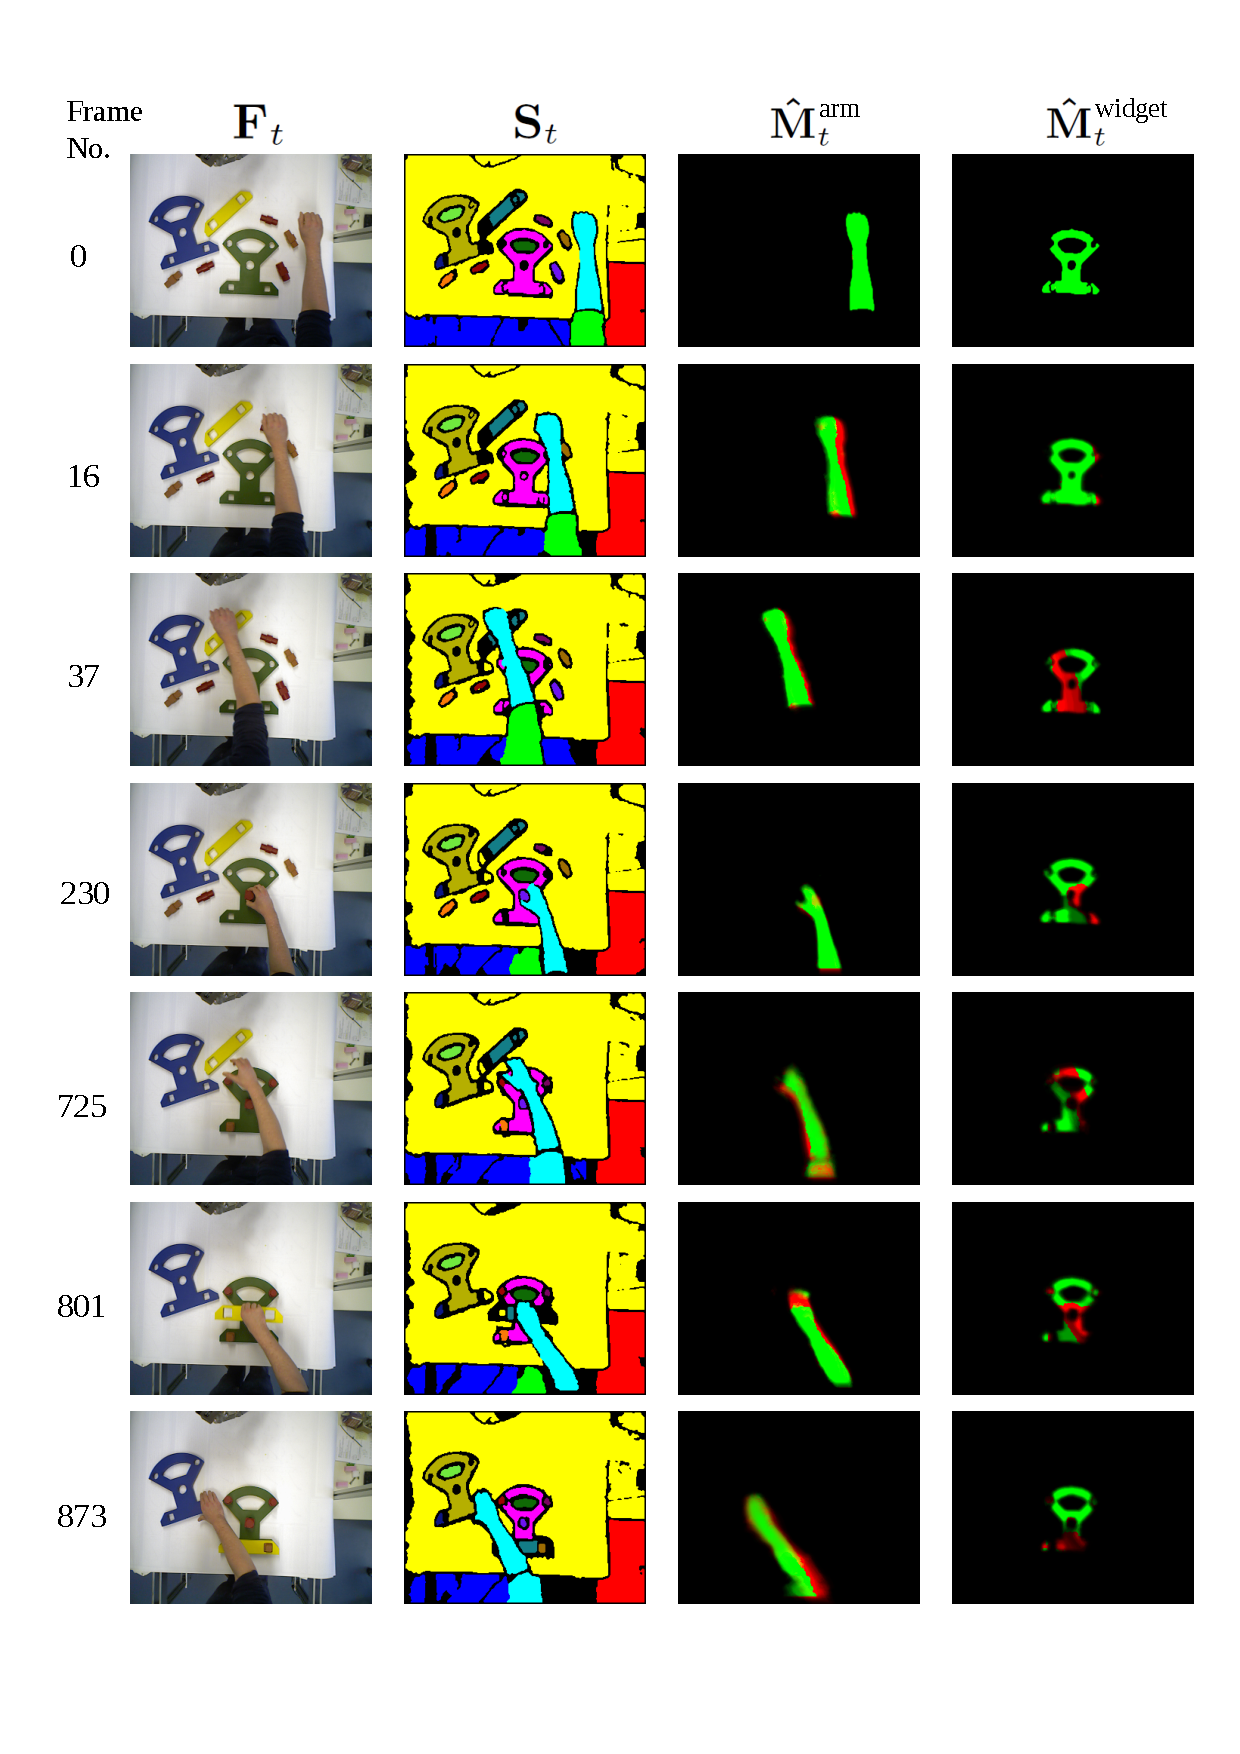
\includegraphics[width=\linewidth]{figures/ECCV2012/Cranfield_Results.pdf}
  \caption[Results of Cranfield Sequence]{Results of segmentation on Cranfield Benchmark Sequence. Green masks show observed pixels, while red masks show occluded pixels which are believed to belong to the object.}
\label{fig:Cranfield_Results}
\end{figure}

\section{Discussion}
In this chapter we presented a new method for performing on-line, dense, unsupervised video segmentation which uses tracking as the basis for segmentation. We have given results which show that the method is able to resolve occlusion relations between objects without explicitly modeling them, and can maintain consistent labels for objects, even when they leave and re-enter the field of view. Additionally, we have shown that the method is able to adapt to rapidly changing appearance of tracked objects, producing consistent segmentations over lengthy video sequences. A GPU version of the algorithm has been developed that can achieve near real-time levels ~10 fps at 640x480 resolution on an i7 standard desktop. One sequence we tested showed the vulnerability of the method to situations where objects have similar color distributions. A way to resolve this is to consider additional features such as object geometry in the measurement function. To measure such geometric features requires the addition of depth to our observations; we shall investigate adding this extra dimension in the following chapters. 



\begin{savequote}[75mm]
The world is a construct of our sensations, perceptions, memories. It is convenient to regard it as existing objectively on its own. But it certainly does not become manifest by its mere existence.
\qauthor{Erwin Sch\"{o}dinger}
\end{savequote}
%For an example of a full page figure, see Fig.~\ref{fig:myFullPageFigure}.

\chapter{Patch-based Perceptual World Model}
\label{Chap:WorldModel}
\lettrine[lines=3, loversize=0.3]{\textcolor{DarkBlue}T}{he widespread availability of cheap 3D sensors} has had a profound impact on the world of computer vision. Researchers have found that they no longer need to attempt to find heuristic tricks which can create an artificial three dimensional interpretation from a two dimensional image. The advent of the Kinect (and other, related inexpensive RGB-D sensors) has allowed direct progression to high-level concepts and rules which the human mind uses when first learning to understand the real world - a completely different approach than trying to mimic the behavior of the mind when it is adapting those rules (learned from a life-time of 3D stereo data) in order to interpret some new 2D image.

In this chapter we shall present our work in creating a full 3D artificial world model which can be used for higher level semantic understanding of both single frames and video. The model we present begins with point clouds, relying on the general framework set up in the Point Cloud Library \footnote{\url{http://www.pointclouds.org/}} (which we have both made use-of and contributed-to extensively as part of this work). Point clouds are a useful way of representing the data obtained from RGB-D sensors. The pixel coordinates and depth value coming from the RGB-D pair can be transformed into an $(x,y,z)$ point, and the RGB information can be attached to this point.

\section{Pre-processing of Point Cloud Data}
Before continuing, we shall briefly introduce two pre-processing steps which are used throughout the rest of this work. The first downsamples the continuous point cloud space onto a discrete grid, while the second pre-computes an adjacency graph for this grid.

\subsection{Voxelization}
The resolution of a standard RGB-D camera such as the Kinect is 640x480 pixels, yielding about 300,000 points per frame. While for static image segmentation this might be an acceptable amount of data, for video segmentation it is simply too much data to process directly in reasonable run times (on standard hardware). Because of this, a common pre-processing step is to down-sample point clouds using a \textit{voxel-grid} filter, a process known as \textit{voxelization}. 

\begin{figure}
\begin{center}
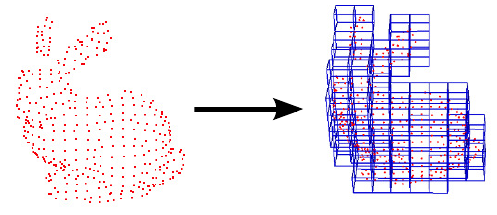
\includegraphics[width=0.8\linewidth]{figures/WorldModel/stanford_bunny.png}
\end{center}
   \caption[Example of Voxelization]{Illustration of Voxelization. On the left we have a point cloud of the ``Stanford Bunny''. This cloud is inserted into the voxel grid shown on the right, where all points falling within on grid unit, or voxel, are combined. From \cite{PCLWebsite}}
\label{fig:stanford_bunny}
\end{figure}
%------------------------------------------------------------------------

\begin{figure}
\begin{center}
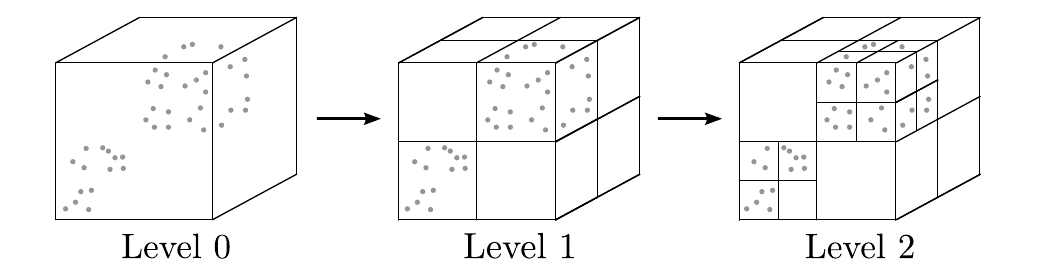
\includegraphics[width=\linewidth]{figures/WorldModel/voxel_grid_octree.png}
\end{center}
   \caption[Octree Voxelization]{Use of an octree for voxelization. The points are grouped into voxels by recursively subdividing the bounding box into its eight constituent octants. This recursion terminates when the box size has edge length equal to the voxel leaf size ${R}_{voxel}$.}
\label{fig:stanford_bunny}
\end{figure}

\begin{figure}
\begin{center}
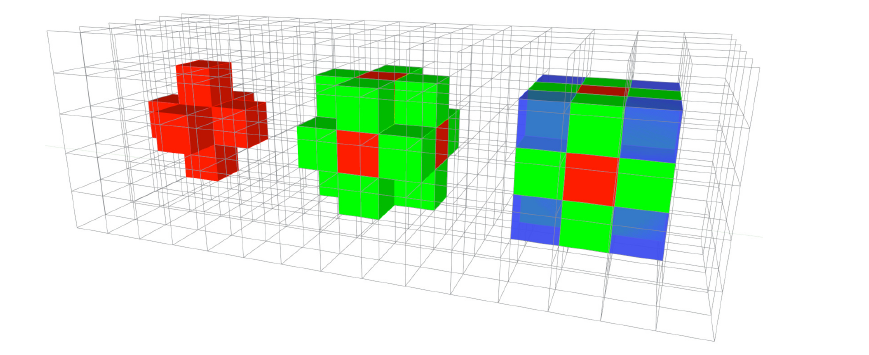
\includegraphics[width=0.9\linewidth]{figures/WorldModel/3d_nearest_neigh.png}
\end{center}
   \caption[Adjacency in a 3d Grid]{Adjacency in a 3d voxel grid. The 6-, 18-, and 26-neighborhoods share a face, edge, and vertex, respectively.}
\label{fig:3d_adjacency}
\end{figure}

\subsection{Octree Adjacency Graph}
\label{subsec:Adjacency}
In order to increase computational efficiency, we have developed an adjacency octree which maintains neighbor information within the octree leaves (i.e., the voxels). Adjacency is a key element of many methods, especially region growing algorithms, as it ensures that labels do not cross object boundaries which are disconnected in space. There are three definitions of adjacency in a voxelized 3D space; 6-,18-, or 26-adjacent. These share a face, faces or edges, and faces, edges, or vertices, respectively. In this work we use 26-adjacency exclusively, as the other lesser adjacencies might miss connections when surfaces are placed in certain configurations relative to the camera plane.

Throughout the rest of this work, we shall deal exclusively with voxels, rather than points, and shall always use our adjacency octree. As voxelization is a necessary pre-processing step for all of the algorithms we shall subsequently discuss, it can be assumed that adjacency information is always available in constant time. This is especially important for the clustering algorithm we introduce next.

\section{Geometrically Constrained Supervoxels}
\label{sec:Supervoxels}
In this Section we present  \acrfull{vccs}, a new method for generating superpixels and supervoxels from 3D point cloud data. The supervoxels produced by \gls{vccs} adhere to object boundaries better than state-of-the-art methods while remaining efficient enough to use in online applications. VCCS uses a variant of k-means clustering for generating its labeling of points, with two important constraints:

1. The seeding of supervoxel clusters is done by partitioning 3D space, rather than the projected image plane. This ensures that supervoxels are evenly distributed according to the geometry of the scene.

2. The iterative clustering algorithm enforces strict spatial connectivity of occupied voxels when considering points for clusters. This means that supervoxels strictly cannot flow across boundaries which are disjoint in 3D space, even though they are connected in the projected plane.
 
First, in \ref{subsec:Seeding} we shall describe how supervoxel seeds are generated and filtered, in \ref{subsec:Features} the features and distance measure used for clustering, and finally in \ref{subsec:FlowClustering} how the iterative clustering algorithm enforces spatial connectivity. Unless otherwise noted, all processing is being performed in the 3D voxelized space constructed from one or more RGB+D cameras (or any other source of point-cloud data). Furthermore, because we work exclusively in a voxel-cloud space (rather than the continuous point-cloud space), we shall adopt the following notation to refer to voxel at index $i$ within voxel-cloud $V$ of voxel resolution $r$:
\begin{equation} \label{eqn:Voxel}
{V}_{r}(i) = \mathbf{F}_{1..n}, 
\end{equation}
where $\mathbf{F}$ specifies a feature vector which contains $n$ point features (e.g. color, location, normals). 

\subsection{Spatial Cluster Seeding}
\label{subsec:Seeding}
The algorithm begins by selecting a number of seed points which will be used to initialize the supervoxels. In order to do this, we first divide the space into a voxelized grid with a chosen resolution ${R}_{seed}$, which is significantly higher than ${R}_{voxel}$. The effect of increasing the seed resolution ${R}_{seed}$ can be seen in Figure~\ref{fig:SegmentedDiffSeeds}. Initial candidates for seeding are chosen by selecting the voxel in the cloud nearest to the center of each occupied seeding voxel.    

Once we have candidates for seeding, we must filter out seeds caused by noise in the depth image. This means that we must remove seeds which are points isolated in space (which are likely due to noise), while leaving those which exist on surfaces. To do this, we establish a small search radius ${R}_{search}$ around each seed, and delete seeds which do not have at least as many voxels as would be occupied by a planar surface intersecting with half of the search volume (this is shown by the green plane in Figure~\ref{fig:SeedingDiagram}). Once filtered, we shift the remaining seeds to the connected voxel within the search volume which has the smallest gradient in the search volume. Gradient is computed as
\begin{equation} \label{eqn:Gradient}
\mathit{G}(i) = \sum_{k\in{V}_{adj}}{\frac{\parallel{V(i)-V(k)}\parallel{}_{CIELab}}{{N}_{adj}}};
\end{equation}
we use sum of distances in CIELAB space from neighboring voxels, requiring us to normalize the gradient measure by number of connected adjacent voxels ${N}_{adj}$. Figure~\ref{fig:SeedingDiagram} gives an overview of the different distances and parameters involved in seeding.

%------------------------------------------------------------------------
\begin{figure}
\begin{center}
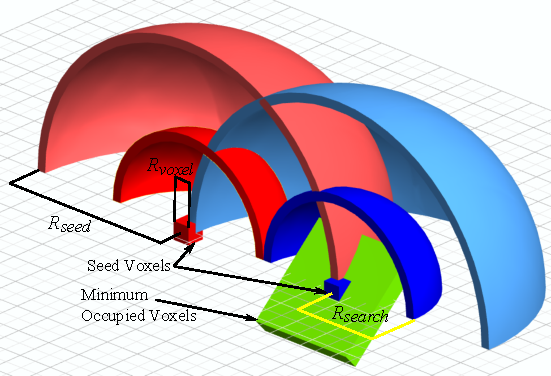
\includegraphics[width=0.9\linewidth]{figures/CVPR2013/MinimumOccupied.pdf}
\end{center}
   \caption[Seeding Parameters]{Seeding parameters and filtering criteria. ${R}_{seed}$ determines the distance between supervoxels, while ${R}_{voxel}$ determines the resolution to which the cloud is quantized. ${R}_{search}$ is used to determine if there are a sufficient number of occupied voxels to necessitate a seed. }
\label{fig:SeedingDiagram}
\end{figure}
%------------------------------------------------------------------------
%------------------------------------------------------------------------
\begin{figure}
\begin{center}
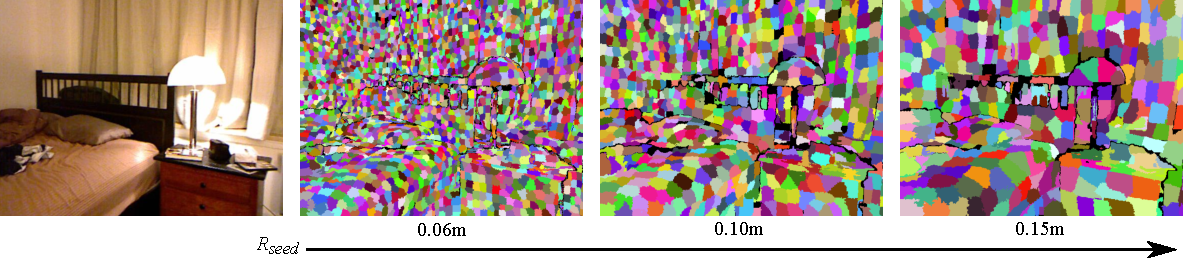
\includegraphics[width=1.0\linewidth]{figures/CVPR2013/IncreasingSeedSize.pdf}
\end{center}
   \caption[Seeding Size]{Image segmented using \gls{vccs} with seed resolutions of 0.1, 0.15 and 0.2 meters.}
\label{fig:SegmentedDiffSeeds}
\end{figure}
%------------------------------------------------------------------------
Once the seed voxels have been selected, we initialize the supervoxel feature vector by finding the center (in feature space) of the seed voxel and connected neighbors within 2 voxels. 

\subsection{Cluster Features and Distance}
\label{subsec:Features}
\gls{vccs} supervoxels are clusters in a 39 dimensional space, given as 
\begin{equation}
\label{eqn:FeatureSpace}
\mathbf{F} = [x,y,z,L,a,b,\textrm{FPFH}_{1..33}],
\end{equation}
where $x,y,z$ are spatial coordinates, $L,a,b$ are color in CIELab space, and $\textrm{FPFH}_{1..33}$ are the 33 elements of Fast Point Feature Histograms (FPFH), a local geometrical feature proposed by Rusu et al.\@ \cite{FPFH}. FPFH are pose-invariant features which describe the local surface model properties of points using combinations of their \textit{k} nearest neighbors. They are an extension of the older Point Feature Histograms optimized for speed, and have a computational complexity of $O(n \cdot k)$.  

In order to calculate distances in this space, we must first normalize the spatial component, as distances, and thus their relative importance, will vary depending on the seed resolution ${R}_{seed}$. Similar to the work of Achanta et al.\@, \cite{SLICCompared} we have limited the search space for each cluster so that it ends at the neighboring cluster centers. This means that we can normalize our spatial distance $D_s$ using the maximally distant point considered for clustering, which will lie at a distance of $\sqrt{3} {R}_{seed}$. Color distance $D_c$, is the euclidean distance in CIELab space, normalized by a constant $m$. Distance in FPFH space, $D_f$, is calculated using the Histogram Intersection Kernel \cite{HistogramIntersection}. This leads us to a equation for normalized distance $D$:
\begin{equation}
\label{eqn:Distance}
D = \sqrt{\frac{\lambda D_c^2}{m^2}+\frac{\mu D_s^2}{3 {R}_{seed}^{2}}+\epsilon {D}_{HiK}^{2}},
\end{equation}
where $\lambda,\mu,$ and $\epsilon$ control the influence of color, spatial distance, and geometric similarity, respectively, in the clustering. In practice we keep the spatial distance constant relative to the other two so that supervoxels occupy a relatively spherical space, but this is not strictly necessary. For the experiments in this paper we have color weighted equally with geometric similarity.

\subsection{Flow Constrained Region Growing}
\label{subsec:FlowClustering}
Assigning voxels to supervoxels is done iteratively, using a local k-means clustering related to \cite{SLICCompared,DASP}, with the significant difference that we consider connectivity and flow when assigning pixels to a cluster. The general process is as follows: beginning at the voxel nearest the cluster center, we flow outward to adjacent voxels and compute the distance from each of these to the supervoxel center using Equation \ref{eqn:Distance}. If the distance is the smallest this voxel has seen, its label is set, and using the adjacency graph, we add its neighbors which are further from the center to our search queue for this label. We then proceed to the next supervoxel, so that each level outwards from the center is considered at the same time for all supervoxels. We proceed iteratively outwards until we have reached the edge of the search volume for each supervoxel (or have no more neighbors to check).

%------------------------------------------------------------------------
\begin{figure}
\begin{center}
   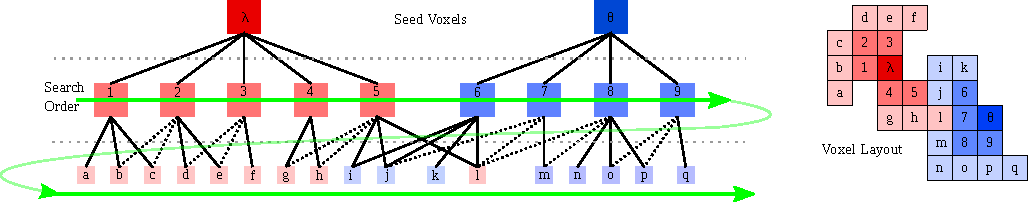
\includegraphics[width=0.95\linewidth]{figures/CVPR2013/SearchOrder.pdf}
\end{center}
   \caption[Voxel Search Order]{Search order for the flow constrained clustering algorithm (shown in 2D for clarity). Dotted edges in the adjacency graph are not searched, as the nodes have already been added to the search queue.}
\label{fig:ClusterSearch}
\end{figure}
%------------------------------------------------------------------------

This amounts to a breadth-first search of the adjacency graph, where we check the same level for all supervoxels before we proceed down the graphs in depth. Importantly, we avoid edges to adjacent voxels which we have already checked this iteration. The search concludes for a supervoxel when we have reached all the leaf nodes of its adjacency graph or none of the nodes searched in the current level were set to its label. This search procedure, illustrated in Figure~\ref{fig:ClusterSearch}, has two important advantages over existing methods:

1. Supervoxel labels cannot cross over object boundaries that are not actually touching in 3D space, since we only consider adjacent voxels, and 

2. Supervoxel labels will tend to be continuous in 3D space, since labels flow outward from the center of each supervoxel, expanding in space at the same rate.

Once the search of all supervoxel adjacency graphs has concluded, we update the centers of each supervoxel cluster by taking the mean of all its constituents. This is done iteratively; either until the cluster centers stabilize, or for a fixed number of iterations. For this work we found that the supervoxels were stable within a few iterations, and so have simply used five iterations for all presented results. 

\section{Sequential Update of Perceptual Model}
As an additional consideration, we have developed a scheme for adding new point clouds sequentially (as from a video stream) into an existing supervoxel octree. This is accomplished through a process which classifies voxels in the tree based on their behavior. As a first step, we insert points from the new point cloud into the octree, and initialize new leaves for voxels which did not exist previously. This results in an octree where leaves fall into three possible categories (illustrated in Fig.~\ref{fig:VoxelVisibility}; they are either new, observed, or unobserved in the most recent observation. Handling of new leaves is straightforward; we simply calculate adjacency relations to existing leaves and flag them as unlabeled. 
\begin{figure}
  \centering
  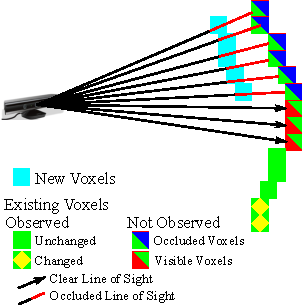
\includegraphics[scale=1.5]{figures/IROS2013/VoxelVisibility.pdf}
  \caption[Voxel Visibility]{Categorization of voxels based on new frame of data. Voxels fall into three categories, they are either new, observed or not observed in the frame. Furthermore, observed voxels can either have changed or remained the same, while voxels not observed in the frame are either occluded or no longer exist (in which case they should be deleted).}
  \label{fig:VoxelVisibility}
\end{figure}

To determine whether a leaf which existed previously has changed, we test the distance between the centroid of the points falling within its voxel (from the new frame) and its previous centroid. This is done in the same feature space used for growing the supervoxels, that is, we test whether the normal, color, and spatial location have varied more than a threshold value. This threshold is set to a relatively low constant value so that it favors false-positives (finding change when there was none), as they do not impact the tracking performance of the algorithm, but only have a slight effect on its run-time.  If a leaf is found to have changed, we remove its previous labeling. We also perform a global check to see if more than half of a supervoxels support has changed; if so, we completely remove the supervoxels label from all of its constituent voxels. 

Finally, we must consider how to handle leaves which were not observed in the inserted point cloud. Rather than simply prune them, we first check if it was possible to observe them from the viewpoint of the sensor which generated the input cloud. This occlusion check can be accomplished efficiently using the octree by determining if any voxels exist between unobserved leaves and the sensor viewpoint. If a clear line of sight exists from the leaf to the camera, it can safely be deleted. Conversely, if the path is obstructed, we "freeze" the leaf, meaning that it will remain constant until it is either observed or passes the line of sight test in a future frame (in which case, it can be safely deleted). This occlusion testing means that tracking of occluded objects is trivial, as occluded voxels remain in the observations which are used for tracking.

Once the octree voxels have been updated, we then proceed to update the supervoxels as before. That is, first we generate new seeds in regions of large unlabeled voxels, and then conduct the iterative region growing. This results in new supervoxels in regions which are new or changing, while leaving supervoxels in static and occluded regions unchanged. This reduces the tracking and segmentation problem to finding the best joint association of these new supervoxels with those from the prior time-step.

\section{Depth Dependent Voxel Grid}
So far we have described the main algorithm for generating supervoxels. Next we will introduce a depth transform which improves supervoxels by addressing the shortcomings of the adjacency octree upon which \gls{vccs} depends. As with any system which uses projective geometry, observations from a single RGB-D camera have a significant drawback - the level of detail decreases with increasing distance from the camera. In our case, this manifests as decreasing point density. In addition, the levels of both quantization and noise grow quadratically with distance \cite{ICCV11smisek, Khoshelham2012}. The combined effect of quantization and change in point density with depth results in inevitable failure of adjacency computation. At a certain distance (dependent on the voxel size $R_{voxel}$), the sparsity of observed points results in ``holes'' in the octree, and a break-down of adjacency. This has obvious negative consequences for flow-constrained algorithms such as \gls{vccs} which rely on spatial connectivity for clustering. 

We compensate for the loss of point density and quantization with increasing depth $z$ by transforming the points into a skewed space using the transformation $T:(x,y,z)\rightarrow(x',y',z')$ with
      \begin{align}
    \begin{aligned}
    x'= x/z,~~~~y'= y/z,~~~~z' = \log(z)
    \end{aligned}
      \end{align}
The division of the $x$ and $y$ coordinates by $z$ reverses the perspective transformation, equalizing the point density in the $x$-$y$-plane. Transforming the $z$ coordinate helps to deal with the effects of depth quantization by compressing points as depth increases. It is easy to show that the transformation has the following property:
\begin{align}
  \frac{\partial x'}{\partial x} = \frac{\partial y'}{\partial y} = \frac{\partial z'}{\partial z}~=\frac{1}{z}
\end{align}
Because the derivatives are equal, the local coordinate frame is stretched equally along all axes by the transformations. The important thing about this property is, that small cubic voxels are still cubic after the transformation. This leaves the geometry of space basically untouched in the foreground (if the voxel size is chosen sufficiently small), while distant voxels are strongly transformed to fill the ``empty'' space, compensating for reduced point density.

Rather than transforming the clouds back and forth, we instead transform the bins of the octree itself, creating an octree where bin volume (and thus, voxel size) effectively increases with distance from the camera viewpoint. Doing this directly within the octree allows us to determine adjacency as before (neighboring bins), even though distance between neighboring voxels increases with distance from the camera. Fig.~\ref{fig:quantization_transform} illustrates the advantageous effect of this transformation on segmentation.

\begin{figure}
  \centering
  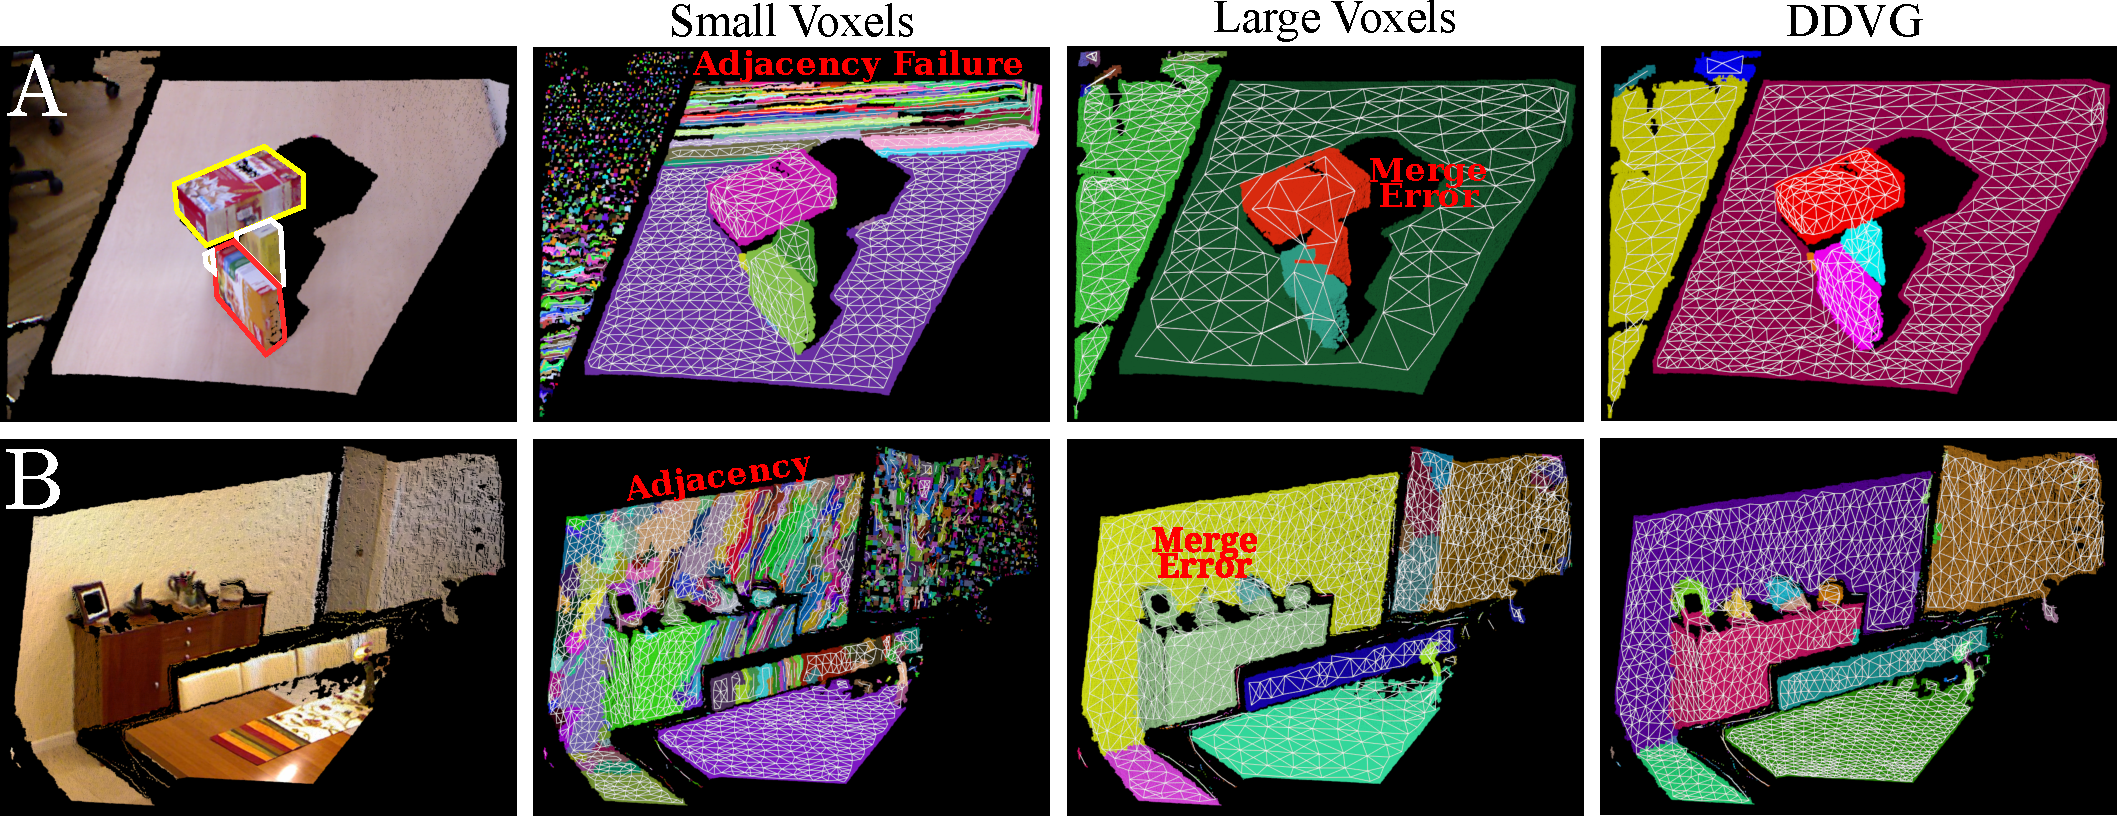
\includegraphics[width = \linewidth]{figures/CVPR2014/transform_results_v2}
\caption[Depth Adaptive Transform]{Two example point clouds \textbf{(A,B, left)} showing the need for the \gls{ddvg}. For better visibility outlines have been drawn around the boxes in A. Using \textit{Small Voxels} objects close to the camera can be segmented, but adjacency breaks down as the depth increases and the point density decreases. Using \textit{Large Voxels} corrects the adjacency graph in the background, but leads to objects being merged in the foreground due to the coarse resolution. Using \gls{ddvg}, the scale of the voxels gradually increases with distance from the camera -- adapting to the increased noise level and lower point density -- consequently adjacency is maintained and the segmentation of scenes with large depth variance is possible using fixed parameters. }
\label{fig:quantization_transform}
\end{figure}


\section{Locally Convex Connected Patches}
As an example of an application of supervoxels and the adjacency octree, we shall briefly present a segmentation method which breaks a supervoxel adjacency graph into meaningful segments by classifying whether an edge $e=(\vec p_i, \vec p_j)$ between two supervoxels is convex or concave. This classification is based on an \emph{\gls{ecc}}, which considers adjacent supervoxels with centroids at the positions $\vec x_1,\vec x_2$ and normals $\vec n_1, \vec n_2$. Whether the connection between these is convex or concave can be inferred from the relation of the surface normals to the vector joining their centroids - an overview of the this algorithm is given in Figure~\ref{fig:flow}.

\begin{figure}
\centering
  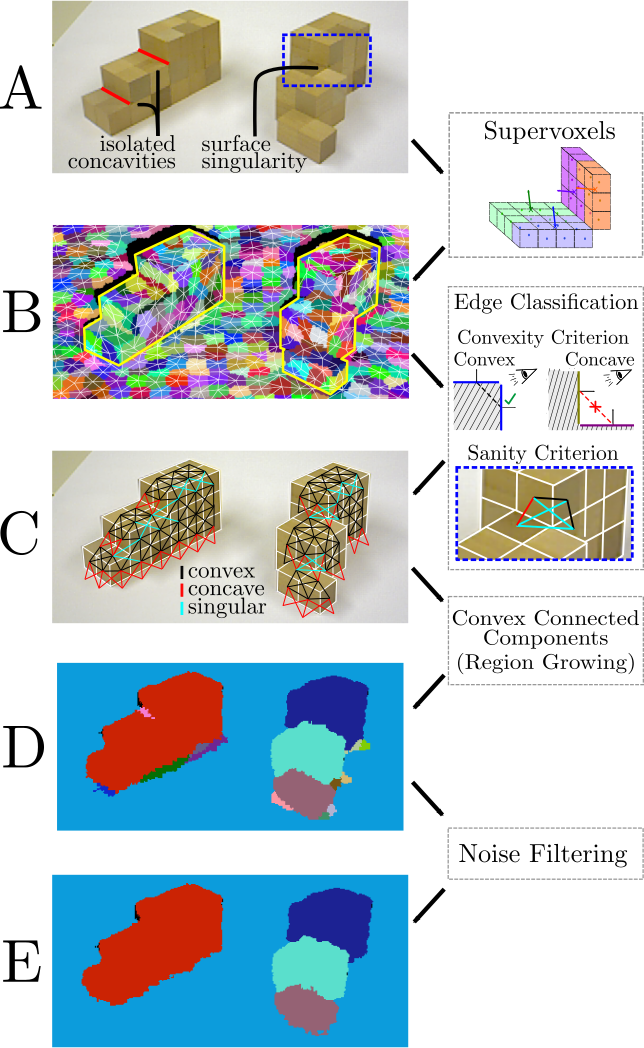
\includegraphics[width=0.8\linewidth]{figures/CVPR2014/flow_diagram}
    \caption[Flow Diagram of LCCP]{Flow diagram of the segmentation algorithm. \textbf{A)} RGB images corresponding to the point clouds of the scene. The red lines show two isolated concavities. The blue box shows an area with a surface singularity. \textbf{B)} Supervoxel adjacency graph. \textbf{C)} Model depicting the classified graph. Black lines denote convex connections, red lines concave ones and turquois lines singular connections (those, where two patches are connected only in a single point). \textbf{D)} Segmentation result; object labels are shown by different colors. \textbf{E)} Final result after noise filtering. The right column illustrates the supervoxel patches and the convexity and sanity criteria used for edge classification.}
  \label{fig:flow}
\end{figure}

The angle of the normals to the vector $\vec d = \vec x_1-\vec x_2$ joining the centroids can be calculated using the identity for the dot product $\vec a\cdot \vec b = |\vec a|\cdot |\vec b|\cdot \cos(\alpha)$ with $\alpha = \measuredangle(\vec a,\vec b)$. For \textit{convex} connections, $\alpha_1$ is smaller than $\alpha_2$ (see Fig.~\ref{fig:details}~A). This can be expressed as:
  \begin{equation*}
    \alpha_1 < \alpha_2 \Rightarrow \cos(\alpha_1) - \cos(\alpha_2) > 0 \Leftrightarrow \vec {n_1}\cdot \hat d - \vec {n_2}\cdot \hat d > 0,
  \end{equation*}
where $\hat d = \frac{\vec{x_1}-\vec{x_2}}{||\vec{x_1}-\vec{x_2}||}$. Similarly, for a \textit{concave} connection we get:
  \begin{equation*}
    \alpha_1 > \alpha_2 \Leftrightarrow \vec {n_1}\cdot \hat d - \vec {n_2}\cdot \hat d < 0.
  \end{equation*}
Note that these operations are commutative, thus the choice of which patch is $\vec x_1$, does not change the result. Also the criterion is still valid if the $\vec x_i$ are displaced, as long as they stay within the surface.

To compensate for noise in the RGB-D data, a bias is introduced to treat concave connections with very similar normals, that is
\begin{align*}
  \beta = \measuredangle(\vec n_1,\vec n_2) = |\alpha_1-\alpha_2| = \cos^{-1}(\vec{n_1}\cdot \vec{n_2}) < \beta_\text{Thresh}~,
\end{align*}
as convex, since those usually represent flat surfaces. Depending on the value of the \textit{concavity tolerance threshold} $\beta_\text{Thresh}$, concave surfaces with low curvature are seen as convex and thus merged in the segmentation. This behavior may be desired to ignore small concavities. We set:
\begin{align}
  \text{CC}_b(\vec p_i, \vec p_j) :=
  \left\{\begin{array}{lc}
          \text{true} & \left(\vec {n_1} - \vec {n_2} \right) \cdot \hat d  > 0~ \lor~ (  \beta < \beta_\text{Thresh} )\\
            \text{false} & \text{otherwise.}\\
          \end{array} \right.
  \label{eqn:CC}
\end{align}

where the variable $CC_b$ defines the {\em basic convexity criterion}. However, local errors in the feature estimation caused by noise in the data can propagate very easily, potentially leading to errors in the resulting segmentation. This also makes the recognition of small concavities harder, as subtle features are more sensitive to noise. To improve on this we also include neighborhood information in the classification of edges: For a convex edge $e=(\vec p_i, \vec p_j)$, we require that there exists a common neighbor $\vec p_c$ of $\vec p_i$ and $\vec p_j$ that has a convex connection to both.

Thus we define \textit{extended convexity} $CC_e$:
\begin{align}
  \begin{aligned}
   \text{CC}_e (\vec p_i, \vec p_j) = \text{CC}_b(\vec p_i, \vec p_j) \land \text{CC}_b(\vec p_i, \vec p_c) \\ \land \text{CC}_b(\vec p_j, \vec p_c)
  \end{aligned}
\end{align}

With extended convexity, more evidence is necessary for a connection to be labeled as convex. 

As in \gls{vccs}, clusters are found in \gls{lccp} using a region growing process: First, an arbitrary seed supervoxel is chosen and labeled. This label is then propagated over the graph with a depth search that is only allowed to grow over convex edges. Once no new supervoxel can be assigned to the segment, we choose a new seed supervoxel that has not been labeled and propagate the new label as before, repeating the process until all supervoxels have been labeled. Note that all of the criteria in \gls{lccp} are commutative, so the output of the region growing does not depend on the choice of the seeds.

\section{Experimental Results}
\subsection{Datasets}
In the following sections we present quantitative results for \gls{vccs} and \gls{lccp}. We compare both to state-of-the-art methods on the \textit{NYU Indoor Dataset}\cite{Silberman:ECCV12} and \textit{Object Segmentation Database}\cite{Richtsfeld:IROS12}. Before giving results, we shall first describe the datasets as well as the procedure for scoring results using 2D ground-truth.

\subsubsection{Object Segmentation Database (OSD)}
The \textit{Object Segmentation Database} (OSD-v0.2) was proposed by Richtsfeld \textit{et al.}\cite{Richtsfeld:IROS12} in 2012. It consists of 111 cluttered scenes of objects on a table, taken with close proximity to the pictured objects. The scenes contain multiple objects, which have mostly box-like or cylindrical shape, with partial and full occlusions and heavy clutter in 2D as well as 3D. Importantly, most objects in the data set are \textit{simple}, that is, consist of only a single part. This makes the ground-truth data relatively non-ambiguous.

\begin{figure}
 \centering
 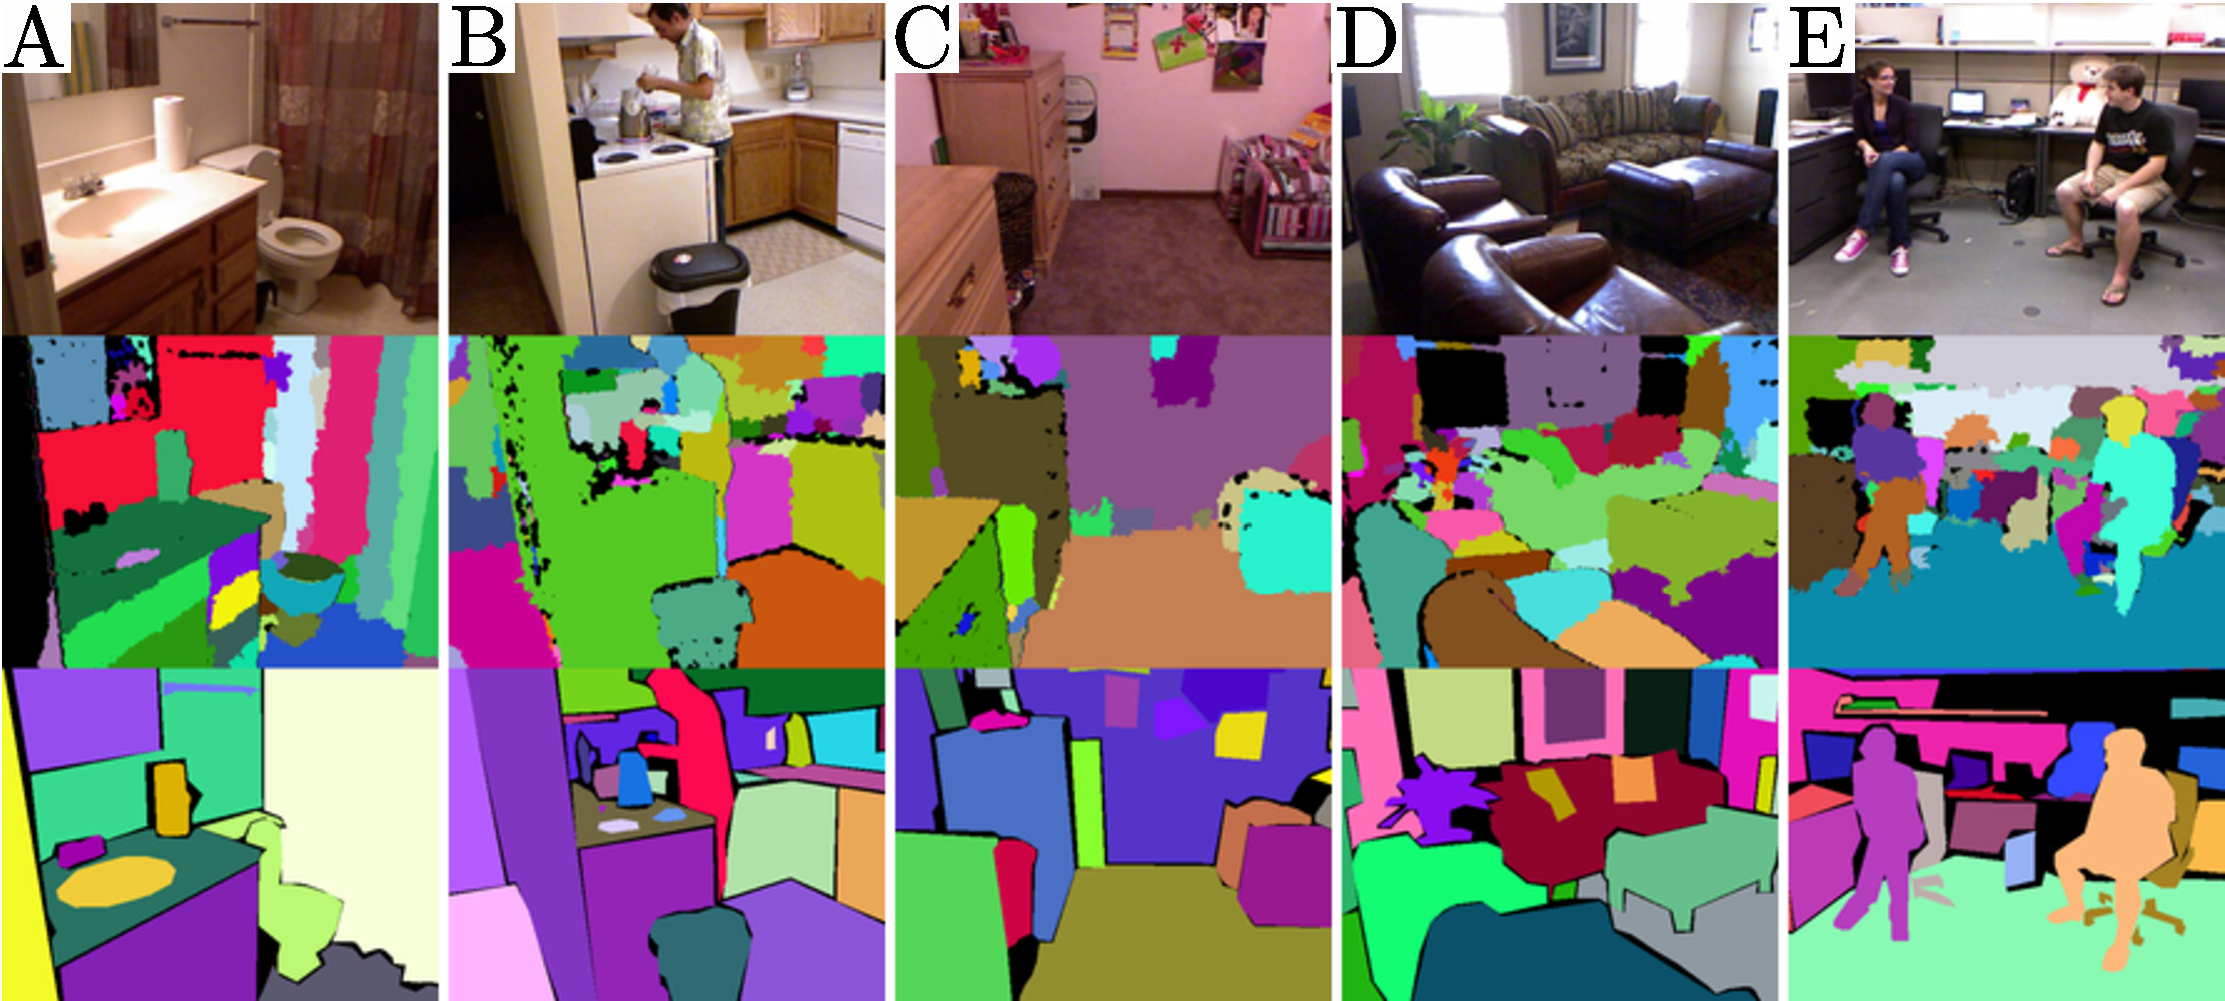
\includegraphics[width=1\linewidth]{figures/CVPR2014/nyu_examples.pdf}
 \caption[NYU Dataset Examples]{Example results for scenes from the NYU dataset using unsmoothed depth. Black areas indicate missing depth. Top row: rgb images. Mid. row: segmentation result. Bottom row: ground truth. Parameters A-C: $R_{voxel}=0.0075$, $R_{seed}=0.03$ and $\beta_\text{Thresh}=8^\circ$. Parameters D-E: $R_{voxel}=0.01$, $R_{seed}=0.04$ and $\beta_\text{Thresh}=10^\circ$ (identical to quantitative results, see Tab. \ref{tab:res_lccp_nyu}).}
 \label{fig:nyu_examples}
\end{figure}

\subsubsection{NYU Indoor Dataset (NYU)}
The \textit{NYU Indoor Dataset}\footnote{\url{http://cs.nyu.edu/~silberman/datasets/nyu_depth_v2.html}} (NYUv2) from Silberman \textit{et al.}\cite{Silberman:ECCV12} is a large and complex dataset, consisting of 1449 cluttered indoor scenes. The data consists of pairs of aligned RGB and depth images, along with human annotated densely labeled ground truth. The images were captured in diverse indoor scenes, and present many difficulties for segmentation algorithms such as varied illumination and many small similarly colored objects. Examples of typical scenes are shown in Figure~\ref{fig:ExampleSegmentations}. One main difficulty presented by the dataset is that the distance to objects from the camera is quite large in the dataset. This results in significant depth quantization artifacts as well as few data points for many objects. Additionally, depth is often missing for extensive portions of many of the images, due to limitations of the Kinect sensor (e.g. reflective, transparent surfaces - windows are especially problematic). Silberman \textit{et al.} attempt to correct for these errors using a hole filling algorithm (smoothdepth), which estimates depth for missing areas based on the scheme from Levin \textit{et al.}\cite{Levin2004}.

%------------------------------------------------------------------------
\begin{figure}
\begin{center}
%\fbox{\rule{0pt}{2.4in} \rule{0.9\linewidth}{0pt}}
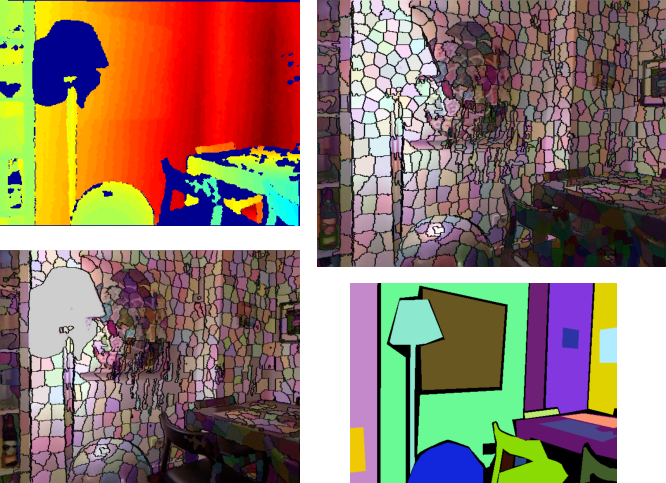
\includegraphics[width=0.9\linewidth]{figures/CVPR2013/BackTo2D.pdf}
\end{center}
   \caption[2D Hole Filling]{Example of hole-filling for images after returning from voxel-cloud to the projected image plane. Depth data, shown in the top left, has holes in it, shown as dark blue areas (here, due to the lamp interfering with the Kinect). The resulting supervoxels do not cover these holes as shown in the bottom left, since the cloud has no points in them. To generate a complete 2D segmentation, we fill these holes in using the SLIC algorithm, resulting in a complete segmentation, seen in the top right. The bottom right shows human annotated ground truth for the scene. }
\label{fig:ReturnToPlane}
\end{figure}
%------------------------------------------------------------------------

%------------------------------------------------------------------------
%\begin{figure}
%\begin{center}
%\includegraphics[width=1.01\linewidth]{figures/CVPR2013/Multiview.pdf}
%\end{center}
%   \caption[Supervoxels from Multiple Views]{Over-segmentation of a cloud from the RGB-D scenes dataset\cite{RGBDDataset}. The cloud is created by aligning 180 Kinect frames, examples of which are seen on the left side. The resulting cloud has over 3 million points, which reduces to 450k points at ${R}_{voxel}=0.01m$ and 100k points with ${R}_{voxel}=0.02m$. Over-segmentation of these take 6 and 1.5 seconds, respectively (including voxelization).}
%\label{fig:MultiViewCloud}
%\end{figure}
%------------------------------------------------------------------------

%------------------------------------------------------------------------
\begin{figure}
\begin{center}
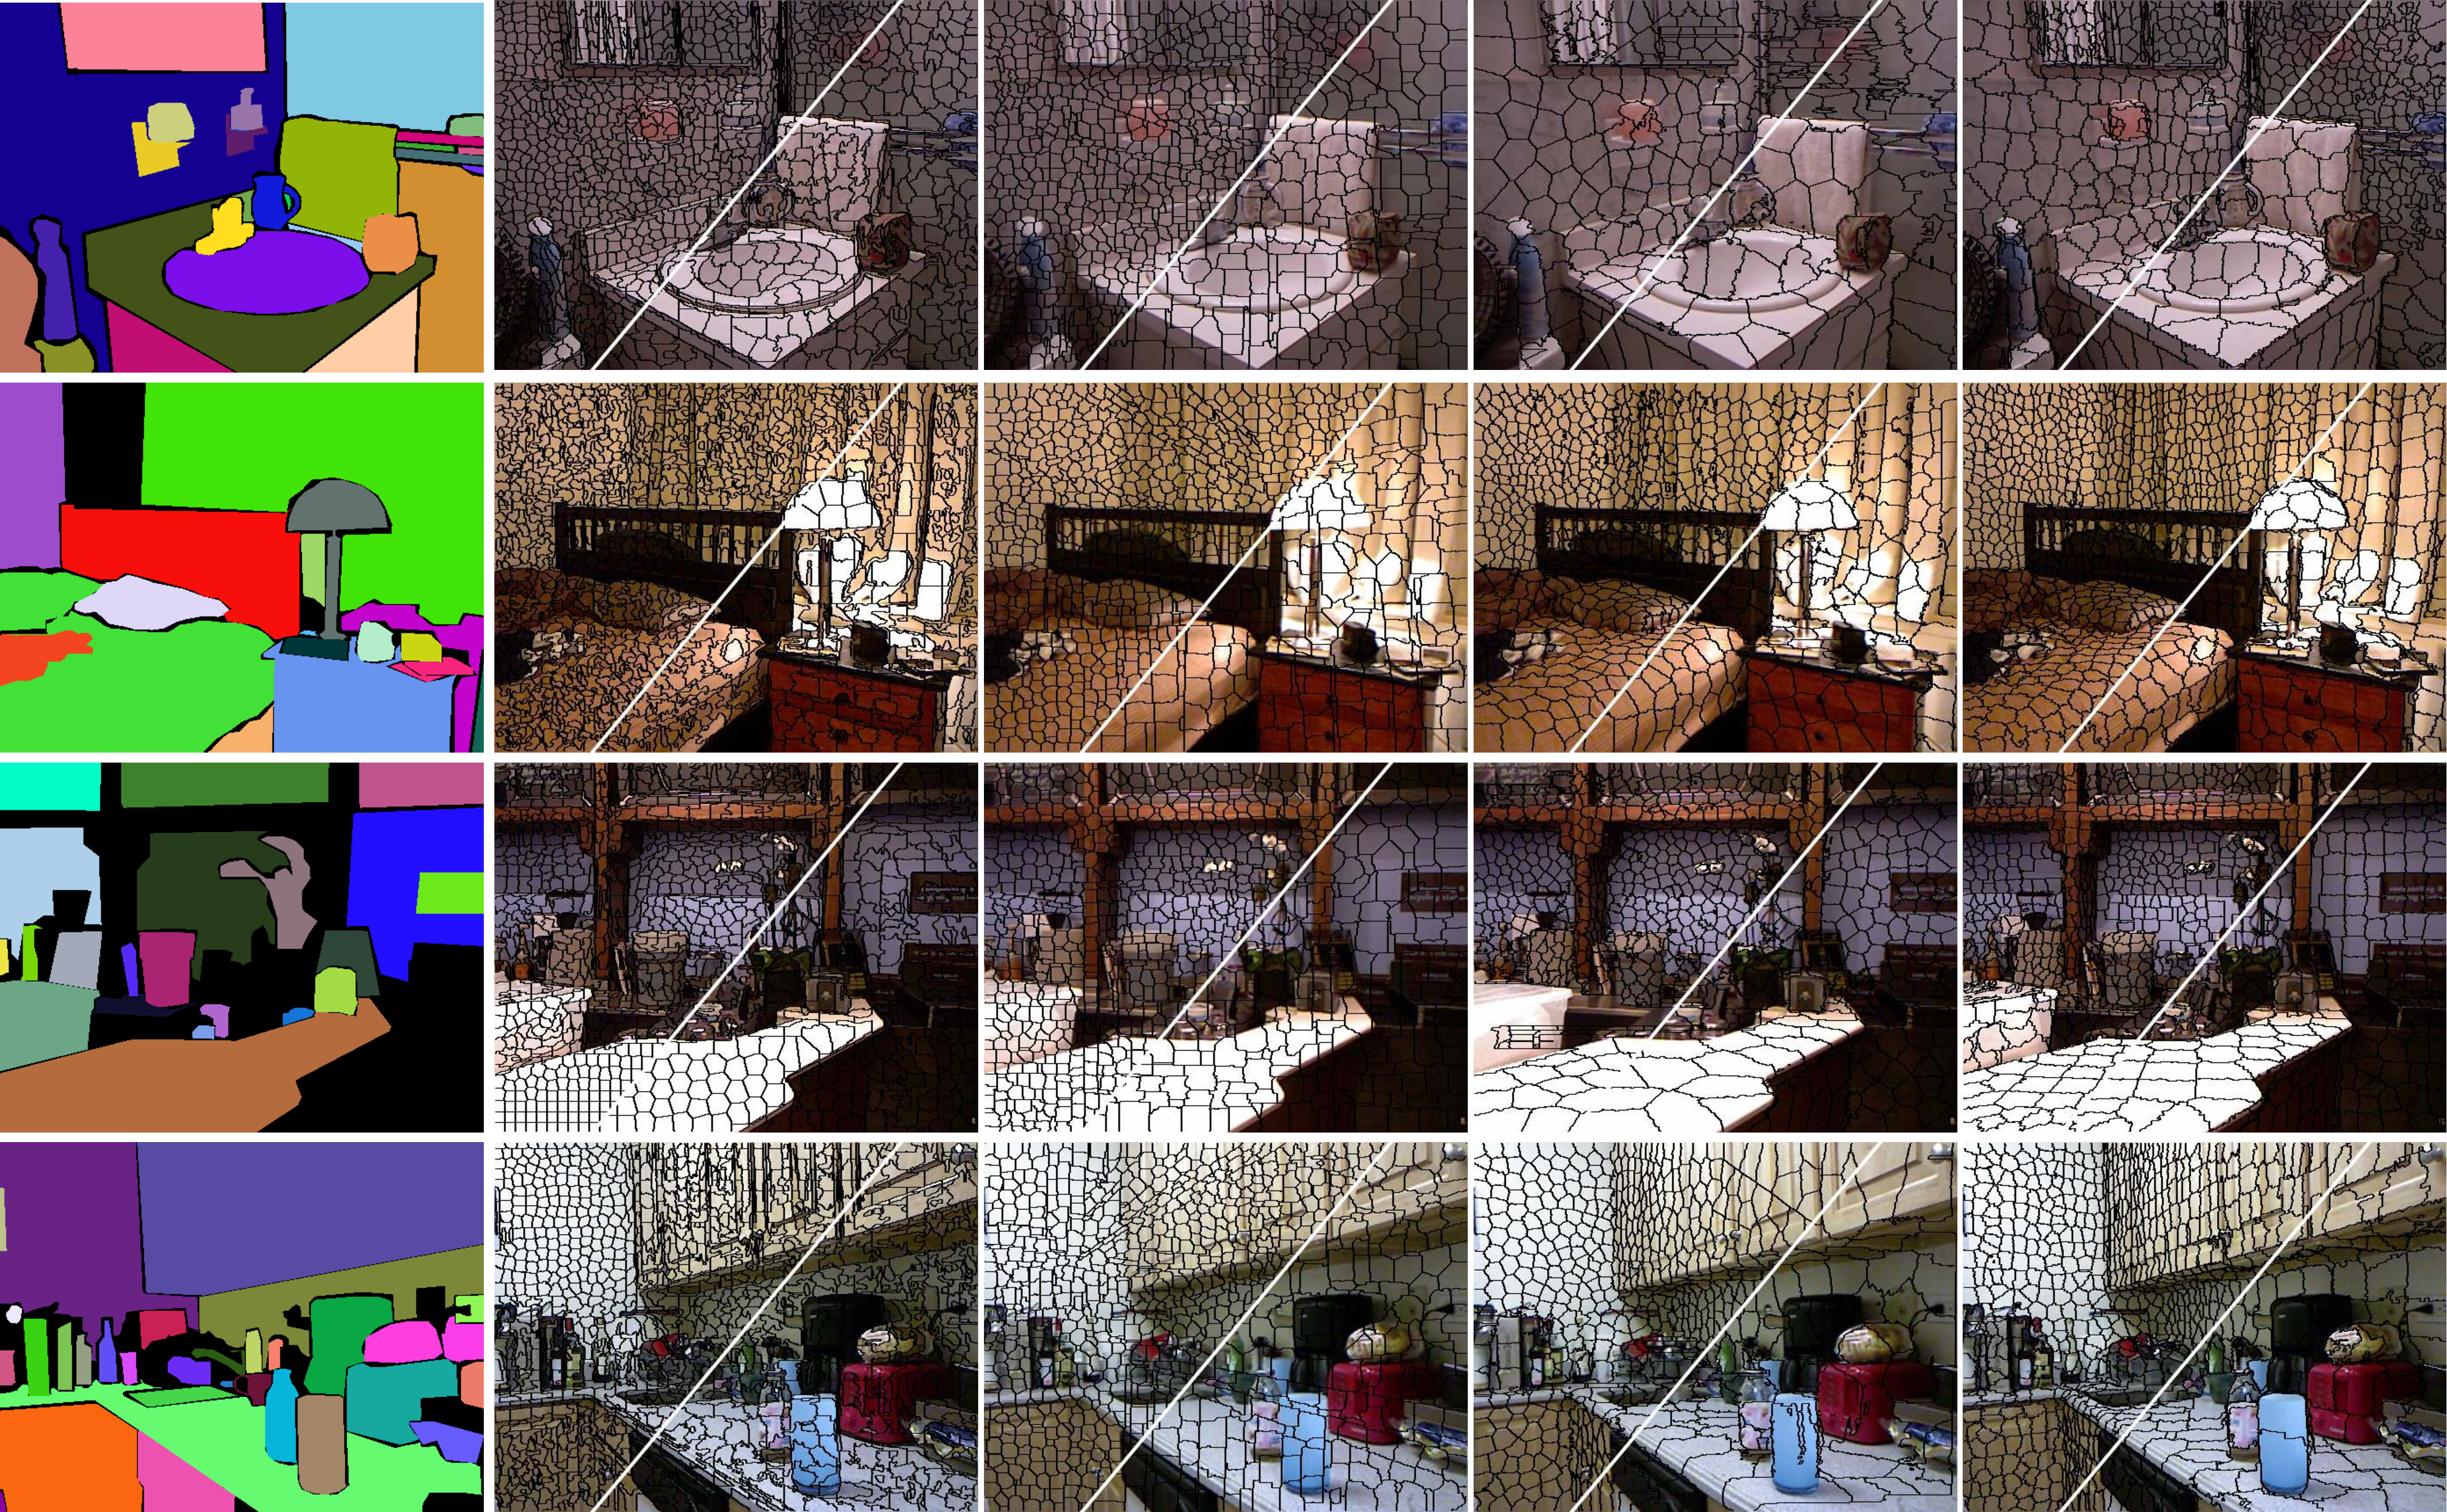
\includegraphics[width=1.01\linewidth]{figures/CVPR2013/Comparison_Segmentation_Small.pdf}
\end{center}
   \caption[Superpixel Comparison]{Examples of under-segmentation output. From left to right- ground truth annotation, SLIC, GCb10, DASP, and \gls{vccs}. Each is shown with two different superpixel densities.}
\label{fig:ExampleSegmentations}
\end{figure}
%------------------------------------------------------------------------

\subsubsection{Returning to the Projected Plane}
RGB+D sensors produce what is known as an organized point cloud- a cloud where every point corresponds to a pixel in the original RGB and depth images. When such a cloud is voxelized, it necessarily loses this correspondence, and becomes an unstructured cloud which no longer has any direct relationship back to the 2D projected plane. As such, in order to compare results with existing 2D methods we were forced to devise a scheme to apply supervoxel labels to the original image. 

To do this, we take every point in the original organized cloud and search for the nearest voxel in the voxelized representation. Unfortunately, since there are blank areas in the original depth image due to such factors as reflective surfaces, noise, and limited sensor range, this leaves us with some blank areas in the output labeled images. To overcome this, we fill in any large unlabeled areas using the SLIC algorithm. This is not a significant drawback, as the purpose of the algorithm is to form supervoxels in 3D space, not superpixels in the projected plane, and this hole-filling is only needed for comparison purposes. Additionally, the hole filling actually makes our results worse, since it does not consider depth, and therefore tends to bleed over some object boundaries that were correctly maintained in the supervoxel representation. An example of what the resulting segments look like before and after this procedure are shown in Figure~\ref{fig:ReturnToPlane}. 

\subsection {Supervoxels}
\label{sec:Evaluation}
In order to evaluate the quality of supervoxels generated by \gls{vccs}, we performed a quantitative comparison with three state-of-the-art superpixel methods using publicly available source code. 
We selected the two 2D techniques with the highest published performance from a recent review \cite{SLICCompared}: a graph based method, GCb10 \cite{SuperpixelsSupervoxels}\footnote{\url{http://www.csd.uwo.ca/~olga/Projects/superpixels.html}}, and a gradient ascent local clustering method, SLIC \cite{SLICCompared}\footnote{\url{http://ivrg.epfl.ch/supplementary_material/RK_SLICSuperpixels/index.html}}.
Additionally, we selected another method which uses depth images, DASP\cite{DASP}\footnote{\url{https://github.com/Danvil/dasp}}.
Examples of over-segmentations produced by the methods are given in Figure~\ref{fig:ExampleSegmentations}.
%------------------------------------------------------------------------
\begin{figure}
\begin{center}
%\includegraphics[width=0.8\linewidth,type=eps,ext=.eps,read=.eps]{Figures/boundary}
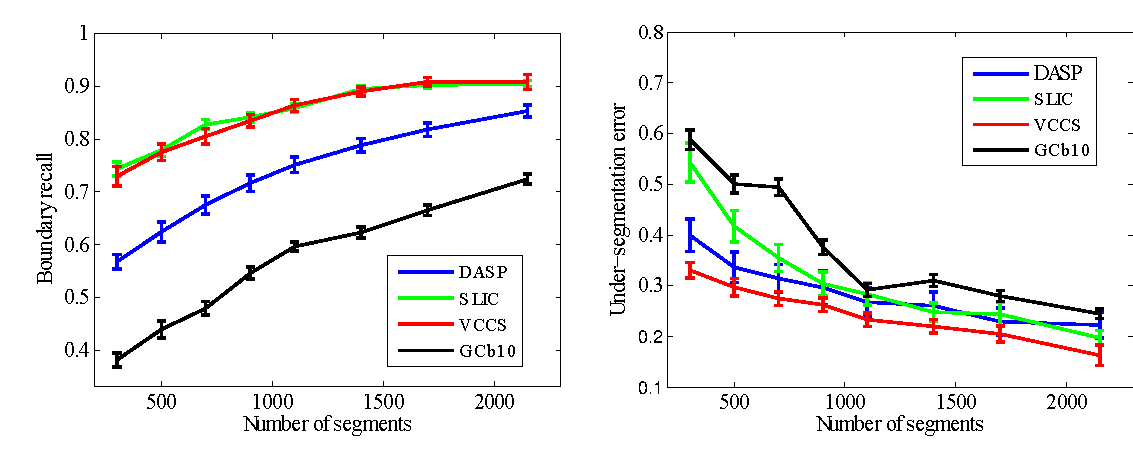
\includegraphics[width=0.95\linewidth]{figures/CVPR2013/Performance.pdf}
\end{center}
   \caption[Boundary Recall \& Undersegmentation Error]{Boundary recall and under-segmentation error for SLIC, GCb10, DASP, and \gls{vccs}.}
\label{fig:BoundaryRecall}
\label{fig:UndersegError}
\end{figure}
%------------------------------------------------------------------------
\subsubsection{Object Boundary Adherence}
The most important property for superpixels is the ability to adhere to, and not cross, object boundaries. To measure this quantitatively, we have used two standard metrics for boundary adherence- boundary recall and under-segmentation error\cite{Turbopixels, SuperpixelsSupervoxels}. Boundary recall measures what fraction of the ground truth edges fall within at least two pixels of a superpixel boundary. High boundary recall indicates that the superpixels properly follow the edges of objects in the ground truth labeling. The results for boundary recall are given in Figure~\ref{fig:BoundaryRecall}. As can be seen, \gls{vccs} and SLIC have the best boundary recall performance, giving similar results as the number of superpixels in the segmentation varies. 

Under-segmentation error measures the amount of leakage across object boundaries. For a ground truth segmentation with regions $g_1,...,g_M$, and the set of superpixels from an over-segmentation, $s_1,...s_K$, under-segmentation error is defined as 
\begin{equation}
\label{eqn:UndersegError}
{E}_{useg}=\frac{1}{N} \left[ \sum_{i=1}^{M}{\left(\sum_{s_j \mid s_j \cap g_i}{|s_j|}\right)-N} \right],
\end{equation}
where $s_j \mid s_j \cap g_i$ is the set of superpixels required to cover a ground truth label $g_i$, and $N$ is the number of labeled ground truth pixels. A lower value means that less superpixels violated ground truth borders by crossing over them. Figure~\ref{fig:UndersegError} compares the four algorithms, giving under-segmentation error for increasing superpixel counts. \gls{vccs} outperforms existing methods for all superpixel densities. 

\subsubsection{Time Performance}
As superpixels are used as a preprocessing step to reduce the complexity of segmentation, they should be computationally efficient so that they do not negatively impact overall performance. To quantify segmentation speed, we measured the time required for the methods on images of increasing size (for the 2D methods) and increasing number of voxels (for \gls{vccs}). All measurements were recorded on an Intel Core i7 3.2Ghz processor, and are shown in Figure~\ref{fig:SegmentationSpeed}. \gls{vccs} shows performance competitive with SLIC and DASP (the two fastest superpixel methods in the literature) for voxel clouds of sizes which are typical for Kinect data at ${R}_{voxel}=0.008m$ (20-40k voxels). It should be noted that only \gls{vccs} takes advantage of multi-threading (for octree, kd-tree, and FPFH computation), as there are no publicly available multi-threaded implementations of the other algorithms.  

%------------------------------------------------------------------------
\begin{figure}
\begin{center}
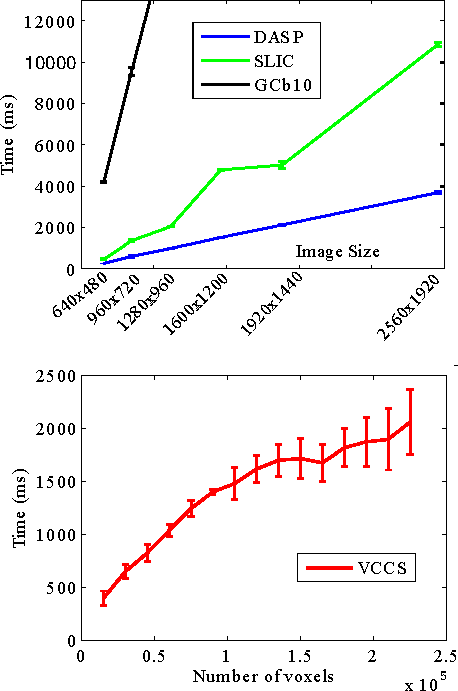
\includegraphics[width=0.95\linewidth]{figures/CVPR2013/Speed.pdf}
\end{center}
   \caption[Segmentation Speed]{Speed of segmentation for increasing image size and number of voxels. Use of GCb10 rapidly becomes unfeasible for larger image sizes, and so we do not adjust the axes to show its run-time. The variation seen in \gls{vccs} run-time is due to dependence on other factors, such as ${R}_{seed}$ and overall amount of connectivity in the adjacency graphs.}
\label{fig:SegmentationSpeed}
\end{figure}
%------------------------------------------------------------------------

\subsection{Locally Convex Connected Patches}

We compare segments found using \gls{lccp} against ground truth using three standard measures: \textit{Weighted Overlap} (WOv), which is a summary measure proposed by Silberman \textit{et al.} \cite{Silberman:ECCV12}, as well as \textit{false negative} ($fn$) and \textit{false positive} ($fp$) scores from \cite{Ritter2012} and \textit{over-} ($F_{os}$) and \textit{under-segmentation} ($F_{us}$) from \cite{Richtsfeld:IROS12}.

\begin{figure}
 \centering
 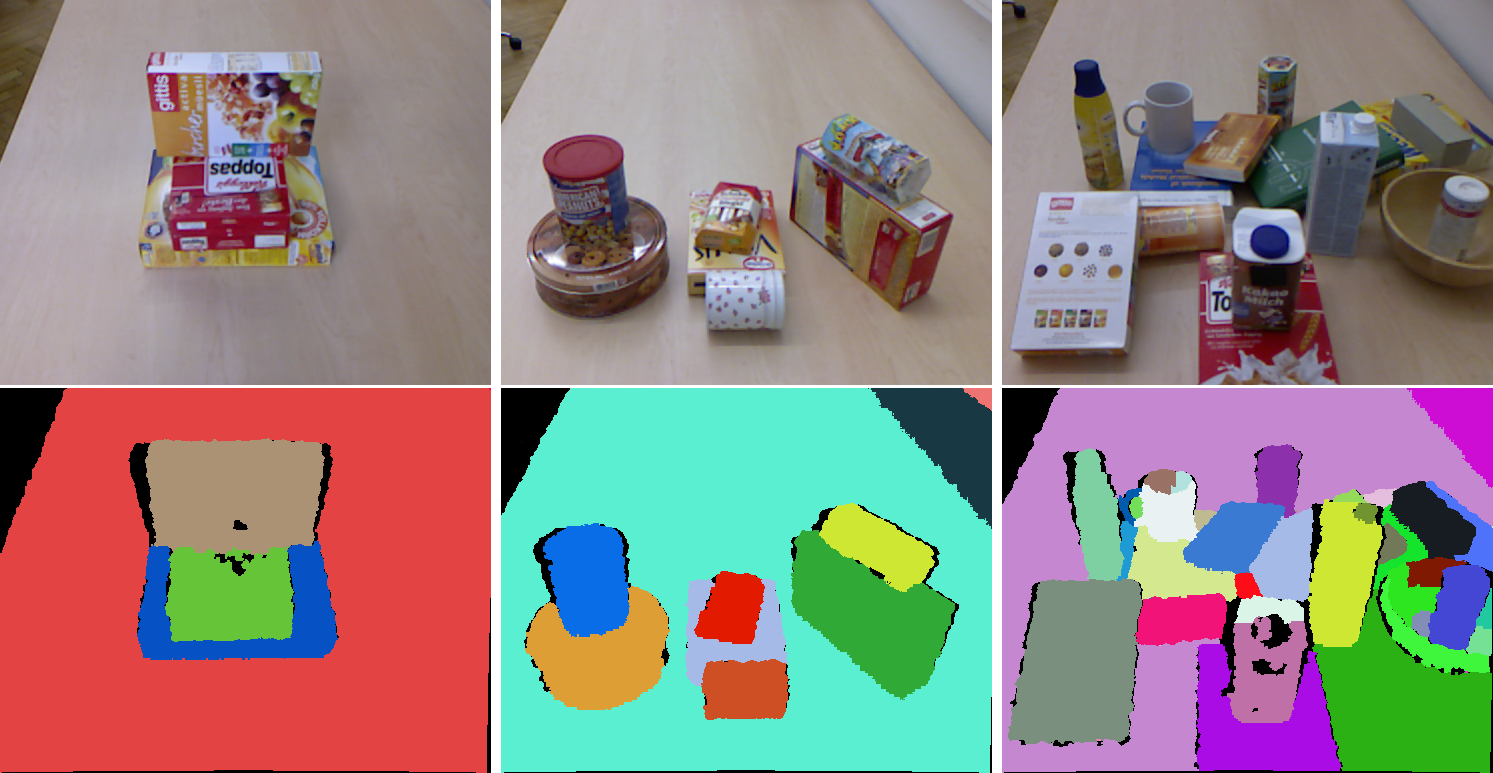
\includegraphics[width=1\linewidth]{figures/CVPR2014/osd_examples}
 \caption[OSD Dataset Examples]{ Example results for the OSD dataset. Points beyond a distance of 2m were cropped for visualization. Parameters: $R_{voxel}=0.005$, $R_{seed}=0.02$, $\beta_\text{Thresh}=10^\circ$.  }
 \label{fig:OSD_results}
\end{figure}

%%%%%%%%%%%%%%%%%%%%%%%%%%%%%%%%%%%%%%%%%%%%%%%%%%%%%%%%%%%%%%%%%%%%%%%%%%%%%%%%%%%%%%%%%%%%
 \begin{table*}[!ht]
   \small
   \centering
    \begin{tabular}{c||c||c||cc||cc||c||c}
    \multirow{2}{*}{Method} & Learned & WOv     & \multicolumn{2}{c||}{$fp$} & \multicolumn{2}{c||}{$fn$} & $F_{os}$ & $F_{us}$ \\ \cline{3-9}
    ~                       & Features & Mean   & Mean  & SD     & Mean  & SD    & Mean   & Mean   \\ \hline\hline
    LCCP            &  NO LEARNING & 88.7\% &  4.8\% & 2.6\%  & 8.3\% & 8.7\% & 7.4\%  & 4.7\%  \\ \hline
    Richtsfeld~\cite{Richtsfeld:IROS12}  & RGB-D,Texture,Geometry & -      & -          & -      & -     & -     & 4.5\%  & 7.9\%  \\ \hline
    {\"U}ckermann~\cite{Ritter2012} & NO LEARNING & -      & 1.9\% & 3.3\%  & 7.8\% & 7.3\% & -      & -      \\ \hline
    \end{tabular}
    \caption[Segmentation Results on OSD Dataset]{Comparison of different segmentation methods on the OSD dataset using weighted overlap \textit{WOv} (the higher, the better), false positives \textit{$f_p$}, false negatives \textit{$f_n$}, as well as over- and under-segmentation \textit{$F_{os}$} and \textit{$F_{us}$} (the lower, the better). LCCP results were produced with voxel resolution $R_{voxel} = 0.005$, seed resolution $R_{seed} = 0.02$ and concavity tolerance angle $\beta_\text{Tresh}=10^\circ$.}
    \label{tab:res_stat}
\end{table*}

The qualitative examples from the OSD dataset (Fig.~\ref{fig:OSD_results}) show that \gls{lccp} performs very well in the segmentation of cluttered scenes. The object separation can be intuitively understood: all objects present in the scenes are separated by concave boundaries, i.e. a line connecting neighboring surfaces of two different objects always travels through ``air''. This is also true for the boundary between an object and the supporting surface. As a consequence, objects that have a convex shape are correctly captured as one segment and separated from the other objects. Hollow objects (bowls, cups etc.) can be observed to show multiple segments inside, because the orientation of surface normals changes strongly on these concave surfaces. The quantitative results (Table~\ref{tab:res_stat}) demonstrate that the approach is able to compete with state-of-the-art methods in the task of segmenting cluttered scenes with 'single-part' objects. 

\begin{table*}
  \centering
  \begin{tabular}{c|c|c|c}
%   \textbf{Overlap} & \textbf{Weighted Overlap} & \textbf{oversegmentation} & \textbf{undersegmentation} \\
  Method & Learned Features & Depth Data  & WOv\\ \hline \hline
  \multirow{2}{*}{LCCP} & NO LEARNING & depth & 53.6\% \\ \cline{2-4}
                                           & NO LEARNING & smoothdepth & 53.8\% \\ \hline
  LCCP + ext. convexity & NO LEARNING & smoothdepth &  57.6\% \\ \hline \hline
  \multirow{4}{*}{Silberman \textit{et al.}\cite{Silberman:ECCV12}} & RGB  & - &  50.3\% \\ \cline{2-4}
                                           & Depth & both  & 53.7\% \\ \cline{2-4}
                                           & RGB-D & both  & 60.1\% \\ \cline{2-4}
                                           & RGB-D + Support + Structure classes & both & 61.1\% \\ \hline \hline
  \multirow{2}{*}{Gupta \textit{et al.}\cite{Gupta:CVPR2013}} & gPb-ucm Gradients (from \cite{Arbelaez:PAMI2011}) & - &  55.0\% \\ \cline{2-4}
                                           & gPb-ucm + Depth + Concavity Gradients & both & 62.0\% \\ \hline
  \end{tabular}
  \caption[Comparison of NYU Dataset Results]{Comparison of different segmentation methods on the NYU dataset using weighted overlap \textit{WOv}. \gls{lccp} results were produced with voxel size $R_{voxel} = 0.01$, seed size $R_{seed}=0.04$ and concavity tolerance angle $\beta_\text{Tresh}=10^\circ$.}
  \label{tab:res_lccp_nyu}
\end{table*}

Example scenes in Fig.~\ref{fig:nyu_examples} show that the \gls{lccp} also works well on the real-world scenes from the NYU dataset. The quantitative results (Table~\ref{tab:res_lccp_nyu})\footnote{Updated results for \cite{Silberman:ECCV12} are available at \url{http://cs.nyu.edu/~silberman/datasets/nyu_depth_v2.html}.} show that our algorithm is able to produce good results on the challenging dataset. Despite being much simpler and without requiring learning on human annotated ground-truth, we compete with the approach from \cite{Silberman:ECCV12} when only depth information is used. Additionally, we still achieve 93\% of their score when comparing against the more complex feature spaces used in conjunction with learning-based algorithms. We should emphasize that our competitors do not aim for object parts but rather for ``whole object'' detections, specifically, those whole objects learned from this particular annotated ground truth. Conversely, our method establishes a general rule for object-ness that does not depend on this particular dataset, nor on the whims of a particular human annotator.

\section{Discussion}

In this Chapter we have presented several new concepts- the octree adjacency graph, supervoxels, a segmentation method which uses supervoxels, as well as a way to sequentially update an octree with new frames of data. Additionally, we have presented quantitative and qualitative results which demonstrate the usefulness of these techniques. In particular, \gls{lccp} has demonstrated the usefulness of a patch-based adjacency-graph interpretation of 3D Point Cloud data. The results we achieved stem from two core properties: the ability of supervoxels to efficiently encode local regions, and the usefulness of a 3D adjacency-graph in resolving situations which are ambiguous in a 2D representation.

In the next Chapter, we will use the octree model we have developed here as observations for particle filter tracking. We will demonstrate its effectiveness as the basis for correspondence association, and show how its preservation of voxels through occlusions allows us to track objects in a real-world application. Additionally, we shall use the supervoxels we presented here as the basis for dividing tracked models into strata, and show how this can be used to vastly improve the run-time performance of a tracker. 

%% Requires fltpage2 package
%%
% \begin{FPfigure}
% \includegraphics[width=\textwidth]{figures/fullpage}
% \caption[Short figure name.]{This is a full page figure using the FPfigure command. It takes up the whole page and the caption appears on the preceding page. Its useful for large figures. Harvard's rules about full page figures are tricky, but you don't have to worry about it because we took care of it for you. For example, the full figure is supposed to have a title in the same style as the caption but without the actual caption. The caption is supposed to appear alone on the preceding page with no other text. You do't have to worry about any of that. We have modified the fltpage package to make it work. This is a lengthy caption and it clearly would not fit on the same page as the figure. Note that you should only use the FPfigure command in instances where the figure really is too large. If the figure is small enough to fit by the caption than it does not produce the desired effect. Good luck with your thesis. I have to keep writing this to make the caption really long. LaTex is a lot of fun. You will enjoy working with it. Good luck on your post doctoral life! I am looking forward to mine. \label{fig:myFullPageFigure}}
% \end{FPfigure}
% \afterpage{\clearpage}

\begin{savequote}[75mm]
Optical Illusion is optical truth! ... In them is evidenced the living interaction of our inner nature with outer nature.
\qauthor{Johann Wolfgang von Goethe}
\end{savequote}

%For an example of a full page figure, see Fig.~\ref{fig:myFullPageFigure}.
\chapter{Model-Based Point Cloud Tracking}
\label{Chap:ModelBasedTracking}
\lettrine[lines=3, loversize=0.3]{\textcolor{Silver}N}{ow that we have established} a reduced, stable world model in which voxels persist through occlusions, the next step is to adapt the general framework of \gls{sbf} to track models within this 3D voxel world. For an introduction to the general framework of \gls{sbf}, we refer the reader to Appendix \ref{chap:SeqBayesEst}). In this Chapter we begin by presenting the basic framework of particle filter tracking in 3D point clouds, and show how point correspondences can be used to evaluate the particle filtering likelihood function.

While the correspondence approach is feasible for tracking single targets, it suffers from the same flaw as other approaches when extended to multiple targets \cite{MCMCPartFilt_05, ApproxMultiTrack_06,Koo_IROS2013, Breitenstein_ICCV2009} - it significantly increases the computational resources required. This increase is due to the need for more particles - due to assignment of particles to individual targets, a larger state space, or independent filters for each target. While there has been work addressing this problem by offloading processing to a GPU \cite{Choi_IROS2013}, in this work we take a different approach, and search for fundamental changes to the point cloud correspondence particle filter which can reduce computational complexity without affecting accuracy. 

This Chapter is organized as follows: First, in Section \ref{sec:PartFilt3d} we present a framework for particle filter tracking in point clouds using point correspondences. In Section \ref{sec:StratCorrSampling} we present the primary contribution of this Chapter; the use of a supervoxel-based stratified sampling approach to greatly reduce the computational complexity of point cloud correspondence particle filtering. Finally, in Section \ref{sec:ExperimentalResults} we will show that the approach allows performance (on a standard CPU) exceeding that which can be obtained on a recent GPU implementation \cite{Choi_IROS2013}. Furthermore, we shall present extensive quantitative experiments demonstrating the benefits of this approach, as well as show qualitative results from a real-world application. 

\section{Particle Filters in 3D}
\label{sec:PartFilt3d}
The underlying mechanics of 3D point cloud correspondence particle filtering remain the same as in Chapter \ref{Chap:VideoSegRelaxation}, and so we shall not discuss them extensively here; for a detailed introduction to the topic, we again refer the reader to \cite{Doucet2001} or \cite{SequentialMonteCarloMultitargetFiltering}. Rather, we shall only discuss the aspects that differentiate it - the models and how they are scored and propagated. The models here consist of point clouds, and the measurement function relies on point to point correspondence for scoring, rather than a global per-detection metric (such as a histogram distance, used in the 2D trackers of in Chapter \ref{Chap:VideoSegRelaxation}). The dynamic model uses real-world 3D coordinates which also include orientation, rather than 2D pixel coordinates in the image plane. The primary novelty of the approach we present here lies in how we score individual particle predictions using the measurement model. 

\subsection{Model Representation}
One of the main limitations of the 2D projected mask model discussed in Chapter \ref{Chap:VideoSegRelaxation} is that the masks of objects are not invariant to pose changes - in general, rotation of an object will change the shape of its mask and distribution of its color histogram. As we now have the ability to observe the full 3D shape of an object, we choose to represent objects as clusters of points which correspond to the exterior of the object. A visual representation of such a model is given in Figure \ref{fig:ModelExample}.

\begin{figure*}[!ht]
  \centering
  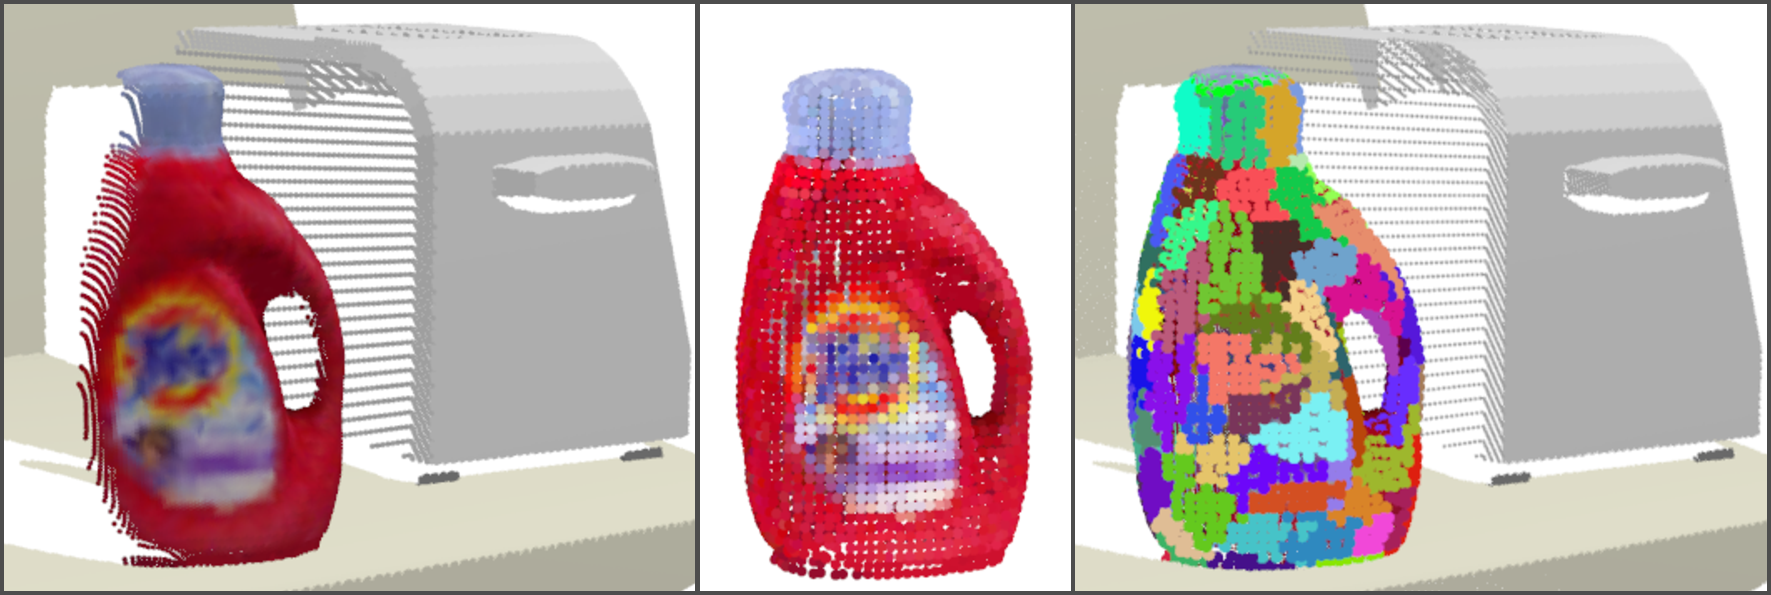
\includegraphics[width=1.0\textwidth]{figures/Tracking/TideModelSV.pdf}
  \caption[Example of data from ``Tide'' sequence.]{Example of data from ``Tide'' sequence. The left frame shows an example of the raw input cloud. Sampling effects from the synthetic RGB-D camera are visible in the quantization of points, especially on the edges of objects. The middle frame shows the voxelized model representation we use, while the right frame shows an example of supervoxel strata used for sampling with $R_{seed} = 0.07m$.}
  \label{fig:ModelExample}
\end{figure*}

Points for objects are stored in a model-centered reference frame (which we shall denote with superscript $^m$), with each point containing an XYZ position, an RGB color for the point, as well as a surface normal vector. That is, each point $p$ of the model $k$ consists of a nine-dimensional vector: 

\begin{equation} \label{eqn:point}
p^m_k = [x^m,y^m,z^m,R,G,B,n_x,n_y,n_z],
\end{equation}
 
 and a model for an object $O_k$ consists of a vector of $n_k$ such points $p^m$:
 
 \begin{equation} \label{eqn:model}
 O^m_k = [p^m_0 ... p^m_{n_k}].
\end{equation}

It is important to note that the points of an object model given above are model-relative - they must be transformed into the world coordinates in order to evaluate their fit to observations. This will be discussed further in the next Section.


\subsection{Dynamic Model}
\label{sec:Dynamic_model}
In the 2D tracker presented previously, the time-dependent state vector of a particle consisted of a position shift vector $\mathbf{p}_t=[p_x,p_y]$ and a velocity vector $\mathbf{v}_t=[v_x,v_y]$. The natural extension of this to 3D is to simply add a third $p_z$ and $v_z$ element to each. Of course we should note that the $x$ and$y$ dimensions here in our 3D representation are distinct from those in 2D, which represented pixel coordinates in the image plane. Here our positional coordinates represent real-world distances from a fixed origin (typically the camera ``pin-hole'' position). It is also important to note that coordinates in our 3D representation are originally in a continuous space - though we discretize them using the octree model discussed in the previous Chapter. For clarity, we shall simply denote coordinates in the world reference frame with no superscript.

While this straightforward extension gives us a reasonable 3D equivalent to our 2D tracked masks, we now have full 3D models, and so it makes sense to use a state vector which takes advantage of it. As such, we further extend the state vector for position and velocity to allow for rotations of the model around the object reference frame x-axis (roll - $\gamma$), y-axis (pitch - $\beta$), and z-axis (yaw - $\alpha$). This yields a position state vector for particle $j$ at time $t$ of 
\begin{equation} 
 \mathbf{x}^j_t = [d_x, d_y, d_z, \gamma, \beta, \alpha].
\end{equation}
Each object model is tracking using a set of $N$ such particles. We shall now generally omit the object variable $k$ in our notation for clarity. Even though we omit the $k$, the reader should assume that the following equations are for individual object models, and that we have a set of $N$ independent particles for each object.
Additionally, we have velocity state vector 
\begin{equation} 
 \mathbf{v}_t = [v_x, v_y, v_z, v_{\gamma}, v_{\beta}, v_{\alpha}],
\end{equation}
which is not tracked individually per particle, but rather as a whole for the model.

As before, motion is modeled using a constant velocity model in discrete time with a variable sampling period $\mathit{T}$, giving the dynamic model
\begin{equation} 
\mathbf{x}_t = \mathbf{x}_{t-1} + \mathit{T}\mathbf{v}_{t-1} + \mathbf{\omega} , 
\end{equation}
with noise vector $\mathbf{\omega}$ assumed to be zero mean Gaussian with fixed covariance.
Particle velocities are updated after weighting of individual particles using the measurement model, and are a weighted average of the change in position
\begin{equation} 
\label{Eqn:group_vel}
\mathbf{v}_t = \frac{1}{\mathit{T}N} \sum_{j=1}^{N} w_j (\mathbf{x}^j_{t} - \mathbf{x}^j_{t-1}), 
\end{equation}
where $w_j$ is the normalized weight for particle $j$. 

Tracking independent velocities for each particle doubles the dimensionality of the state-space, requiring a proportional increase in the number of particles. While the use of independent velocity states potentially helps in complicated tracking scenarios, in our experiments we were unable to observe any tangible benefit. Moreover, in order to avoid instability in the tracking results we needed to double the number of particles for a given noise level, doubling the processing time required. As such, we have chosen to use the above ``group-velocity'', and leave it to future work to investigate the possibility of independent velocity states.

\subsection{Measurement Model}
As points for the model are given in a model-centered frame of reference, we must transform them to the world frame them using a 3D affine transformation quaternion:
\begin{equation} \mathbf{B}^j = 
\begin{bmatrix}
 \cos{\alpha}\cos{\beta} & \cos{\alpha}\sin{\beta}\sin{\gamma} - \sin{\alpha}\cos{\gamma} & \cos{\alpha}\sin{\beta}\cos{\gamma} + \sin{\alpha}\sin{\gamma}  & d_x \\ 
\sin{\alpha}\cos{\beta} & \sin{\alpha}\sin{\beta}\sin{\gamma} + \cos{\alpha}\cos{\gamma} & \sin{\alpha}\sin{\beta}\cos{\gamma} - \cos{\alpha}\sin{\gamma}  & d_y \\ 
 -\sin{\beta} & \cos{\beta}\sin{\gamma} & \cos{\beta}\cos{\gamma} & d_z \\ 
 0 & 0 & 0 & 1
\end{bmatrix} \end{equation}
 which we use to transform the extended position vector for each point in the model:
\begin{equation} 
  p^m = [x^m,y^m,z^m,1],
\end{equation}
 yielding positions in the world frame for each of our $\eta$ model points for a particular particle $j$:
\begin{equation} 
  \begin{bmatrix}
    \mathbf{p}^j_1 \\
    \mathbf{p}^j_2 \\
    \vdots \\
    \mathbf{p}^j_\eta
  \end{bmatrix}
  \begin{bmatrix}
    [x_1,y_1,z_1,1]^\mathsf{T} \\
    [x_2,y_2,z_2,1]^\mathsf{T} \\
    \vdots    \\
    [x_\eta,y_\eta,z_\eta,1]^\mathsf{T}
  \end{bmatrix}
  =
  \begin{bmatrix} 
    \mathbf{B}^j & 0 & \ldots & 0 \\
    0 & \mathbf{B}^j & \ldots &  0 \\
    \vdots & \vdots & \ddots & \vdots \\
    0 & 0 & \ldots & \mathbf{B}^j 
  \end{bmatrix} 
  \begin{bmatrix}
    [x^m_1,y^m_1,z^m_1,1]^\mathsf{T} \\
    [x^m_2,y^m_2,z^m_2,1]^\mathsf{T} \\
    \vdots    \\
    [x^m_\eta,y^m_\eta,z^m_\eta,1]^\mathsf{T}
  \end{bmatrix}.
\end{equation}

Once we have our transformed points, we then must establish correspondences between each particle's model points and a world point. This is done so that we may score how well a particular particle matches the current world model observation. That is, for each transformed point $\mathbf{p}^j_{1\dotso \eta}$, we select corresponding point $\mathbf{p}^*$ in the observation which has minimal spatial distance. To find these correspondences, we first compute a KD-tree in the spatial dimensions for the world model points. This allows us to efficiently search for the nearest point to each transformed point. We create this tree for the world model rather than the transformed model (even though the former has more points) as there is only one world, but many particles and models. Computing it for the models would require a KD-tree for each particle in each model. Additionally, computing it for the world allows us to take advantage of sampling strategies (discussed in the next Section) which significantly reduce our run-time complexity. 

Once we have selected (with replacement) an observed point correspondence for each model point, we must calculate an un-normalized weight $\tilde{w}^j$ corresponding to the similarity of the transformed points to the world observation. This is accomplished   by summing the individual correspondence scores computed using weighted distance in world-, color-, and normal-space:
\begin{equation} \label{eqn:distance}
  \tilde{w}^j = \sum_{1}^{\eta} \frac{1}{1 + \frac {\mu \lVert \mathbf{p}^j_{xyz} - \mathbf{p}^*_{xyz} \rVert} {R_{voxel}} +  \frac{\lambda D_c(p^j_{RGB},p^*_{RGB})}{m} +   \epsilon \lVert \mathbf{p}^j_{n_x n_y n_z} - \mathbf{p}^*_{n_x n_y n_z} \rVert}, 
\end{equation}
where we follow the convention given in Section\ref{subsec:Features}. That is, $\mu$, $\lambda$, and $\epsilon$ are weighting constants, $D_c$ is euclidean distance in HSV space, and $m$ is a normalizing constant. We do not normalize normals, as they are already unit vectors. In our experiments we typically set the weighting factors to $\mu=1$, $\lambda=2$, $\epsilon=1$, as this balances the scoring between color and geometric shape, and found experimentally that it produced consistently good tracking results. The calculated particle weights $\tilde{w}^j$ are then normalized, and a final state estimate can be computed by taking the weighted average of all particles
\begin{equation} 
\mathbf{x}_t = \sum_{j=1}^{N} w_j \mathbf{x}^j_{t}, 
\end{equation}
and the group-velocity can be computed using Equation~\ref{Eqn:group_vel}.


\section{Stratified Correspondence Sampling}
\label{sec:StratCorrSampling}
\begin{figure}[]
  \centering
  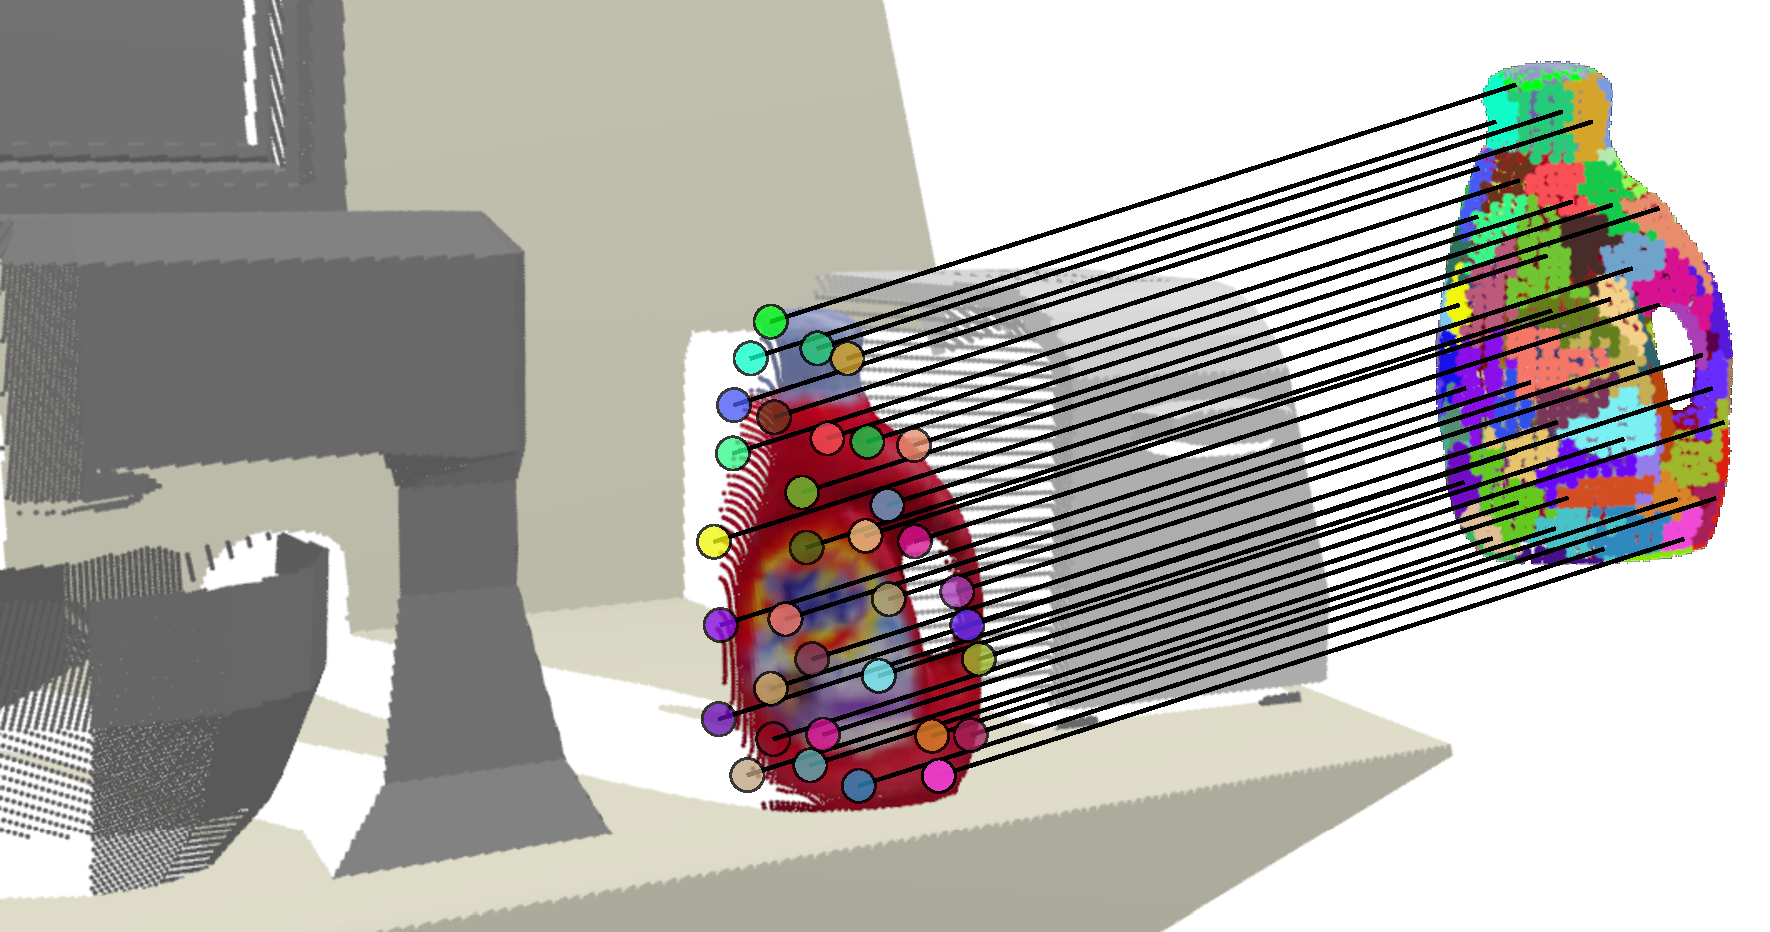
\includegraphics[width=\textwidth]{figures/Tracking/StratifiedCorrespondences.pdf}
  \caption[Stratified Correspondence Matching]{The model is divided into strata (shown as separate colors), and a random point is selected from each stratum for correspondence matching. The colored circles overlaid on the observed point cloud show the search radius used for finding correspondences.}
  \label{fig:Strata}
\end{figure}
While the tracking methodology discussed above works, in practice its run time performance is very poor, even for single objects. Moreover, speed of tracking is highly dependent on the size of object models as well as voxel resolution used. To address this, we propose a sampling scheme which selects a limited number of points from the model to transform and test. By doing this, we achieve linear asymptotic time complexity for the particle filter with respect to the number of particles - there is no dependence on the number of points in the models or the voxel resolution used. The only step which is dependent on the number of input points is the KD-tree construction, but this is only done once for the world model independent of the number of trackers, and must be done as a pre-processing step anyway for normal computation.

The proposed sampling scheme is as follows. We select a spatial sampling resolution $R_{seed}$ based on the number of desired sample points per particle $N_s$. We then divide the model into strata, where each stratum is a supervoxel using the \gls{vccs} method described previously \cite{VCCS_Papon_2013}. Supervoxels are a voxel-based surface patch representation that use connectivity, colors, and normals so that their edges conform well to object part boundaries. The strata are evenly divided over the spatial structure of the model, as seen in Figure~\ref{fig:ModelExample}. Additionally, using supervoxels as the strata ensures that we sample the important features of the models - for example in the model of Figure~\ref{fig:ModelExample}, we have a stratum for the brand logo, as well as ones for the concavities of the handle. 

For each particle, we randomly select a point from each stratum using uniform sampling, and then transform and score it as described in the previous Section. As an additional step, we also select $\frac{N_s}{4}$ points uniformly from the entire model. Using strata reduces the noise which occurs when sampling from the whole model exclusively, while sampling randomly from the entire distribution improves occlusion performance. 

While sampling will tend to produce noisier tracking results for low $N_s$, it also greatly reduces the computational complexity, as we only need to transform and test a small subset of the model points. This allows one to greatly increase the number of particles for a given frame-rate. Importantly, each particle is testing a separate random subset of model points. This results in the product of $N_s$, the number of sample points per particle, and $N$, the number of particles, reaching a critical level where coverage becomes sufficient that error is equivalent to sampling all points. In the results presented below, we shall demonstrate that this critical level can be used to significantly decrease run time for a given level of error. That is, we shall show that the number of points that must be tested overall, for a given level of error, is lower when stratified sampling is used. This means that we can significantly increase accuracy for a given frame-rate, reducing run-time complexity to the point that we can track 6 DoF pose for multiple objects in real-time.   
\begin{figure}[!t]
  \centering
  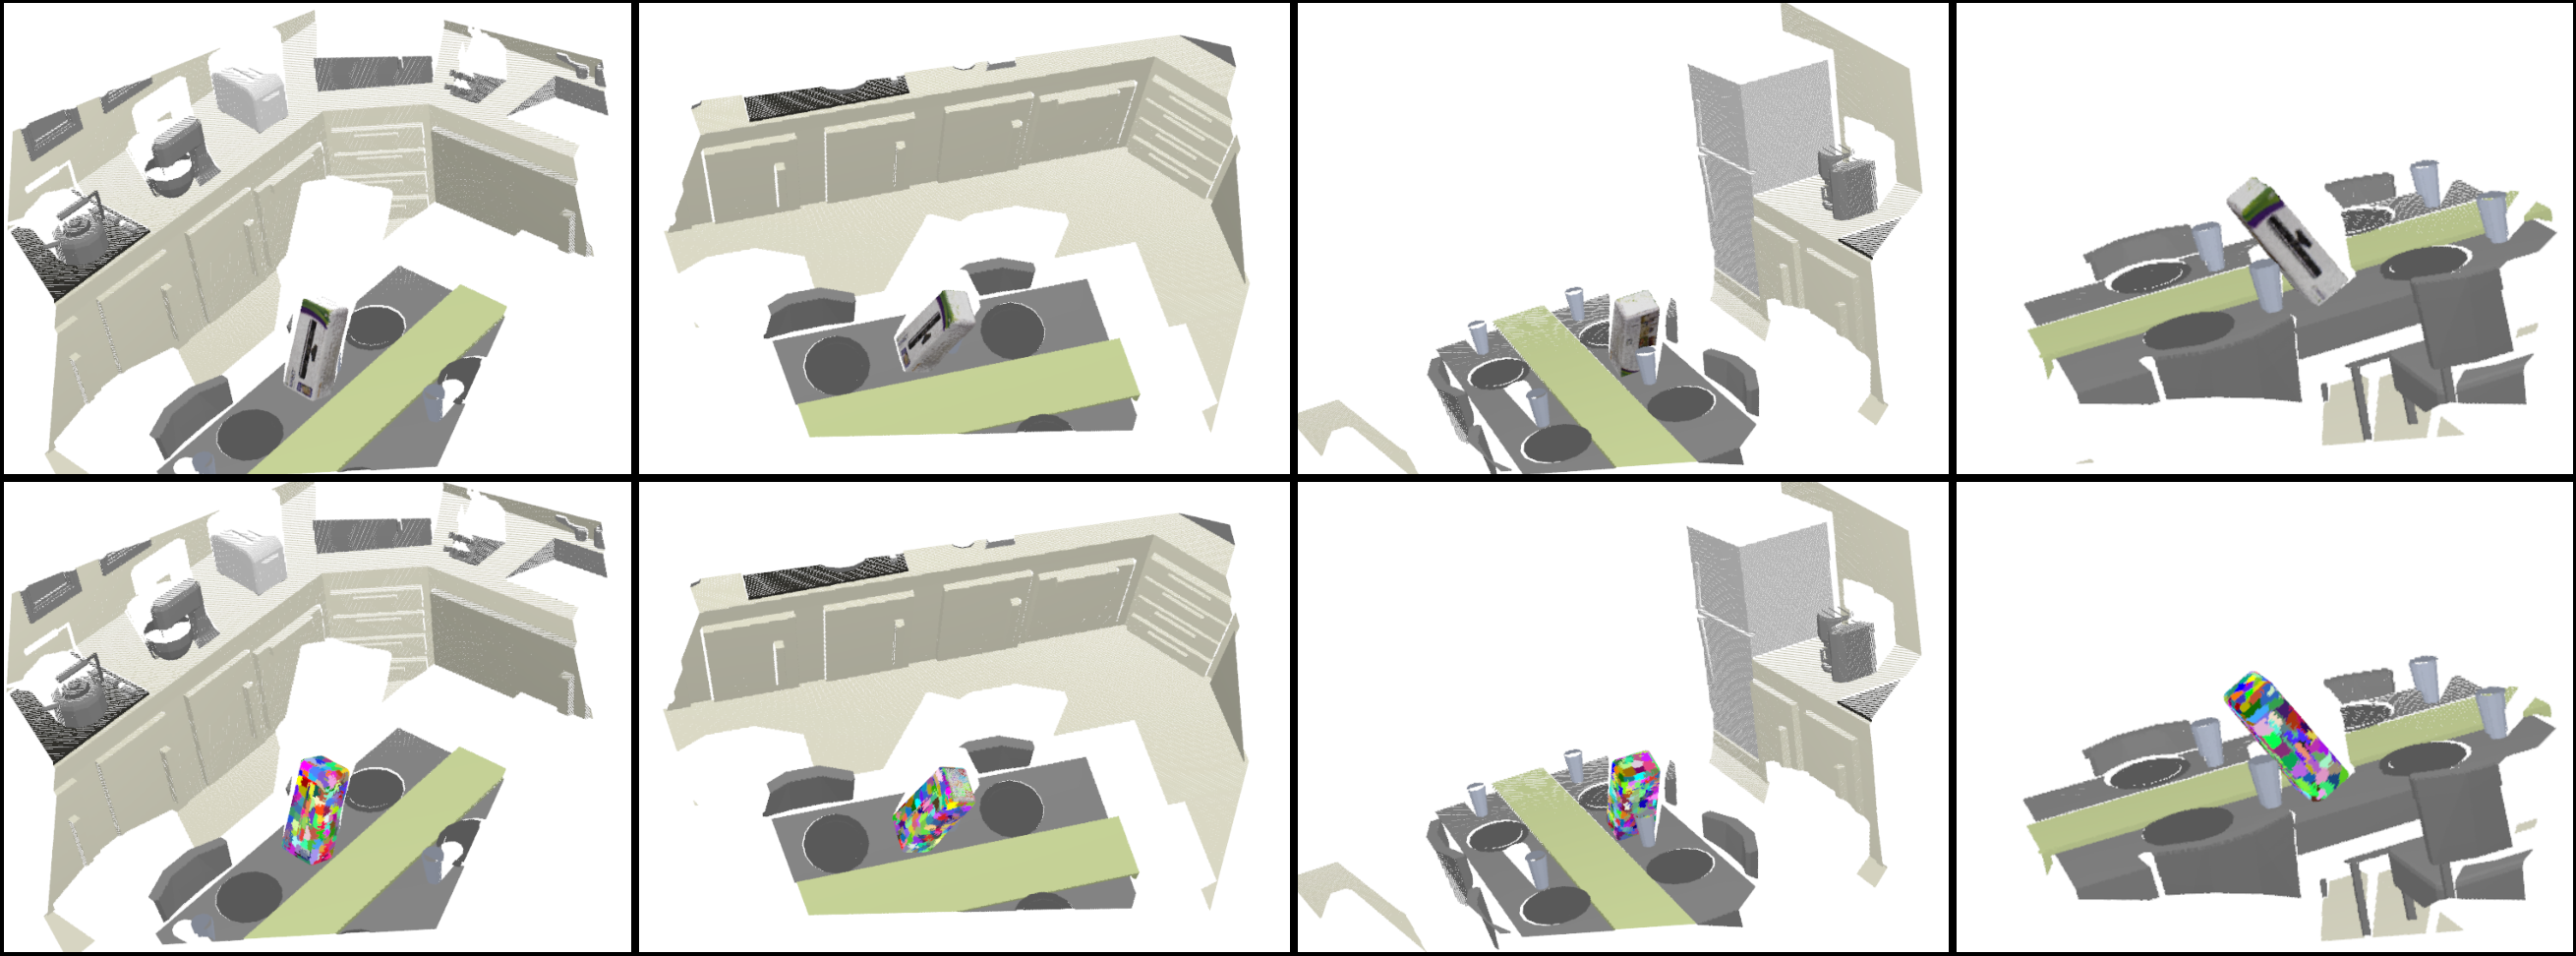
\includegraphics[width=\linewidth]{figures/Tracking/KinectBoxSVMontage.pdf}
  \caption[Tracking on the artificial ``Kinect Box'' sequence.]{Tracking on the artificial ``Kinect Box'' sequence. The top row shows tracked output overlaid on input data, while the bottom row shows the supervoxel strata that are used for sampling.}
  \label{fig:KinectBoxMontage}
\end{figure}

\section{Experimental Results}
\label{sec:ExperimentalResults}
In this Section we first present results on a set of synthetic videos to quantify the effect of the stratified sampling, and compare results to a state of the art GPU particle filter \cite{Choi_IROS2013}. We then present qualitative results on real videos in a robotic learning application, where we track multiple interacting targets with significant occlusions. In both synthetic and real cases, input consists of RGB-D sequences. Trackers were initialized using an external pose - in the synthetic case, from ground truth, and in the real case, using a pose estimation algorithm \cite{Buch_CVPR2014}. Object models were generated by registering multiple views of the objects using the same RGB-D sensor employed for tracking. All experiments were performed on a standard desktop computer (Intel i7 3.2Ghz), using all four available cores.

\subsection{Results on Synthetic Sequences}
In our first experiment, we demonstrate the effectiveness of our stratified sampling strategy using four synthetic tracking videos from \cite{Choi_IROS2013}. These RGB-D sequences are set in a virtual kitchen (see Figure \ref{fig:KinectBoxMontage}) and each contain a single item to track as the camera moves. Ground truth trajectories of the cameras are given in Figures \ref{fig:PlotsKinectBox}-\ref{fig:PlotsTide}; one can observe that the trajectories are complex, consisting of large variations in position, orientation, and velocity.  

\begin{figure}[!t]
  \centering
  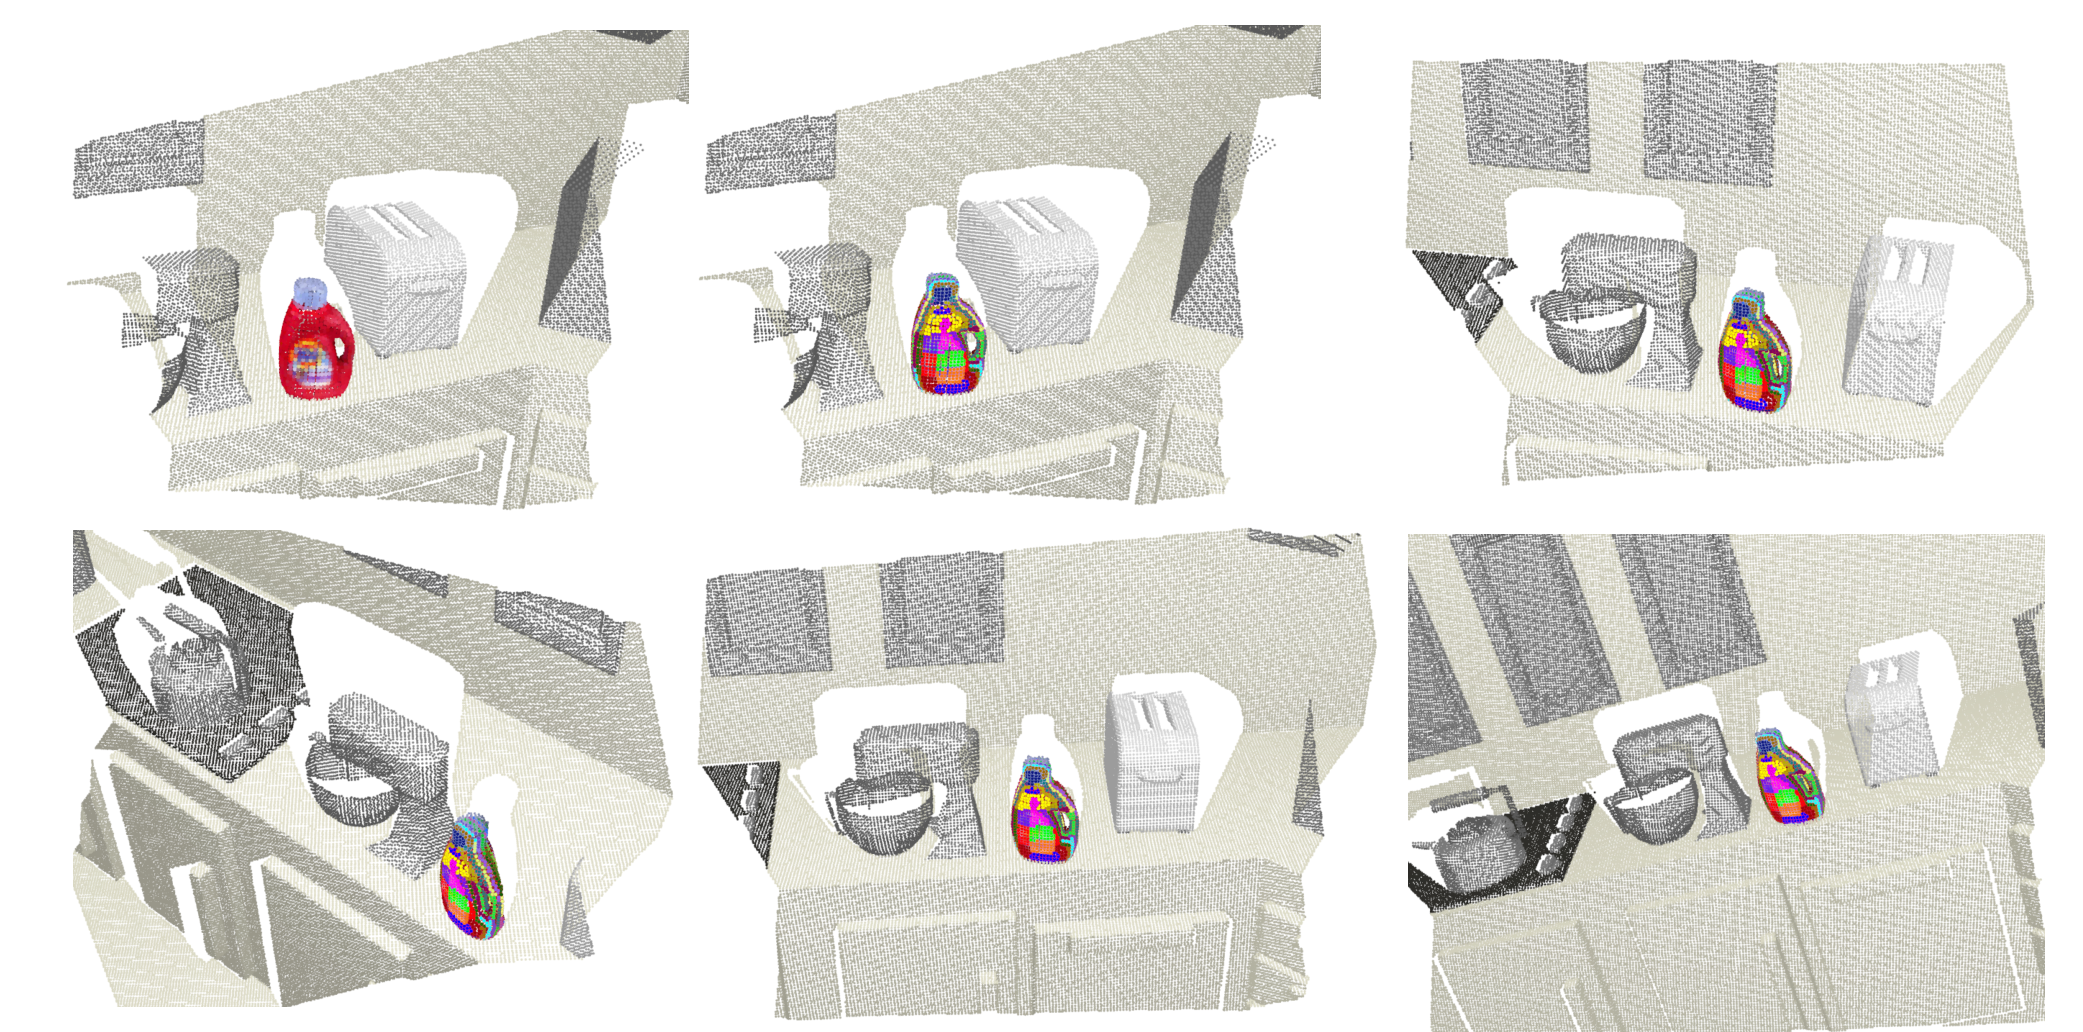
\includegraphics[width=1.06\linewidth]{figures/Tracking/TideMontage.pdf}
  \caption[Tracking on the artificial ``Tide'' sequence.]{Tracking on the artificial ``Tide'' sequence. The left column shows tracked output overlaid on input data, while the right column shows the supervoxel strata that are used for sampling.}
  \label{fig:TideMontage}
\end{figure}


To evaluate our approach, we compute root mean square (RMS) error in both translation and orientation, averaged over 25 test runs for each sequence. Computation times are measured in ms per frame, and are also averaged across all frames of the 25 test runs. In order to compare with \cite{Choi_IROS2013}, we have combined their RMS error results for each dimension (x, y, z, roll, pitch, yaw) into two measurements - displacement and rotation. Rotation is calculated using the unit quaternion distance metric \cite{Kuffner_ICRA2004}, which is equivalent to the angular distance on the unit sphere. This combination reduces the amount of data to compare without loss, as the choice of orientation of the dimensions is arbitrary and without import. Example displacement and rotation ground truths for the ``Kinect Box'' sequence can be found in Figure \ref{fig:Plots}.

Timing results are given in Figures \ref{fig:ErrorPlotsKinectBox} -\ref{fig:ErrorPlotsTide}, showing results for the four sequences, with each plot scanning across number of particles and number of sample points. Results for all four sequences are similar. One can observe that, for a given level of sampling, the RMS error decreases for both displacement and rotation as the number of particles increases. More importantly, it is also apparent that, for a given level of error, run-time per frame can be minimized by reducing the number of samples used and increasing the number of particles. Additionally, one can observe that RMS error appears to be asymptotic, with lower sampling levels approaching the asymptote at lower run-times.

We should also note that the minimum error asymptote observed is likely a consequence of the sampling resolution of the synthetic Kinect camera. For example, in the ``Kinect Box'' sequence, average distance to neighboring points (8-neighborhood) on the tracked box surface is 3.3 mm. This corresponds almost exactly to our observed error asymptote. This can be observed in all four sequences - our minimal error corresponds closely to the average point to point resolution of the observations on the model. 



%Before we present results on real data, we shall first quantify tracker performance using \gls{vr} data. \gls{vr} data is primarily useful because it allows us to easily obtain accurate ground-truth data for object tracks and poses - something that is generally not possible with real data \cite{Rossmann2012d}. With this in mind we have developed a \gls{vr} setup and benchmark \cite{VR_Benchmark_Paper} which simulates the platform we shall use in the real data shown later. The virtual platform has many simulated cameras, but in these tests we use two simulated Kinect RGB-D sensors with overlapping fields of view covering the entire work area. The sensor simulation can generate benchmark images and point clouds with controlled levels of quality, from ``ideal'' to ``real''. \footnote{Here, ``real'' is defined by the similarity of outcomes when real and simulated data are processed by libraries such as OpenCV and PCL, e.g. color histograms (RGB deviation, RGB saturation), edge detection, SURF feature detection and RANSAC feature similarity.} In the following tests we used the standard depth error of the Kinect as our lowest noise level and compared the algorithms with less accurate testdata.

%Once again, our benchmarking task is assembly of the well-established ``Cranfield'' set \cite{Collins1985,Schou2012,Martinez2014} (see Fig. \ref{fig:cad_models}).The actual assembly actions in \gls{vr} are carried out and tracked with a data-glove, generating accurate, objective ground-truth data, e.g. exact object positions as well as detailed information on the timing and existence of object manipulations and spatial relations between manipulated objects. Comparisons of real and virtual images were made in the project FastMap \cite{Rossmann2012b} and showed that artificial and real images led to very similar result in computer vision algorithms. 

%In our first experiment, we demonstrate the effectiveness of our stratified sampling strategy. We used a simple scenario in which we must track two bolts as they are picked up and inserted into a faceplate. To simplify the analysis, we fix the run-time variable by setting a desired frame-rate of 20fps \footnote{All these experiments were run on the same machine - an i7 980x with 32g of memory}, and then determined experimentally the number of particles for which this frame rate was sustainable at different degrees of sampling. Degree of sampling is simply the ratio of the number of points sampled to the number of points present in the model, $\frac{N_s}{N_m}$. Table \ref{table:timing} gives the average frame rates and standard deviation measured during the runs. Figure \ref{TODOFIGURE} shows average error rates for the different degrees of sampling. Additionally, Figure \ref{TODOFIGURE} shows the affect on error and run time of increased particle number for fixed degrees of sampling. Finally, Figure \ref{fig:CombinedNoNoise} gives an example of what the tracked output looks like versus ground truth - it is evident that the tracker is able to follow the objects quite well in terms of translation. Rotations, on the other hand, are much noisier, due to the rotational symmetries present in the tracked object (the bolt).  

%%%%%%%%%%%%%%%%%%%%%%%%%%%%%%%%%%%%%%%%%%%%%%%%%%%%%%%%%%
\begin{figure*}[!ht]
  \centering
  \subfloat{{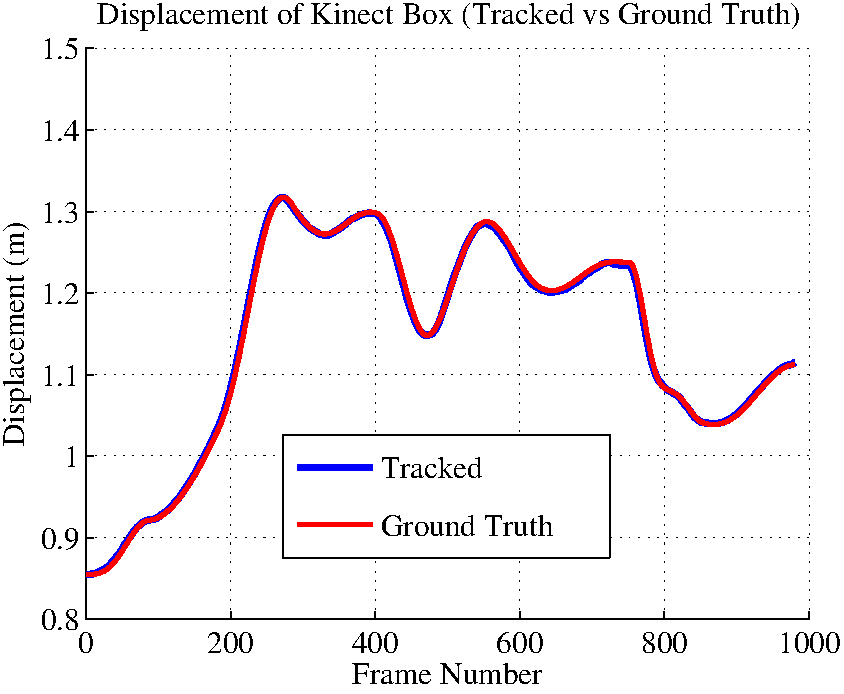
\includegraphics[width=.46\textwidth]{figures/Tracking/ErrorComps/DispKinectBox.pdf} }} %
  \qquad
  \subfloat{{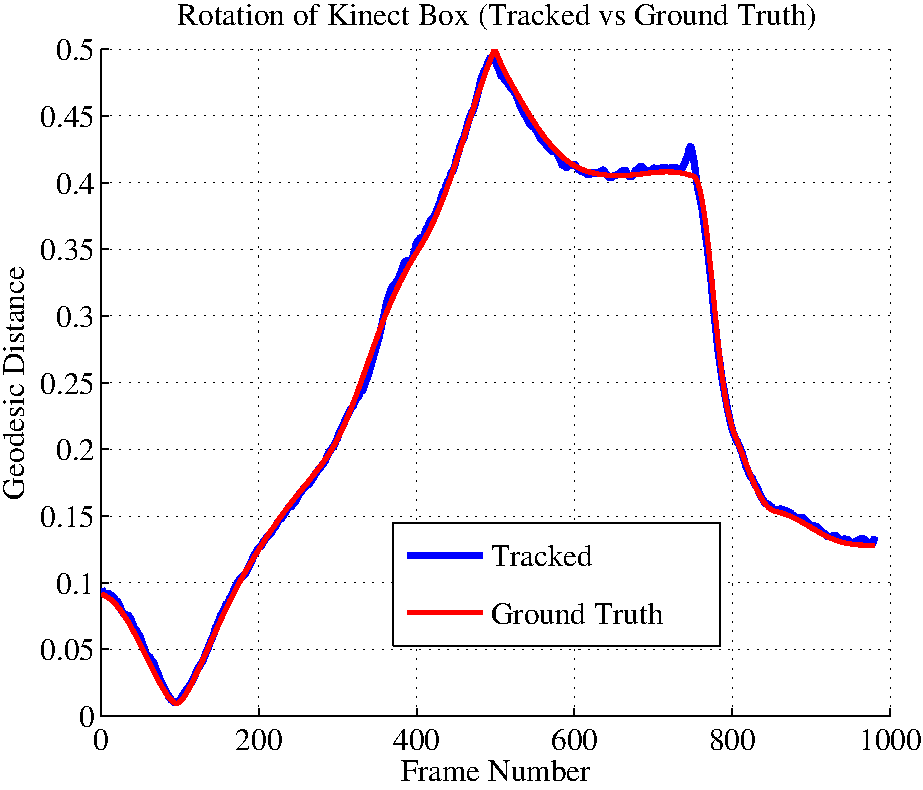
\includegraphics[width=.46\textwidth]{figures/Tracking/ErrorComps/AngleKinectBox.pdf} }}%
  \caption[Tracked vs Ground Truth - Kinect Box]{Displacement and rotation ground truth, with an example tracked result from a single run at $N_{samples}=100$ and $N_{particles}=1000$ (a frame rate of 20 fps).}%
  \label{fig:PlotsKinectBox}%
\end{figure*}

\begin{figure*}[!ht]
  \centering 
  \vspace{-10pt}
  \subfloat{{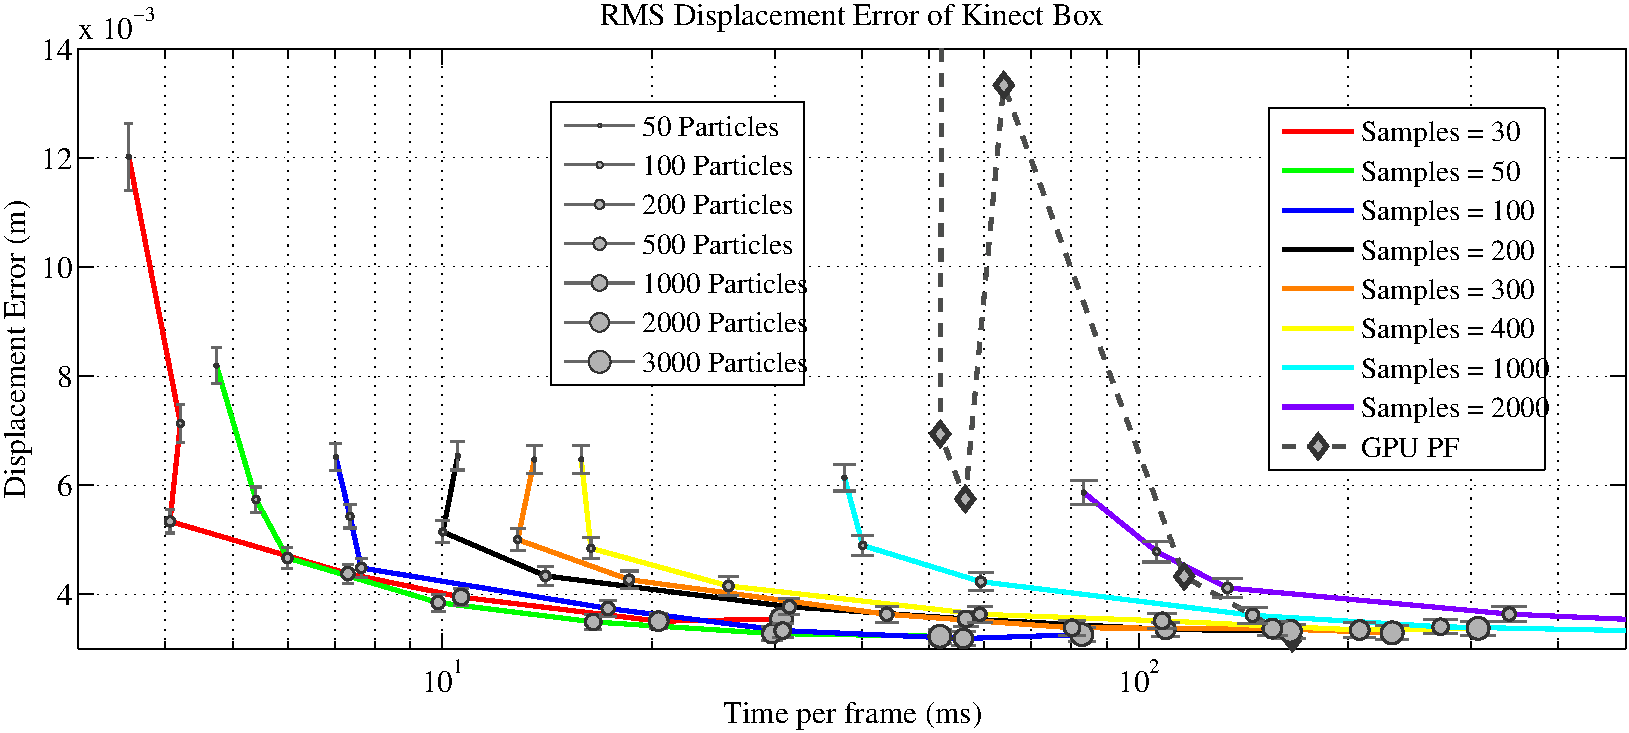
\includegraphics[width=1.0\linewidth]{figures/Tracking/ErrorComps/DispErrorKinectBox.pdf} }} \\
  \vspace{-10pt}
  \subfloat{{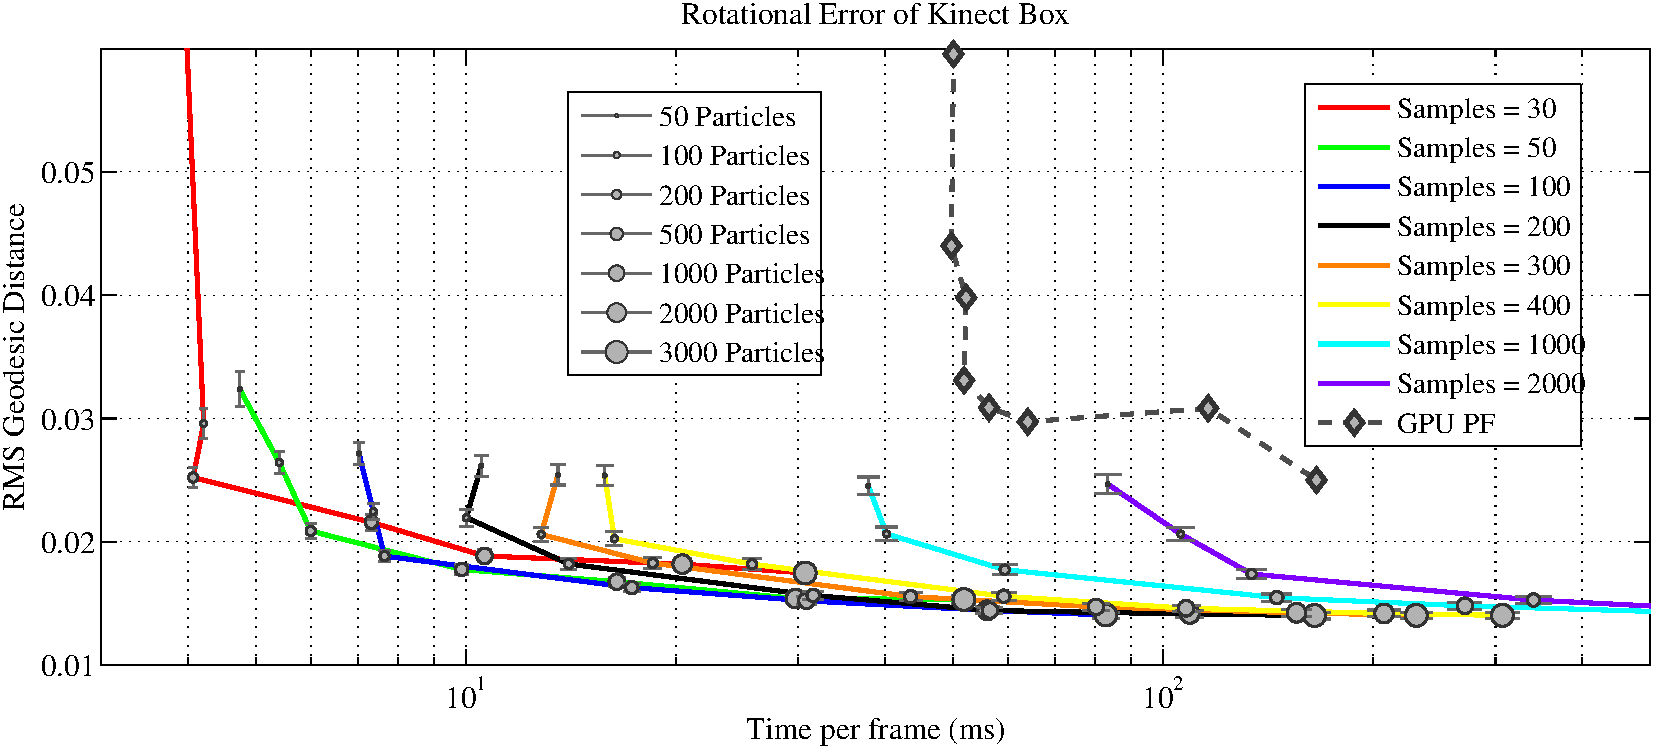
\includegraphics[width=1.0\linewidth]{figures/Tracking/ErrorComps/AngularErrorKinectBox.pdf} }}   \vspace{-7pt} \\
  \caption[Results on the Kinect Box artificial sequence.]{Results on the Kinect Box artificial sequence. Each colored curve represents a certain number of samples, and gives mean RMS error averaged over 25 trial runs for increasing numbers of particles.}%
  \label{fig:ErrorPlotsKinectBox}%
\end{figure*}
%%%%%%%%%%%%%%%%%%%%%%%%%%%%%%%%%%%%%%%%%%%%%%%%%%%%%%%%%%
\begin{figure*}[!ht]
  \centering
  \subfloat{{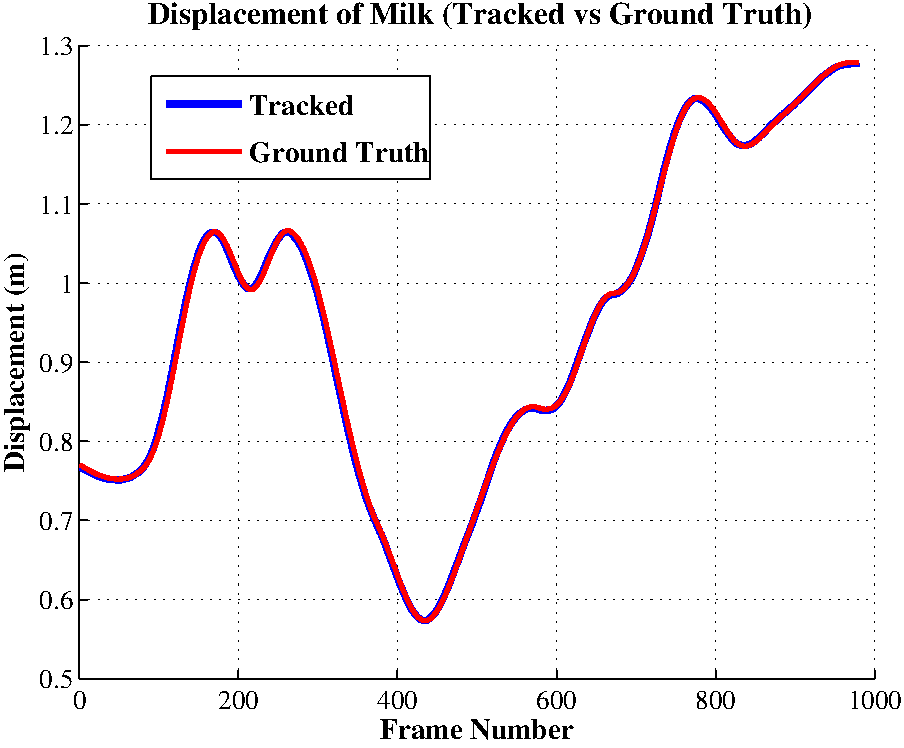
\includegraphics[width=.46\textwidth]{figures/Tracking/ErrorComps/DispMilk.pdf} }} %
  \qquad
  \subfloat{{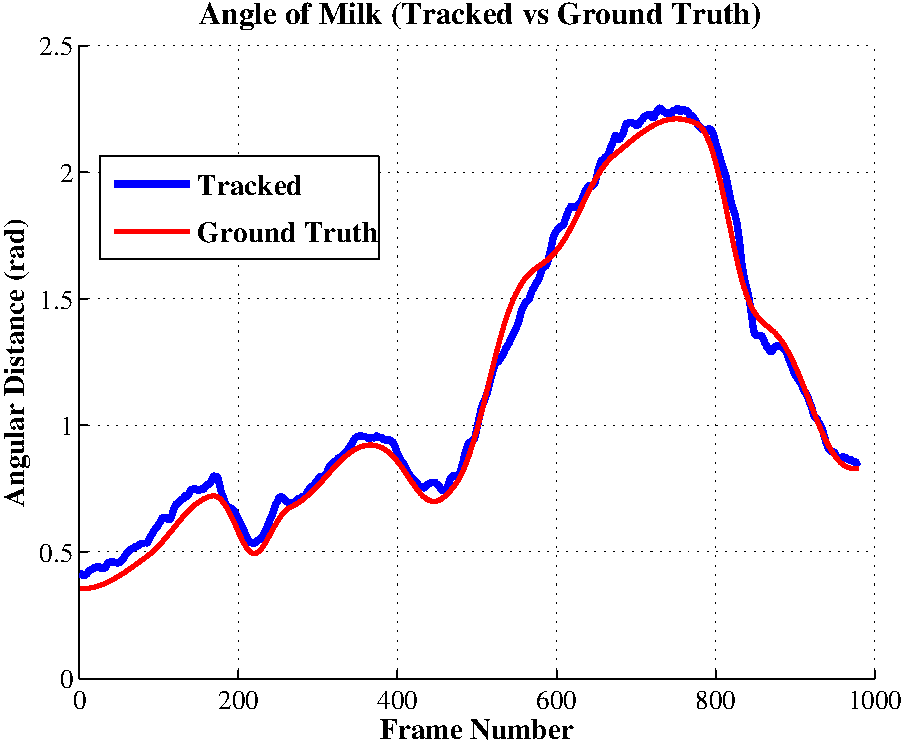
\includegraphics[width=.46\textwidth]{figures/Tracking/ErrorComps/AngleMilk.pdf} }}%
  \caption[Tracked vs Ground Truth - Milk]{Displacement and rotation ground truth, with an example tracked result from a single run at $N_{samples}=100$ and $N_{particles}=1000$ (a frame rate of 20 fps).}%
  \label{fig:PlotsMilk}%
\end{figure*}

\begin{figure*}[!ht]
  \centering 
  \vspace{-10pt}
  \subfloat{{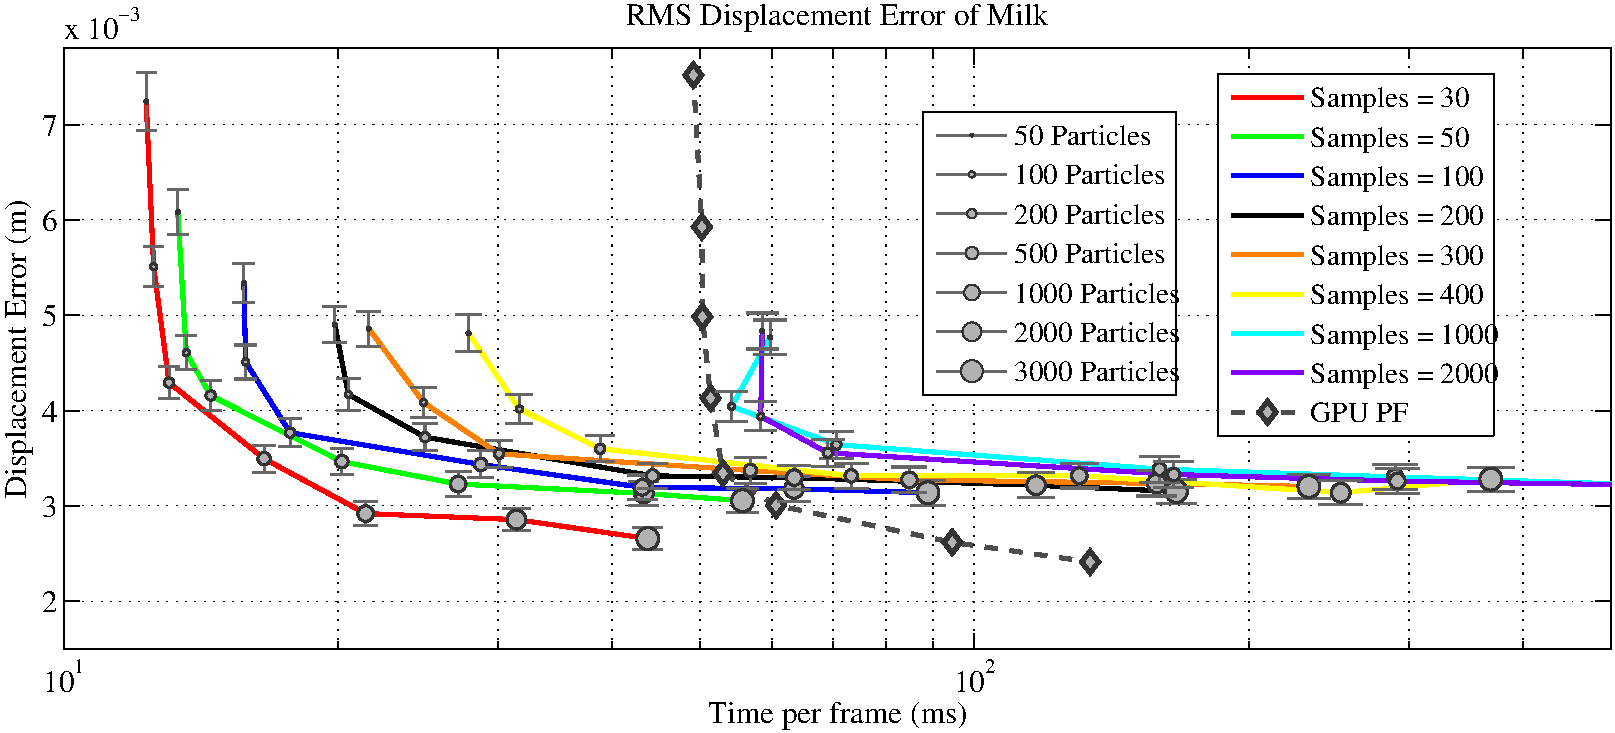
\includegraphics[width=0.98\linewidth]{figures/Tracking/ErrorComps/DispErrorMilk.pdf} }} \\
  \vspace{-10pt}
  \subfloat{{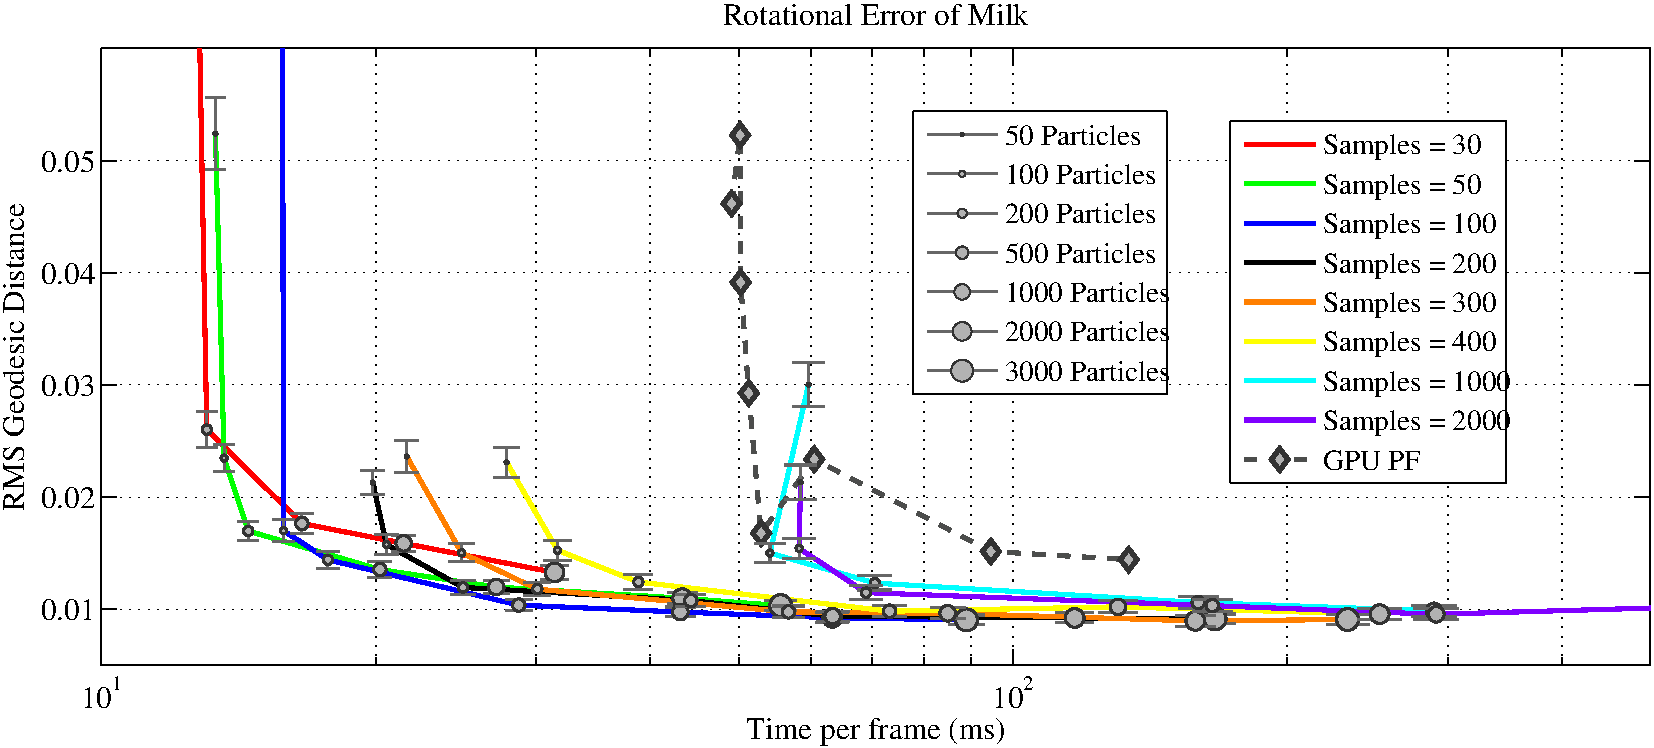
\includegraphics[width=1.0\linewidth]{figures/Tracking/ErrorComps/AngularErrorMilk.pdf} }}   \vspace{-7pt} \\
  \caption[Results on the Milk artificial sequence.]{Results on the Milk artificial sequence. Each colored curve represents a certain number of samples, and gives mean RMS error averaged over 25 trial runs for increasing numbers of particles.}%
  \label{fig:ErrorPlotsMilk}%
\end{figure*}
%%%%%%%%%%%%%%%%%%%%%%%%%%%%%%%%%%%%%%%%%%%%%%%%%%%%%%%%%%
\begin{figure*}[!ht]
  \centering
  \subfloat{{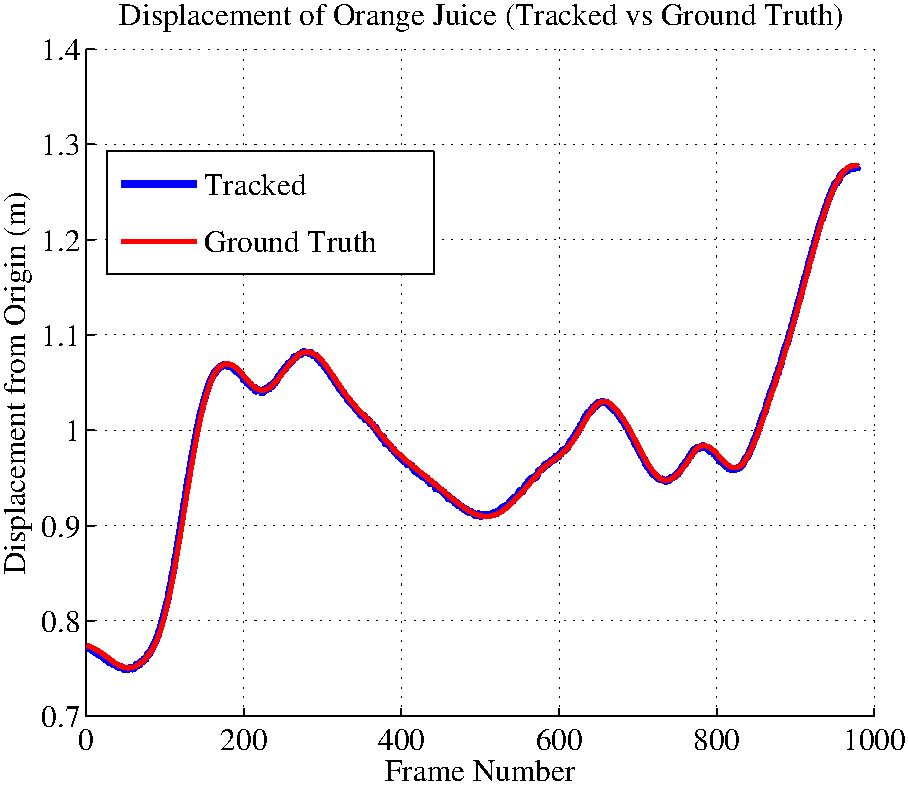
\includegraphics[width=.46\textwidth]{figures/Tracking/ErrorComps/DispOrangeJuice.pdf} }} %
  \qquad
  \subfloat{{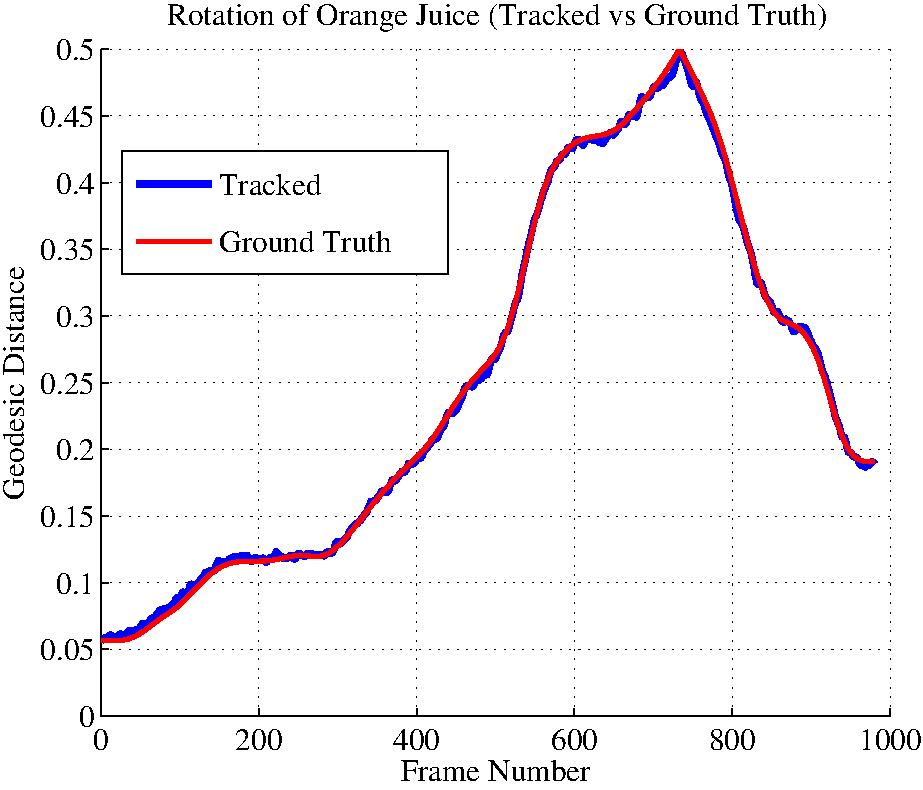
\includegraphics[width=.46\textwidth]{figures/Tracking/ErrorComps/AngleOrangeJuice.pdf} }}%
  \caption[Tracked vs Ground Truth - Orange Juice]{Displacement and rotation ground truth, with an example tracked result from a single run at $N_{samples}=100$ and $N_{particles}=1000$ (a frame rate of 20 fps).}%
  \label{fig:PlotsOrangeJuice}%
\end{figure*}

\begin{figure*}[!ht]
  \centering 
  \vspace{-10pt}
  \subfloat{{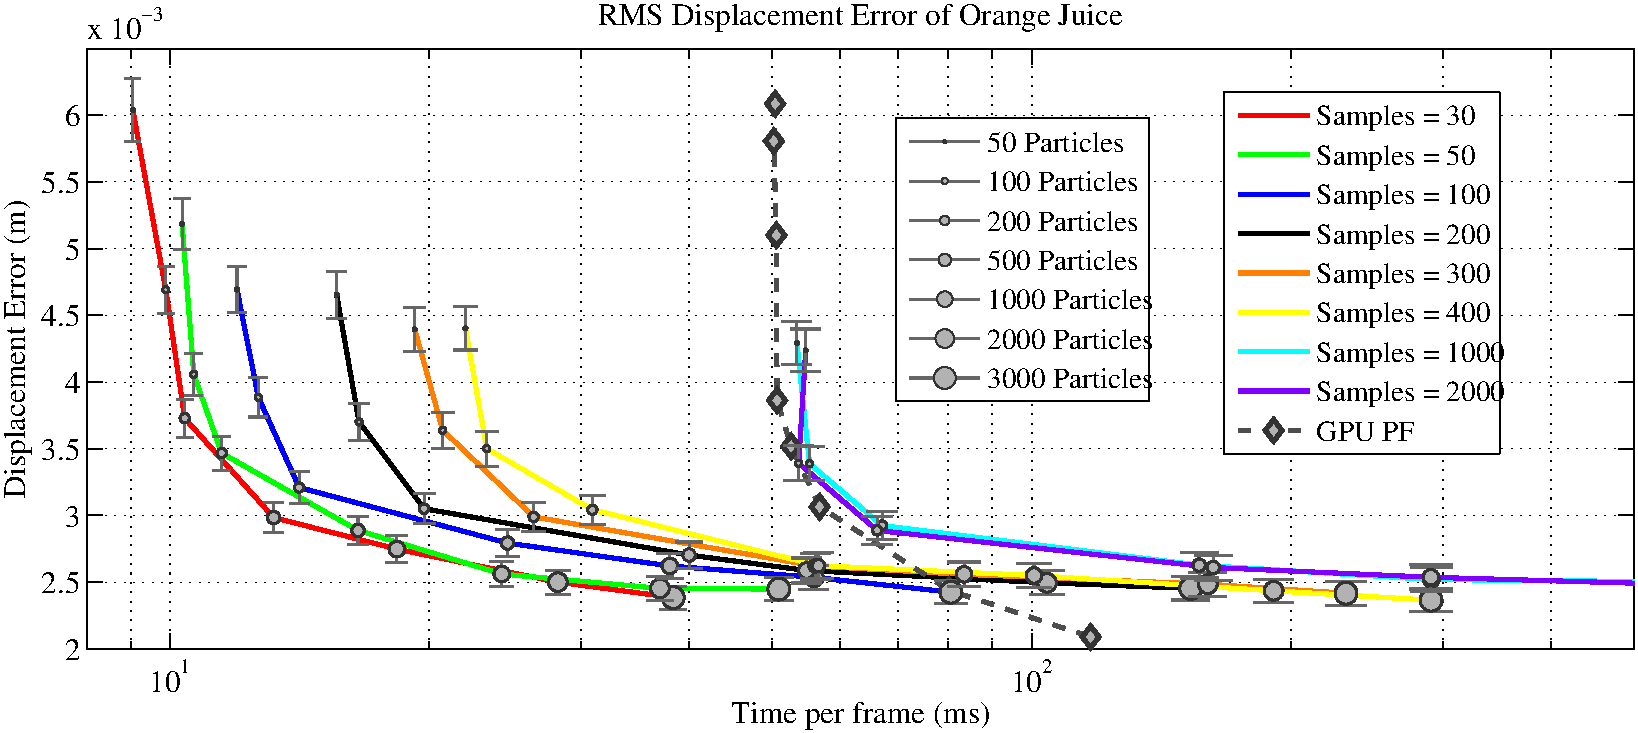
\includegraphics[width=0.98\linewidth]{figures/Tracking/ErrorComps/DispErrorOrangeJuice.pdf} }} \\
  \vspace{-10pt}
  \subfloat{{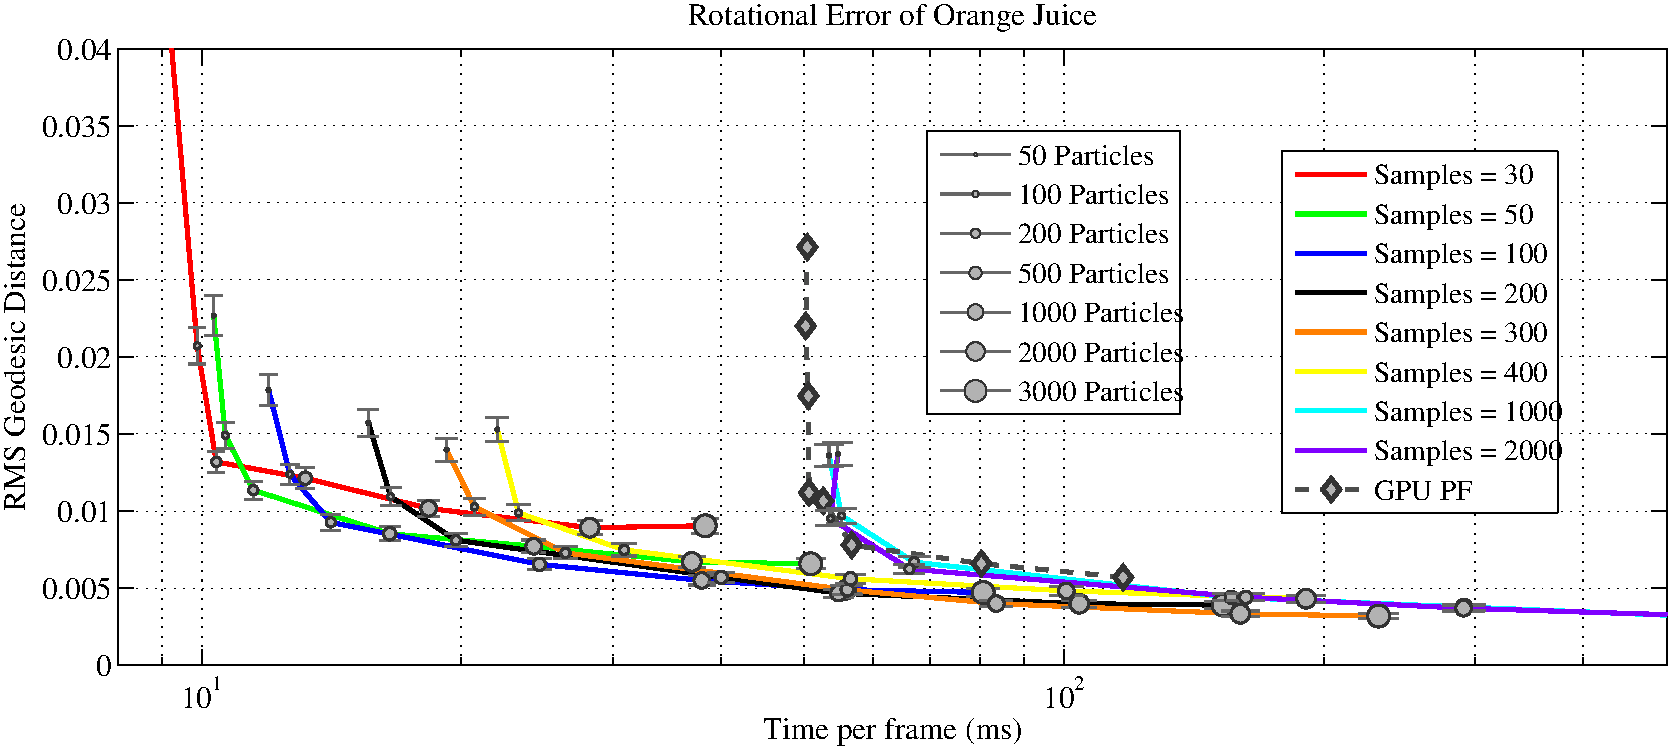
\includegraphics[width=1.0\linewidth]{figures/Tracking/ErrorComps/AngularErrorOrangeJuice.pdf} }}   \vspace{-7pt} \\
  \caption[Results on the Orange Juice artificial sequence.]{Results on the Orange Juice artificial sequence. Each colored curve represents a certain number of samples, and gives mean RMS error averaged over 25 trial runs for increasing numbers of particles.}%
  \label{fig:ErrorPlotsOrangeJuice}%
\end{figure*}
%%%%%%%%%%%%%%%%%%%%%%%%%%%%%%%%%%%%%%%%%%%%%%%%%%%%%%%%%%
\begin{figure*}[!ht]
  \centering
  \subfloat{{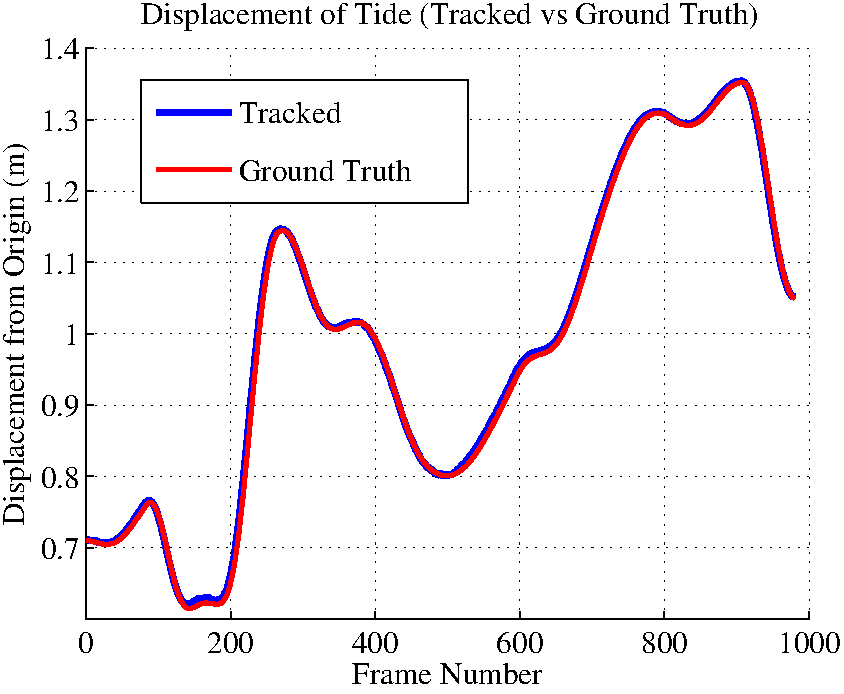
\includegraphics[width=.46\textwidth]{figures/Tracking/ErrorComps/DispTide.pdf} }} %
  \qquad
  \subfloat{{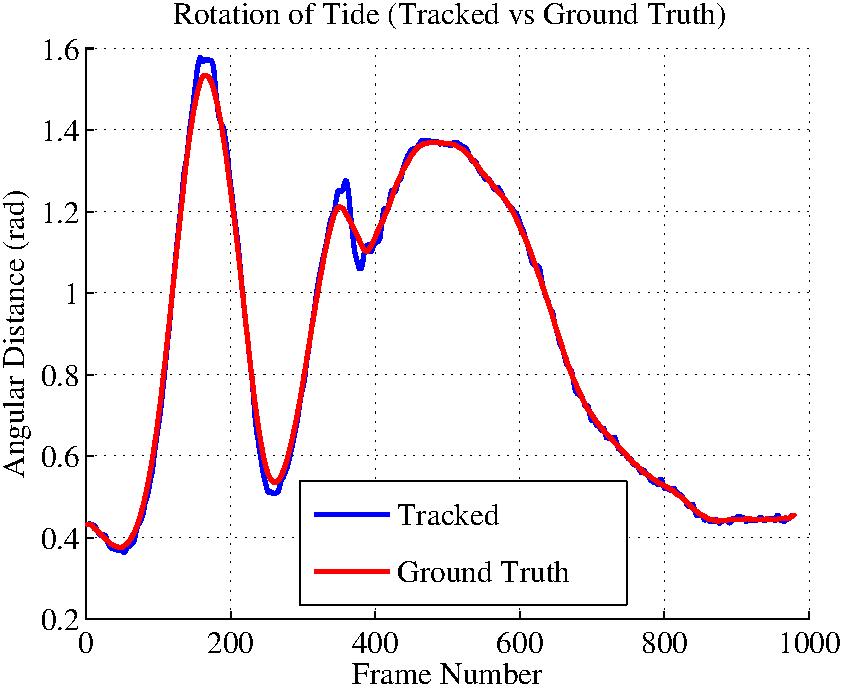
\includegraphics[width=.46\textwidth]{figures/Tracking/ErrorComps/AngleTide.pdf} }}%
  \caption[Tracked vs Ground Truth - Tide]{Displacement and rotation ground truth, with an example tracked result from a single run at $N_{samples}=100$ and $N_{particles}=1000$ (a frame rate of 20 fps).}%
  \label{fig:PlotsTide}%
\end{figure*}

\begin{figure*}[!ht]
  \centering 
  \vspace{-10pt}
  \subfloat{{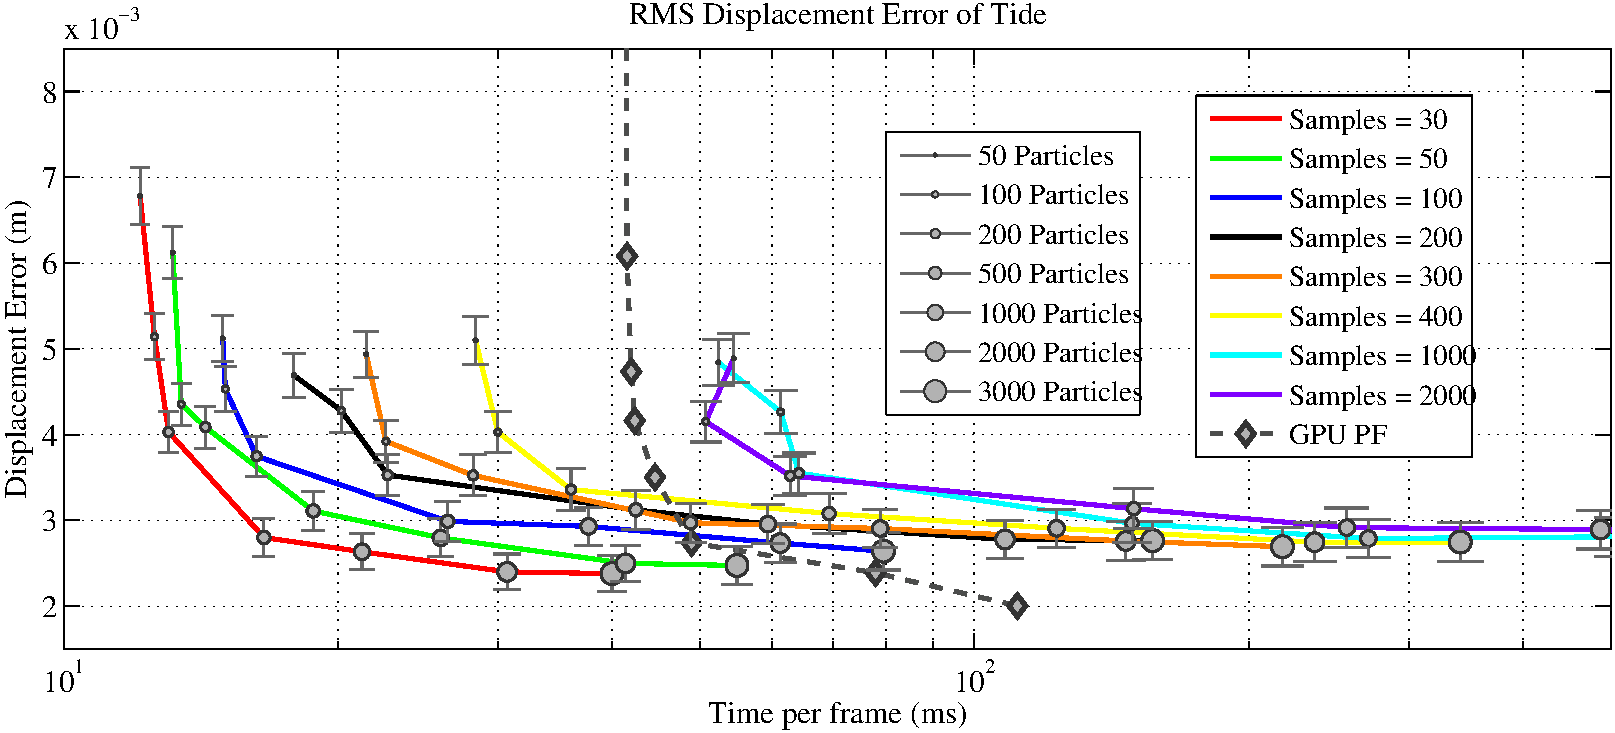
\includegraphics[width=0.98\linewidth]{figures/Tracking/ErrorComps/DispErrorTide.pdf} }} \\
  \vspace{-10pt}
  \subfloat{{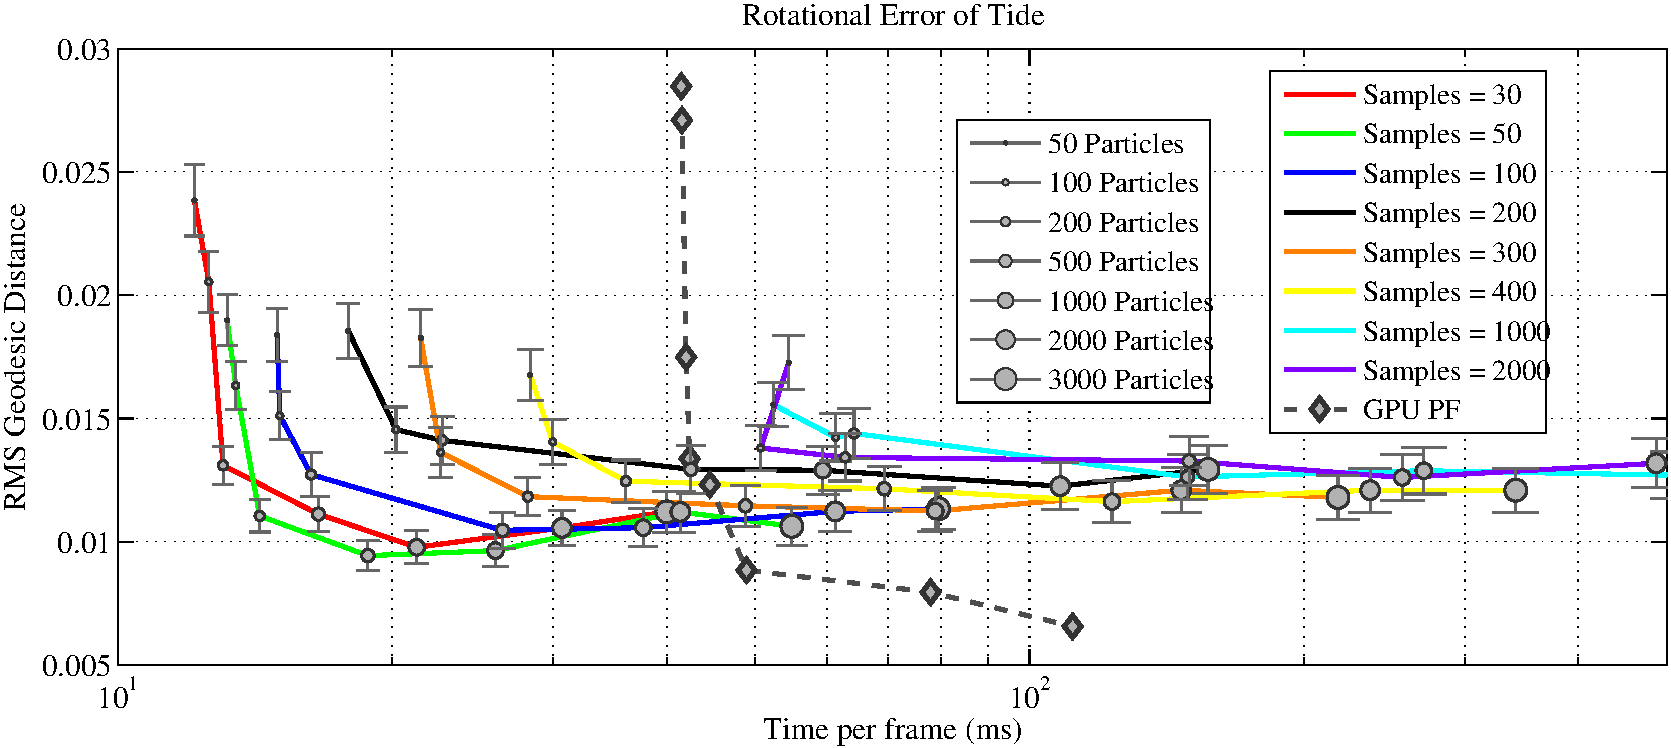
\includegraphics[width=1.0\linewidth]{figures/Tracking/ErrorComps/AngularErrorTide.pdf} }}   \vspace{-7pt} \\
  \caption[Results on the Tide artificial sequence.]{Results on the Tide artificial sequence. Each colored curve represents a certain number of samples, and gives mean RMS error averaged over 25 trial runs for increasing numbers of particles.}%
  \label{fig:ErrorPlotsTide}%
\end{figure*}
%%%%%%%%%%%%%%%%%%%%%%%%%%%%%%%%%%%%%%%%%%%%%%%%%%%%%%%%%%

Our performance compares favorably to the results of Choi and Christensen \cite{Choi_IROS2013} - for a given level of error, we achieve per-frame run times that are between half and a tenth of their published results. Additionally, we consistently reach the error asymptote at considerably lower run times. We should also note that the highest sampling level shown corresponds to a complete sampling of the model, and can be thought of as equivalent to the baseline PCL implementation, although we have made some modifications to the resampling and dynamic model which improve results. As can be seen, we are at least an order of magnitude faster than this base implementation.

\subsection{Results on Real Sequences}
One application of our tracker is to provide semantic understanding and imitation of assembly tasks. This can be accomplished by tracking all interacting parts of an assembly as a human demonstrates, and then using the trajectories and poses in order to train a robot to replicate the construction. Additionally, the tracked output can be used as an input for the robot during construction in order to verify that it has successfully completed each step of the task. 

\begin{figure*}[!ht]
  \centering
  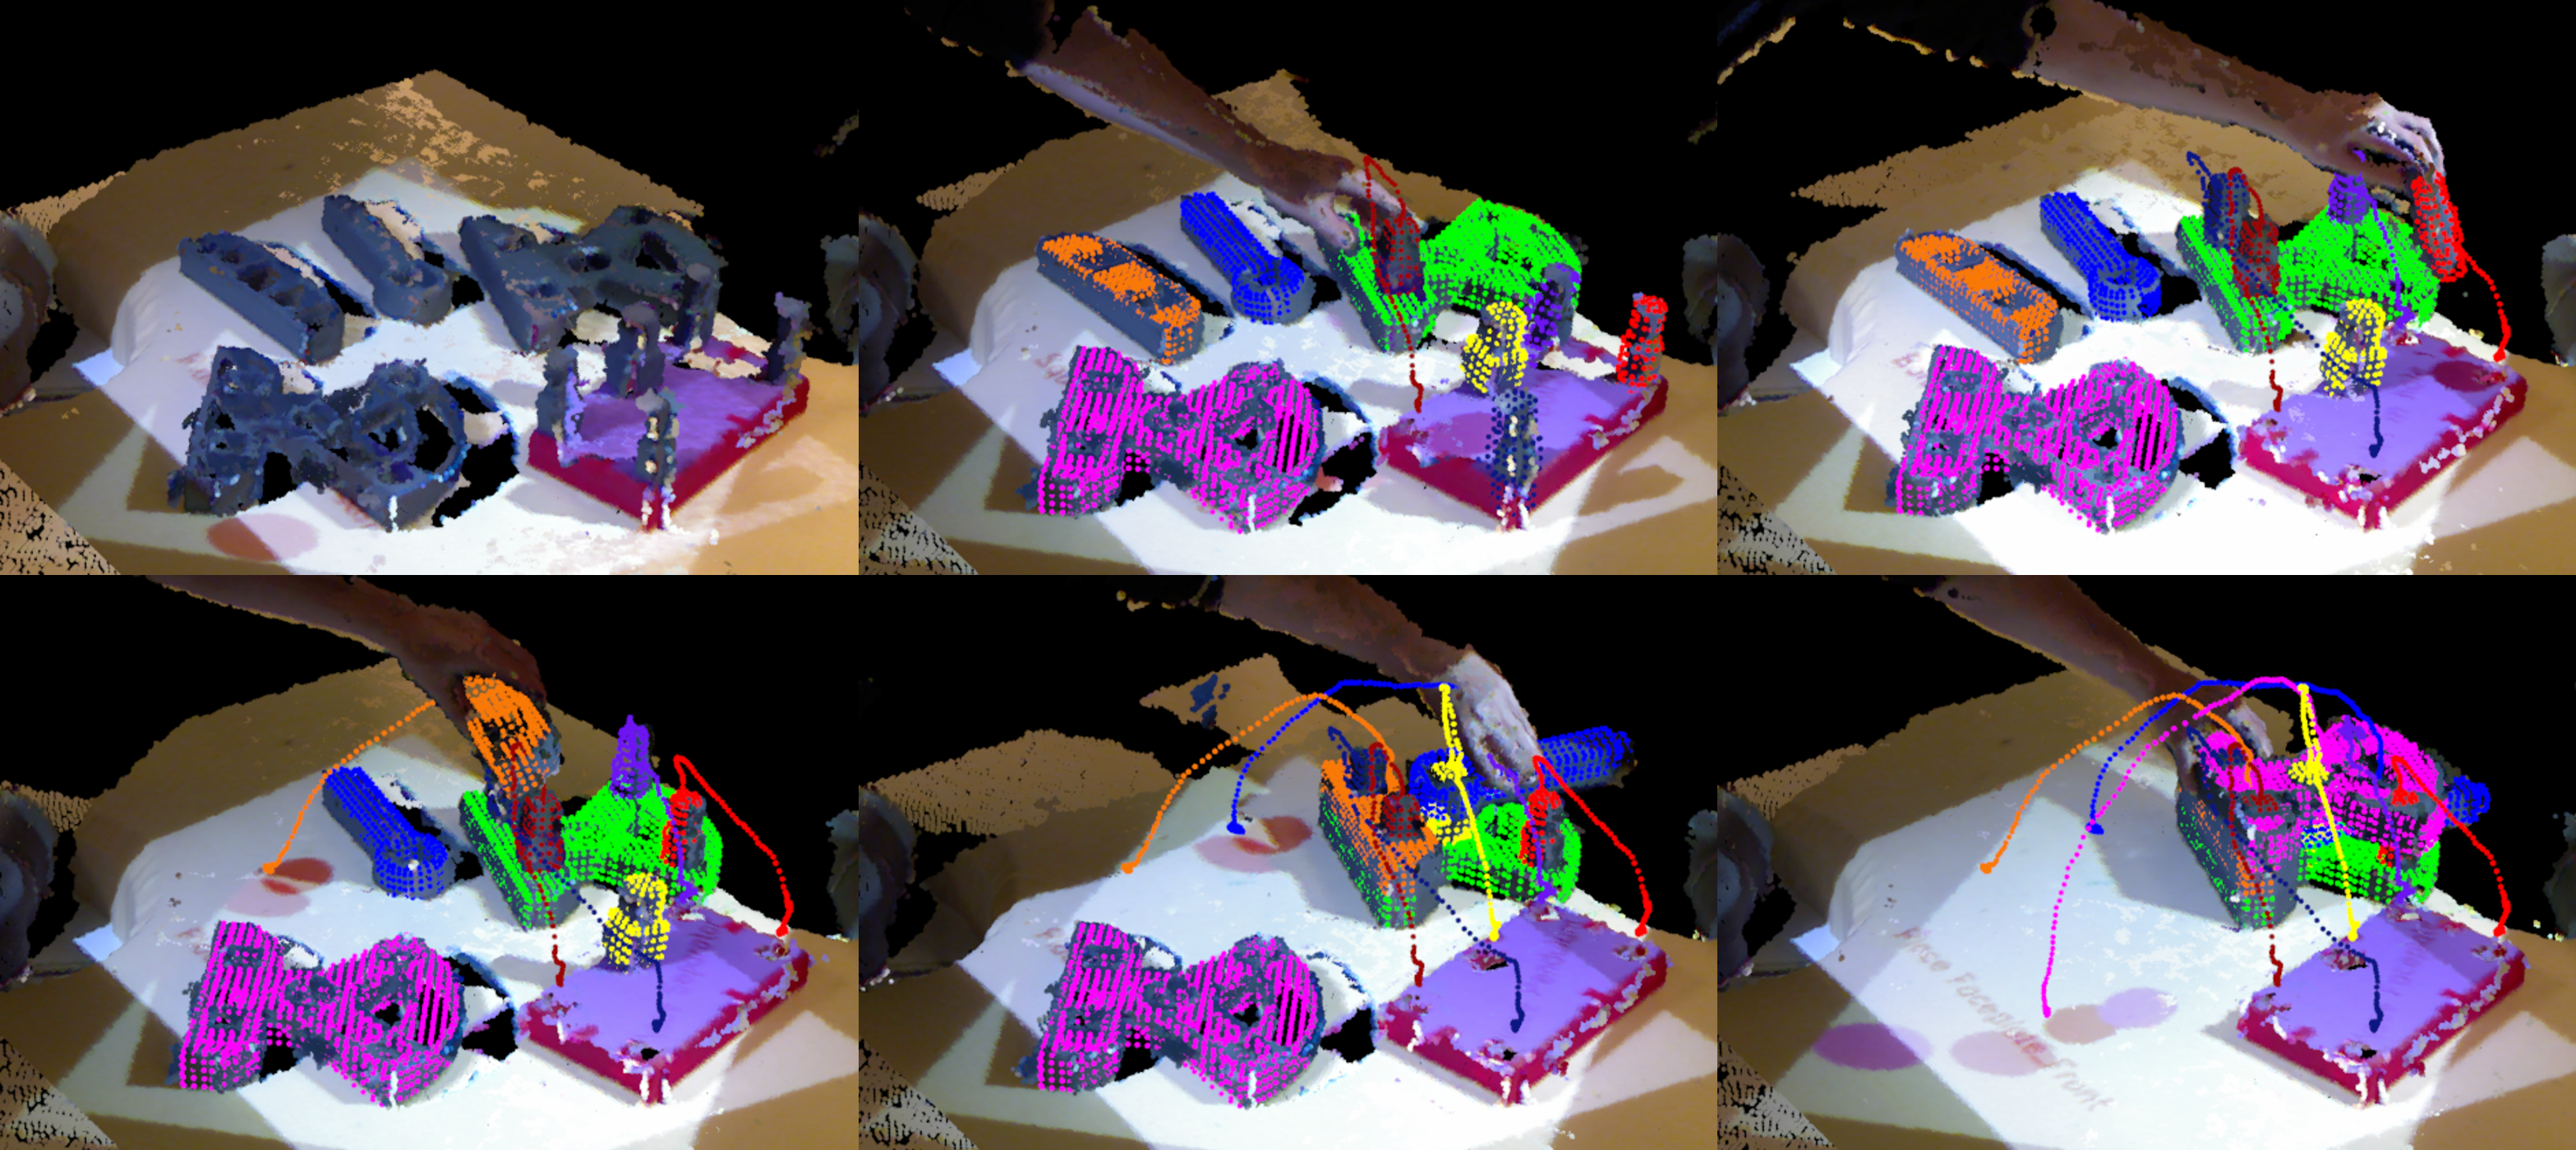
\includegraphics[width=1.0\textwidth]{figures/Tracking/HumanMontageSmall.pdf}
  \caption[Human demonstration of assembly of the Cranfield Scenario.]{Human demonstration of assembly of the Cranfield Scenario. Tracking runs live for all objects at once at sufficient frame rates to track the whole task.}
  \label{fig:Tracking_Montage}
\end{figure*}

As a demonstration of this, we shall once again use the well established ``Cranfield'' benchmark set \cite{Collins1985}, consisting of eight pieces which can be assembled in a number of different orders. In our experiments, models consist of voxelized point clouds derived from high-resolution models of the pieces, and initial poses for tracking are found using a combined object recognition and pose estimation algorithm \cite{Buch_CVPR2014}. Each object is tracked using an independent particle filter, with $N_{samples}$ set to 50, and $N_{particles}$ set to 1000. 

Recordings were made on the MARVIN platform at the University of Southern Denmark, and use 2 Kinect RGB-D cameras \footnote{It is well-known that multiple Kinect sensors sharing a common field of view will cause IR interference, resulting in poor depth reconstructions. A known solution, which the platform incorporates, is the use of vibrating motors mounted on the Kinect sensors \cite{Butler2012}. This method has been shown to effectively blur out the noisy contributions of external sensors, while maintaining a high depth reconstruction quality.}. The recordings were performed by different people, where the people were following assembly instructions presented by the planning system of the IntellAct project. A description of the planner is beyond the scope of this work (we refer the reader to \cite{Rossman_ICRA2014}), but for our purposes we just need to know that the order of assembly varies from sequence to sequence. 

Figure \ref{fig:Tracking_Montage} shows a montage of screenshots captured as a human demonstrates assembly of the benchmark. As can be seen, all pieces are successfully tracked from start to finish, with each tracker outputting smooth trajectories that can be used for training a robot using Dynamic Motion Primitives (DMP) \cite{Kulvicius2012}. In Figure \ref{fig:TrackingResults} we show tracks from multiple different human demonstrations - one can observe the different strategies that people employ in assembling the benchmark. The tracks in the lower right corner of the Figure are from a robot reproducing the assembly after being trained on the human demonstrations \cite{Rossman_ICRA2014}. 

\begin{figure*}[!ht]
  \centering
  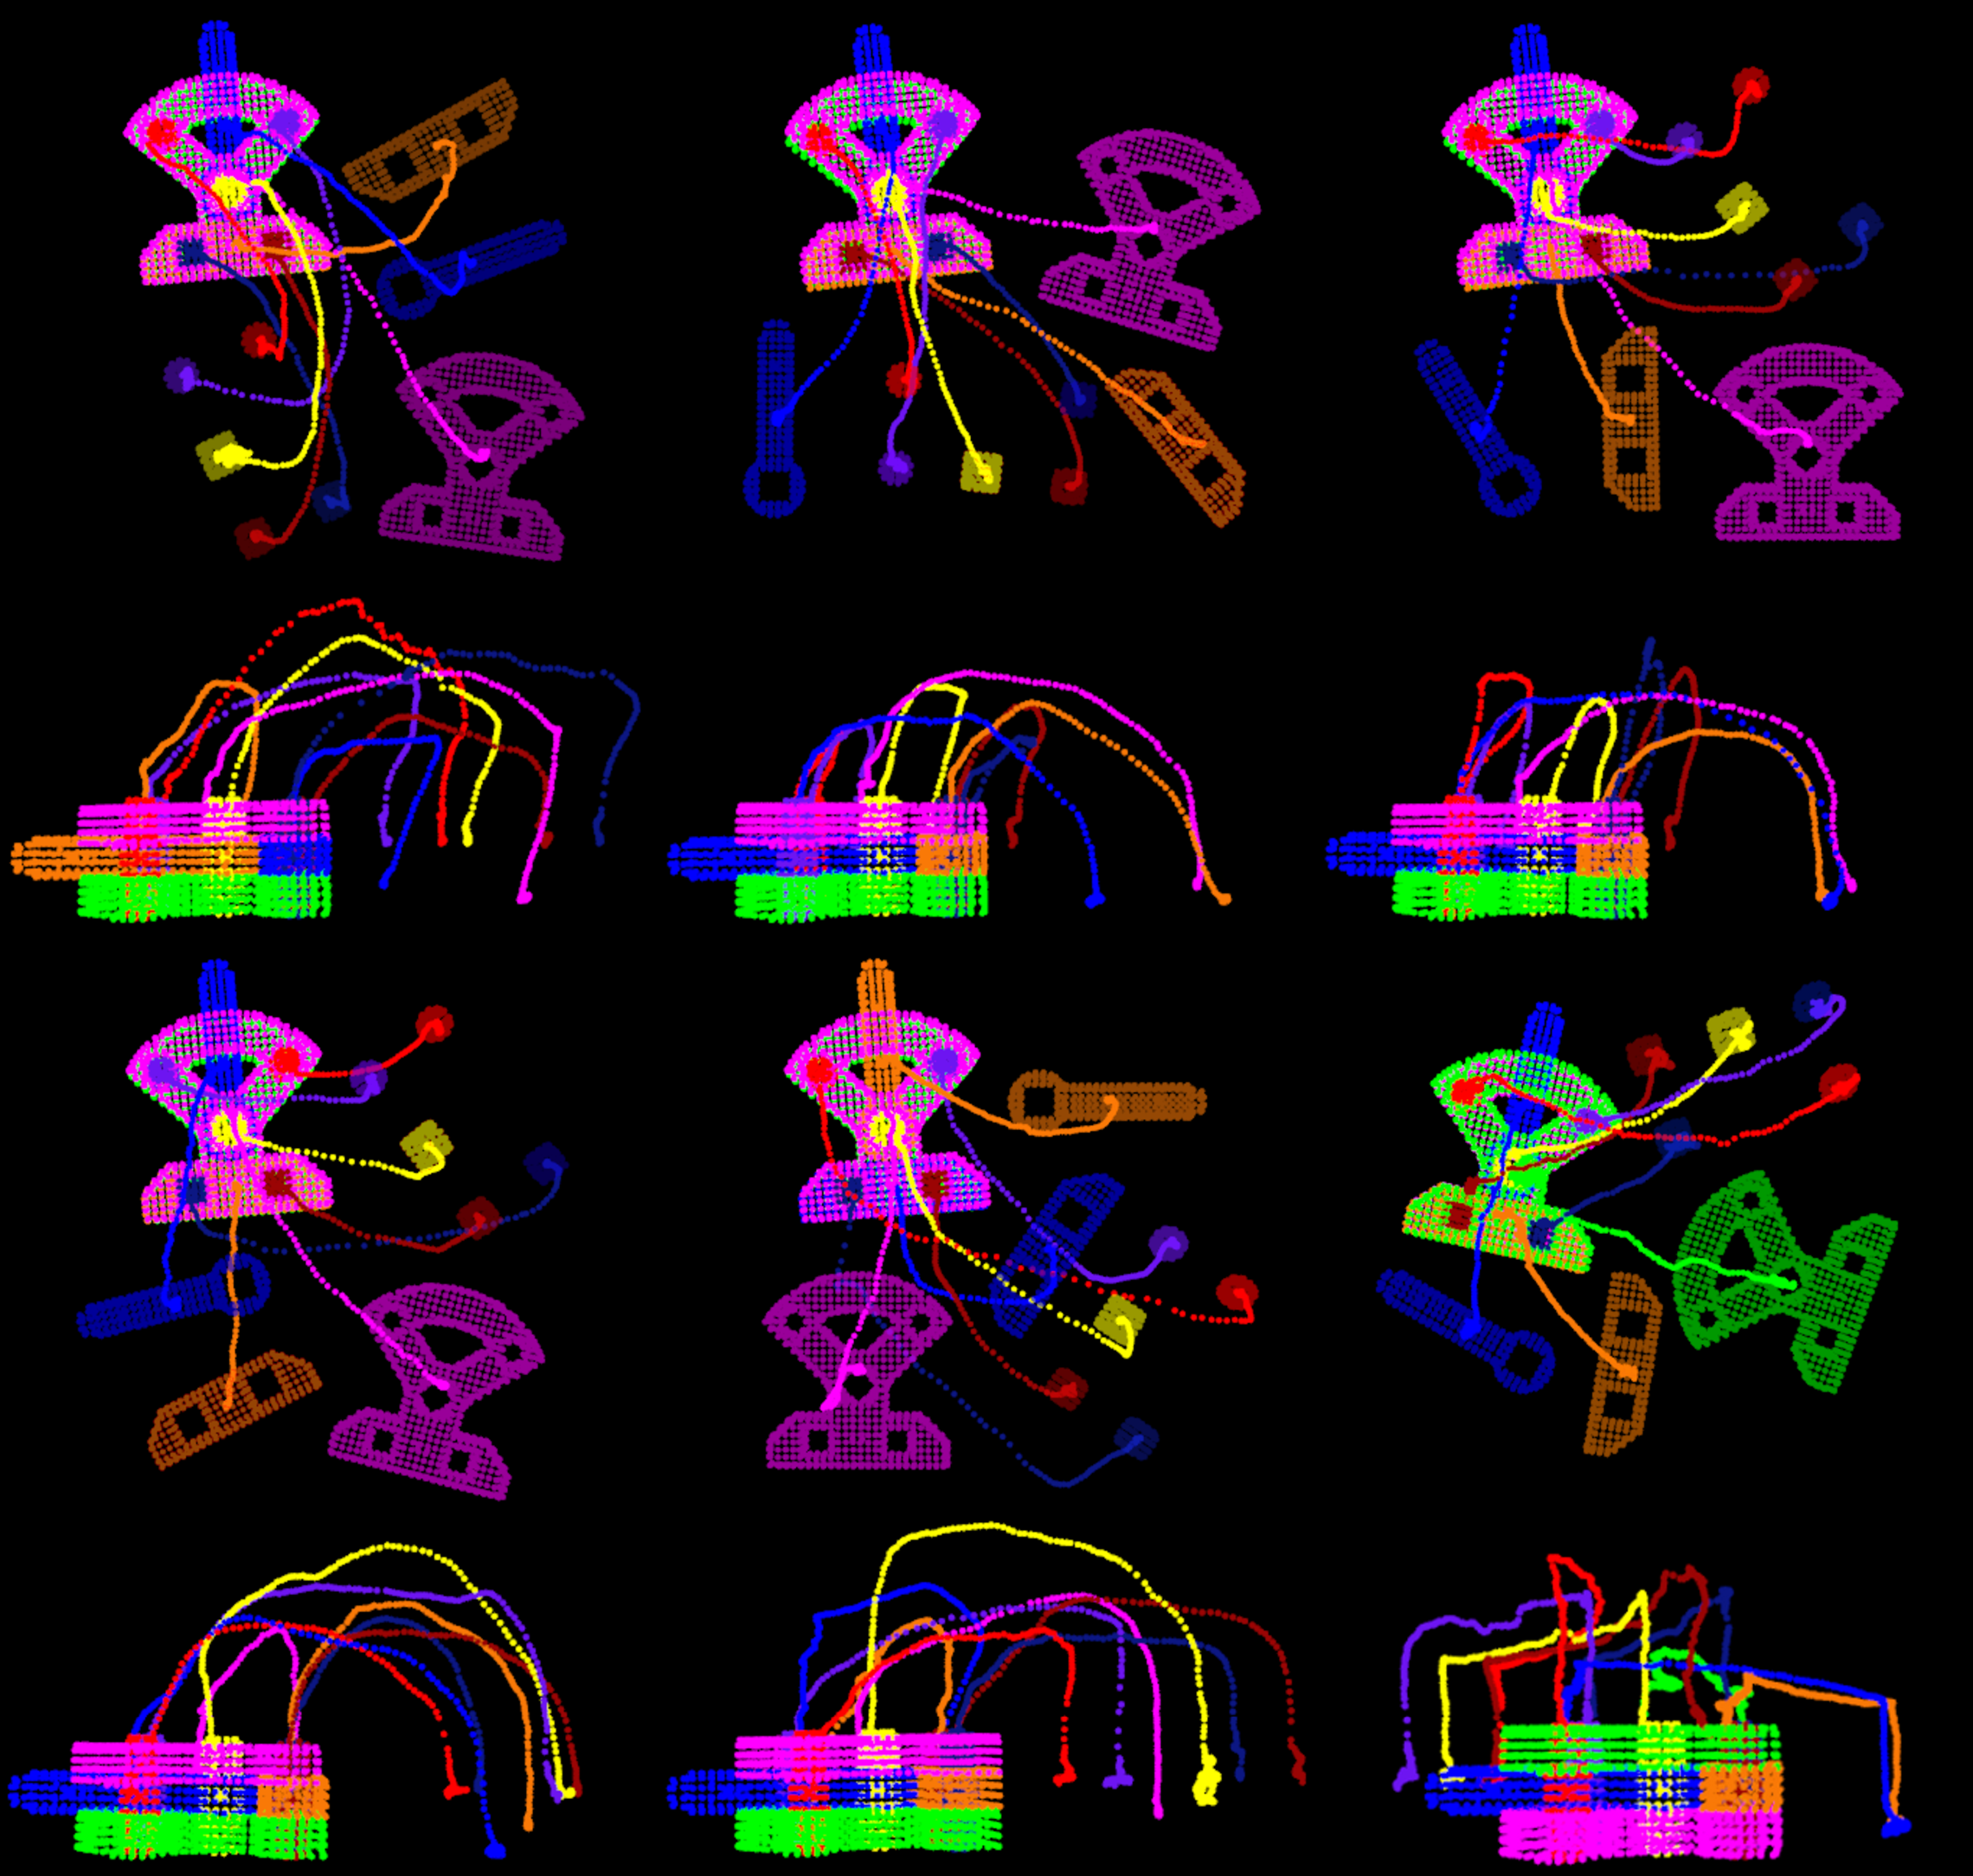
\includegraphics[width=1.0\textwidth]{figures/Tracking/TracksMontage.pdf}
  \caption[Snapshots from Virtual Reality Benchmark Run]{Tracking results from six different recordings of the Cranfield Scenario. The tracks in the bottom right corner are from the robot constructing the object, while the other five are from five different human demonstrators. In the overhead views, starting poses are shown (in slightly darker colors) for the objects.}
  \label{fig:TrackingResults}
\end{figure*}

\section{Discussion}
In this Chapter we have presented a novel spatially stratified sampling approach which greatly reduces the computational complexity of 3D Point Cloud correspondence particle filters. We evaluated the tracker using synthetic sequences for which precise ground truth exists, as well as real sequences of a human demonstration application. To demonstrate the effect of stratified sampling on performance, we conducted a sweep over the parameter space of number of particles and samples. This sweep showed the clear effectiveness of the proposed method in matching and even out-performing a GPU implementation. 

The approach we have presented here allows us to effectively track rigid objects in 3D voxel space. While it is very efficient at doing this tracking, it remains just that, a tracker, the result of which is an object state. Moreover, it is unable to handle deforming objects, and as of yet we have not shown how to handle objects entering or leaving the scene. That is to say, we have yet to show how we can use this tracking system to produce a full video segmentation.

As such, now that we have now established our ability to track multiple objects in real-time within point cloud data, we can proceed to \gls{vos}. In the next Chapter, we will combine the 3D correspondence-based tracker with the supervoxel world-model presented previously to generate a full segmentation of point cloud video that is robust to occlusion and maintains object identities throughout extended sequences. To do this, we shall borrow some ideas from our 2D tracker presented in Chapter~\ref{Chap:VideoSegRelaxation}, and introduce a new global energy function that allows us to assign newly observed supervoxels to tracked targets.


\begin{savequote}[75mm]
Problems worthy

of attack

prove their worth

by hitting back. 
\qauthor{Piet Hein}
\end{savequote}

%For an example of a full page figure, see Fig.~\ref{fig:myFullPageFigure}.

\chapter{Tracking Based Point Cloud Video Segmentation}
\label{Chap:TrackingBasedSegmentation}
\lettrine[lines=3, loversize=0.3]{\textcolor{DarkBlue}S}{o far, we have presented} a 2D particle-filter based VOS method, developed a 3D point-cloud based world-model, and shown how it is possible to efficiently track within this model using particle filters. Our final task is to bridge the gap between the tracked models from the previous Chapter and the supervoxels presented in the preceding one. Connecting the two will allow us to track at the supervoxel (rather than object) level. 

The reason for tracking supervoxels rather than objects is a practical one - what we define as an ``object'' is largely dependent on context, as it is really a property of the observer, rather than the observed. By tracking supervoxels we can avoid the problem of having to make strict decisions defining object boundaries at each time step. Instead, we make ``fuzzy'' associations, where instead of a binary association decision, we instead maintain probabilities that supervoxels ``belong'' to different objects.

There are many avenues available to proceed in doing this, and which one is optimal remains an open question. In this Chapter we shall describe the avenue which we pursued, show our results, and discuss where future research should lead. We should note that the research presented in this Chapter is on-going, and while we present our current results, we hope to expand the system to be more flexible in the future.

Before we begin, it will probably be helpful if we show visually exactly what we are trying to achieve. Figure \ref{fig:TODOFIGURE} gives such an outline; the core idea is that we want to propagate supervoxels forward through time.  While the tracking we presented in the previous Chapter estimates a 6DoF pose for models in each frame, we now want to use tracked results to find a temporal association for each supervoxel. The advantage of using tracking to accomplish this is its ability to maintain object identities through occlusions, sudden movements, and other difficult situations - as well as to avoid the so-called ``aperture'' problem. 

\todo[inline]{Figure showing supervoxels, tracked models, associations to achieve segmentation}

\section{Tracked Model Representation}
The first issue that must be addressed is the ``level'' at which targets should be tracked - the object or the supervoxel level (we shall not consider tracking at the voxel level since it is computationally infeasible with current hardware). As our goal is to associate supervoxels across time, we would like to track supervoxels directly. Unfortunately, this is generally not feasible due to the ``aperture problem'' seen in neural visual fields~\cite{MarrApertureProblem}. The aperture problem deals with the fact that local motion can only be estimated perpendicular to a contour that extends beyond its field of view~\cite{shimojo1989}. In other words, determining direction of motion in a local region (without considering global features) is generally not possible - as illustrated in Figure \ref{fig:TODOFIGURE}. This means that in order to estimate motion of supervoxels, we must extend the field of view considered significantly beyond the size of the supervoxel itself; in fact, our aperture must contain the borders of the moving object in question, otherwise pairwise association of supervoxels is generally indeterminate. 

\todo[inline]{Figure showing aperture problem? Barber pole}

To avoid this problem, we must track higher level groupings - groupings that extend at least to a contour which provides a reference boundary for disambiguating motion. A natural way of doing this is to use the LCCP segmentation presented in Chapter \ref{Chap:WorldModel}, as it will expand regions up to concave boundaries. Using concave connections as references is surprisingly powerful, as it generally will differentiate objects, as well as parts of objects which can move independently (consider the case of joints in the human body). As such, we adopt a simple scheme for grouping supervoxels into tracked models; we perform LCCP segmentation on the first frame, and assign each observed segment to an independent tracker.

\section{Supervoxel-Based Particle Filters}
Tracking of the segmented models is accomplished using a bank of the correspondence-based particle filters from the previous Chapter. As our models now consist of supervoxels, so too must our observations - thus we use the supervoxels produced using the persistent scheme discussed in Chapter~\ref{Chap:WorldModel}. The observation model measures distance in a feature space of spatial distance, normals, color (in HSV space), and labels. Weights of predicted states $\mathbf{x}^j_t = [d_x, d_y, d_z, \gamma, \beta, \alpha]$ are measured by associating supervoxels from the transformed models to the observed supervoxels nearest in space. Particles are then weighted by measuring total distance in feature space, just as in (\ref{eqn:distance}), with the addition of a binary label term,
\begin{equation}
  \label{eqn:dist_labels}
    W_L =  \begin{cases} 1, & L_p = L_{p^*} \\ 
                         \frac{N_k-1}{N_k}, & L_p \neq L_{p^*} 
           \end{cases} 
\end{equation}

which results in the augmented distance function

\begin{equation} \label{eqn:augmented_distance}
  \tilde{w}^j = \sum_{1}^{\eta} \frac{1}{1 + \frac {\mu \lVert \mathbf{p}^j_{xyz} - \mathbf{p}^*_{xyz} \rVert} {R_{voxel}} +  \frac{\lambda D_c(p^j_{RGB},p^*_{RGB})}{m} +   \epsilon \lVert \mathbf{p}^j_{n_x n_y n_z} - \mathbf{p}^*_{n_x n_y n_z} \rVert + \nu  W_L}.
\end{equation}

As before, we adopt the notation $p$ for the supervoxel and $p*$ for its corresponding supervoxel in the observation.

\section{Association by Joint Energy Minimization}
The additional step that we must take to extract a full segmentation (rather than only object tracks) is to associate the observed supervoxels to the predictions coming from the particle filters. That is, we must connect the tracked outputs back to the observations, and make a per-voxel association, solving the multiple target data association problem. We do this using an energy function scheme which seeks to find a global labeling of supervoxels which minimizes our global  . To do this, we first create a list of all observed supervoxels which lie within a radius $R_{seed}$ of each predicted supervoxel coming from the particle filters (see Fig.~\ref{fig:Association}). Then we select all supervoxels which could only be associated with one possible object, associate them, and remove them from further consideration.

\begin{figure}[tb]
  \centering
  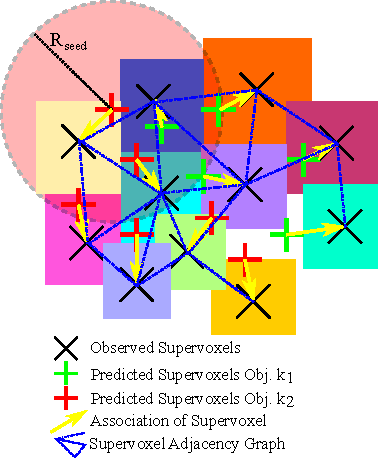
\includegraphics[scale=1.0]{figures/IROS2013/Association.pdf}
  \caption[Supervoxel Association]{Association of observed supervoxels with predicted model supervoxels using global energy.}
  \label{fig:Association}
\end{figure}

To associate the remaining observed supervoxels, we determine which objects are competing for them, and then find the predicted supervoxel from each object which lies closest to them in the feature space (using spatial location, normals, and color as in (\ref{augmented_distance})). We adopt a RANSAC-like approach, similar to \cite{EnergyBasedMultiModel}, to sample from the set of possible associations and determine a global association which best aligns the predictions to the observed supervoxels. Additionally, we use a weighted sampling strategy where the likelihood of assigning object $k$ as the label $L$ of supervoxel $p$ falls off with increasing distance from the object centroid $C_k$
\begin{equation}
 \label{eqn:WeightSampling}
 \mathcal{L}(L_p=k | C_k) = \frac{1}{C_k}.
\end{equation}

To score a set of assignments, we compute a global energy, given in~(\ref{eqn:Energy}). Each global label association $\mathcal{A}$ consists of local associations $a$ which assign an object label $k$ to each observed supervoxel $p$. The first summation term, $ \sum_{p}{\|p^*_k - p\|} $, measures error in feature space between the observed supervoxel and the closest supervoxel in its associated predicted object $p^*_k$. 

\begin{equation}
\label{eqn:Energy}
{E}_\mathcal{A} =\prod_{a\in\mathcal{A}}{\Delta_k} \left( \sum_{p}{\|p^*_k - p\|} + \lambda \sum_{(p,p')\in \mathcal{N} }\delta(L_p \not= L_{p'}) \right) 
\end{equation}

The second summation is a smoothing prior which considers the adjacency graph of observed supervoxels. For every observed supervoxel, we compare its assigned label $L_p$ to the label of all supervoxels $p'$ which lie within its adjacency neighborhood $\mathcal{N}$. We adopt the Potts model as in \cite{Boykov2001}, where $\delta(\dot)$ is 1 if the specified condition holds, and 0 otherwise, and $\lambda$ is a weighting coefficient which controls the importance given to spatial continuity of labels.

Finally, the multiplicative term $\prod_{a\in\mathcal{A}}{\Delta_k}$ controls for the expansion or contraction of object volumes through the number of observed supervoxels associated with them. $\Delta_k$ penalizes for changes in volume by increasing the energy for deviations from unity in the ratio of observed supervoxels assigned to an object $\hat{N}_k$ with the number in the object model itself $\hat{N}_k$, that is

\begin{equation}
\label{eqn:DeltaSVs}
\Delta_k = \left\{ 
  \begin{array}{l l}
    {\hat{N}_k}/{N_k} & \quad \text{if ${\hat{N}_k} \geq {{N}_k}$ }\\
    2 - {\hat{N}_k}/{N_k} & \quad \text{if $\hat{N}_k < {N}_k$}~. 
  \end{array} \right.  
\end{equation}

Once the energy arrives at a stable minimum, we extract the resulting association of observed supervoxels to predicted results, and use them to update the tracked models.

\begin{figure*}[!ht]
  \centering
  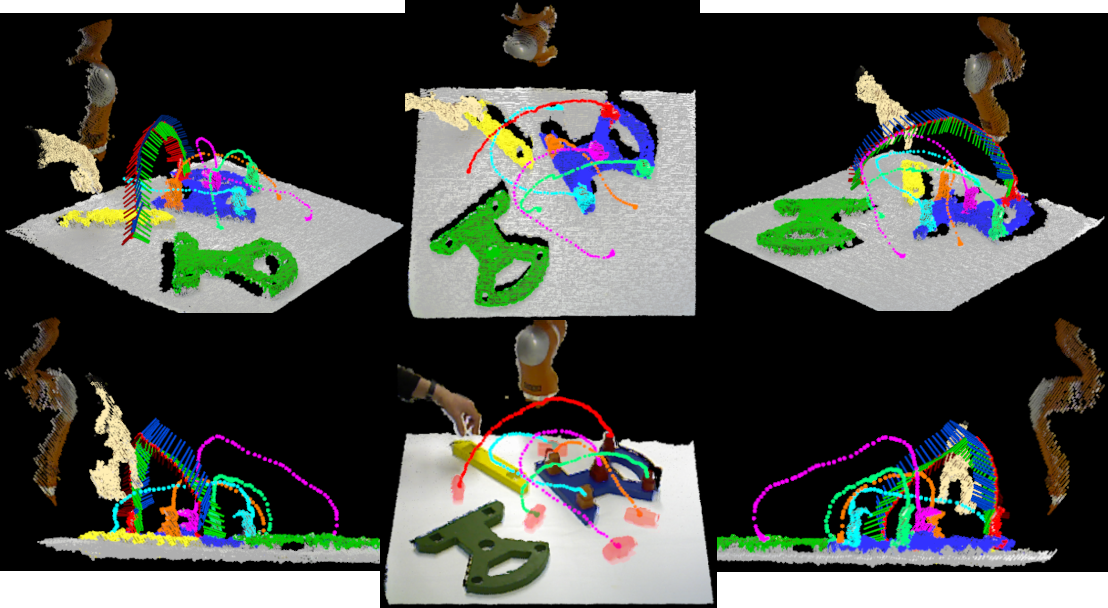
\includegraphics[width=\linewidth]{figures/IROS2013/TrajectoriesNew.pdf}
  \caption[Cranfield Tracking Results]{Result of tracking and segmentation on Cranfield scenario from different views. Here the tracks are shown as dots of the color of the tracked label for each timestep. Initial locations of the pegs are shown in the middle bottom frame as semi-transparent masks. Calculated orientation is shown for the red peg with a set of axes every second time-step; these axes show pose in a frame relative to the start. }
  \label{fig:Trajectories}
\end{figure*}

\section{Alignment and Update of Models}
The joint energy minimization results in a global association $\mathcal{A}$ which assigns observed supervoxels to tracked objects. In order to use this to update the object models, we determine a transform which aligns it to the internal representation stored by the particle filter. As an initial guess, we use the inverse of the predicted state, and then use an iterative closest point \cite{ICPChetverikov} procedure to refine the transform such that the set of observed supervoxels best aligns with the model prior. We then replace the model prior with the new observed supervoxels. 

As a final step, we use the refined transform to update the states of the particles. To do this, we shift each particle $x_i$ towards the refined state $\hat{x}$, weighting the importance given to the refined state by a constant factor $\epsilon$

\begin{equation}
\label{eqn:PFUpdate}
x'_{i \in L} = (1-\epsilon) x_i + \epsilon \hat{x}~.
\end{equation}

For this work, we found that an $\epsilon$ of $0.5$ effectively removes noise (jitter) introduced by the replacement of the tracked model. Additionally, we correct the internal motion model of the particle filters to correspond to the new updated state.

\section{Experimental Results}
In order to demonstrate the usefulness of the proposed method, in this Section we first provide results from two successful applications. Both applications use the Cranfield scenario \cite{collins1984development} as in the previous chapter. Figure~\ref{fig:Trajectories} show the results of tracking and segmentation (only the pegs are shown in Figure~\ref{fig:Trajectories} to avoid clutter) using our Cranfield pieces. It can be seen that the algorithm is able to successfully extract full segmentation throughout the video.

%%%%%%%%%%%%%%%%%%%%%%%%%%%%%%%%%%%%
\subsection{Imitation of Trajectories for Robot Manipulation}
\begin{figure}[!tb]
  \centering
  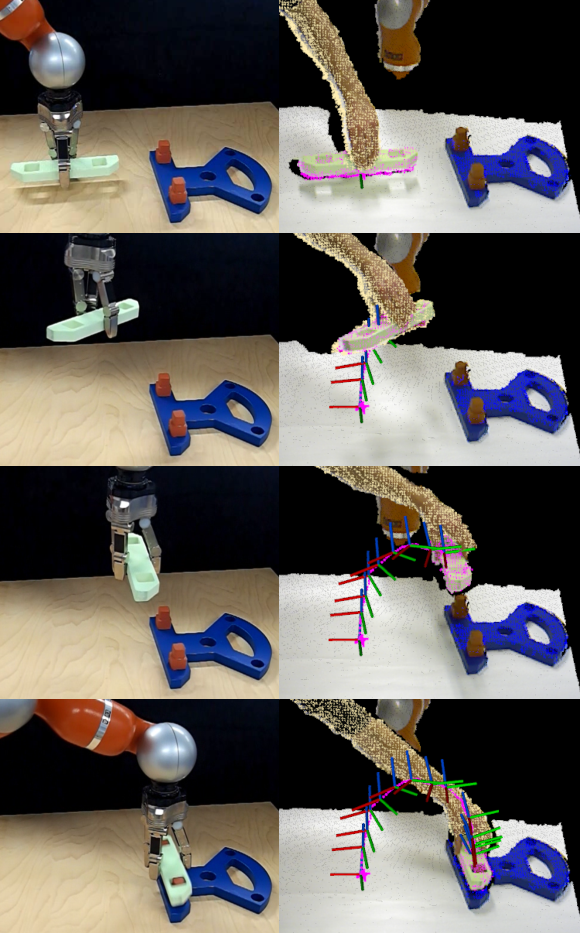
\includegraphics[scale=0.84]{figures/IROS2013/RobotImitation.pdf}
  \caption[Trajectory Imitation]{Kuka LWR arm imitating trajectory and pose learned from tracked human demonstration.}
  \label{fig:Imitation}
\end{figure}
The standard way of teaching robots to perform human-like actions is imitation learning, also called programming by demonstration \cite{Billard2008,Argall2009}. There are several ways to demonstrate movements: 1) recording movements in joint-space (joint angles) or target-space (Cartesian space) by ways of a motion capture device (requires putting markers on human body), 2) using kinaesthetic guidance (guiding a robot's movements by a human hand), or 3) via teleoperation (controlling a robot via joystick). The only way to obtain motion trajectories from human observation in a "non-invasive" procedure is by using stereo vision \cite{Hecht2009}, however, usually it is model based. The tracking algorithm we have presented here can be used as an alternative method to obtain motion trajectories (in Cartesian space) in a model-free way. 

To demonstrate this, we applied our tracking algorithm to obtain human motion trajectories in Cartesian space including orientation of manipulated object (in total six DoFs). We tested it using a recording of the Cranfield scenario where, first, we let a human demonstrate the action and then reproduced it using a KUKA Light Weight Robot (LWR) arm \cite{kuka}. Specifically, here we imitate a human putting the separator block on the pegs. To generate trajectories for the robot from human demonstrations, we used a modified version of Dynamic Movement Primitives \cite{Ijspeert2002,Ijspeert2013} (DMP) and learning method as described in \cite{Kulvicius2012}. We used Cartesian impedance control and, thus, generated six DMPs (three for motion of the end-effector in Cartesian space and three for orientation of the hand) based on trajectories obtained from the tracking algorithm. Here we used 100 equally spaced kernels with width $\sigma=0.05$ for each dimension (for more details please refer to \cite{Kulvicius2012}).
 As demonstrated in Fig.~\ref{fig:Imitation} and the supplementary video, trajectories obtained by the proposed tracking algorithm are sufficiently accurate to allow reproduction of the human motion.

%%%%%%%%%%%%%%%%%%%%%%%%%%%%%%%%%%%%

\subsection{Semantic Summaries of Actions}
\todo[inline]{Need to show results on Eren's action recordings instead, but how to show it makes a difference. Maybe use it to do object classification at the end based on what the tracked action was? Or just say we generate SECs without needing object models.}

A fundamental task for intelligent autonomous robots is the problem of encoding long chain manipulations in a generic way, for use in tasks such as learning and recognition. As a demonstration of the usefulness of the proposed tracking framework, we use a recently introduced novel Semantic Event Chain (SEC) approach \cite{Aksoy11} which converts each segmented scene to a graph: nodes represent segment (i.e. object) centers and edges indicate whether two objects touch each other or not. By using an exact graph matching technique the SEC framework discretizes the entire graph sequence into decisive main graphs. A new main graph is identified whenever a new node or edge is formed or an existing edge or node is deleted. Thus, each main graph represents a “key frame” in the manipulation sequence. Figure~\ref{fig:SECGraphs} shows a few detected sample key frames from the long Cranfield action. While the complete action has in total 1453 frames, the SEC representation reduces it to just 35 key frames, each of which represents a topological change in the scene.

\begin{figure*}[ht!]
  \centering
  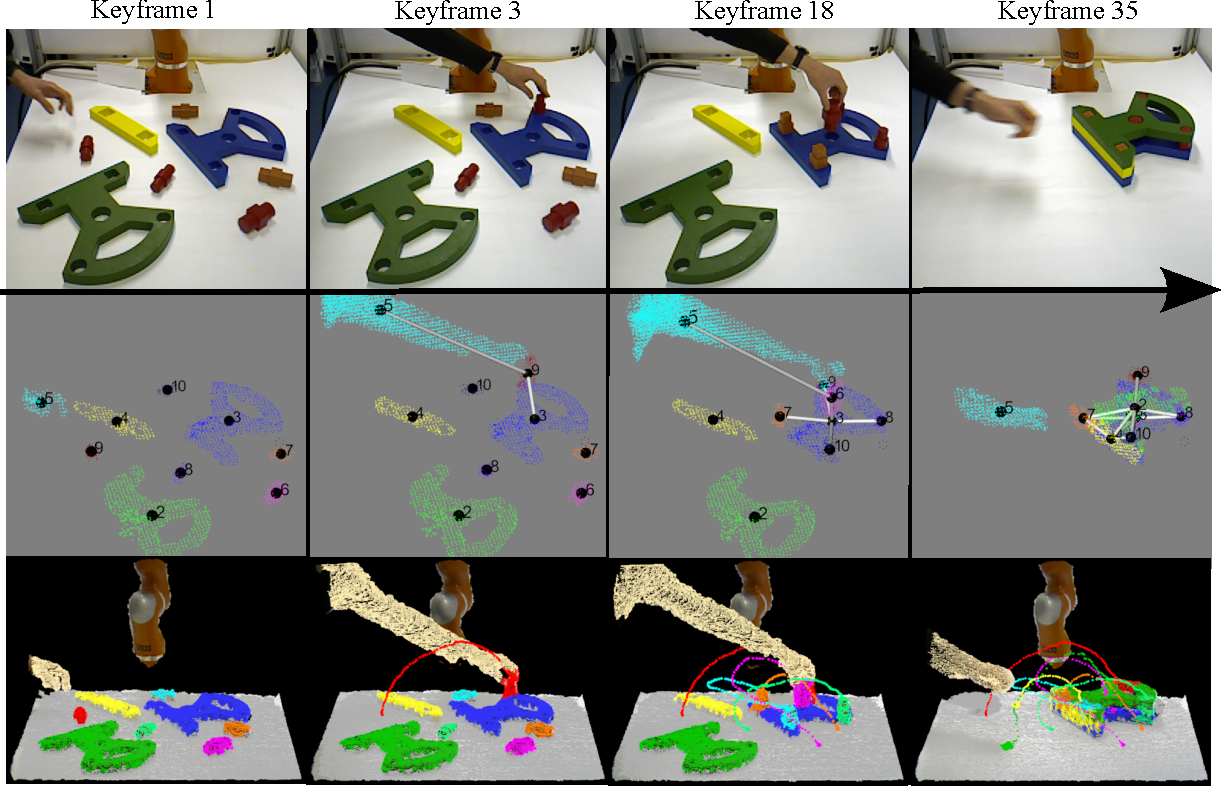
\includegraphics[width=\linewidth]{figures/IROS2013/SECKF.pdf}
  \caption[Cranfield Key Frames]{A few example key frames extracted from the long Cranfield action. Numbered nodes represent interacting objects, while edges show touching relations between objects. Each keyframe represents a topological change in the scene - here we show 4 of the 35 keyframes.}
  \label{fig:SECGraphs}
\end{figure*}
\begin{savequote}[75mm]
Some Quote.
\qauthor{Quoteauthor Lastname}
\end{savequote}

%For an example of a full page figure, see Fig.~\ref{fig:myFullPageFigure}.

\chapter{Conclusions}
\label{Chap:Conclusions}
\newthought{There's something to be said} for having a good opening line. 
\section{Summary and Contributions}
\section{Directions for Future Work}
\section{Discussion of Limitations of Benchmarks}




%% Requires fltpage2 package
%%
% \begin{FPfigure}
% \includegraphics[width=\textwidth]{figures/fullpage}
% \caption[Short figure name.]{This is a full page figure using the FPfigure command. It takes up the whole page and the caption appears on the preceding page. Its useful for large figures. Harvard's rules about full page figures are tricky, but you don't have to worry about it because we took care of it for you. For example, the full figure is supposed to have a title in the same style as the caption but without the actual caption. The caption is supposed to appear alone on the preceding page with no other text. You do't have to worry about any of that. We have modified the fltpage package to make it work. This is a lengthy caption and it clearly would not fit on the same page as the figure. Note that you should only use the FPfigure command in instances where the figure really is too large. If the figure is small enough to fit by the caption than it does not produce the desired effect. Good luck with your thesis. I have to keep writing this to make the caption really long. LaTex is a lot of fun. You will enjoy working with it. Good luck on your post doctoral life! I am looking forward to mine. \label{fig:myFullPageFigure}}
% \end{FPfigure}
% \afterpage{\clearpage}



\singlespacing

% the back matter
\clearpage
\bibliography{IEEEabrv.bib,PaponRefs.bib,references.bib,IROS2013.bib,ECCV2012.bib}
\addcontentsline{toc}{chapter}{References}
\bibliographystyle{plainnat}
%\include{endmatter/colophon}

\onehalfspacing

\begin{appendices}
%For an example of a full page figure, see Fig.~\ref{fig:myFullPageFigure}.
\graphicspath{{figures/Oculus/}}

\chapter{The Oculus Vision System}
\label{chap:Oculus}
\section{Motivation}
There is great interest in development of complex vision systems for robotic vision applications. Such research has strict requirements; these systems must operate in real-time, using input from multiple sources, and typically consist of multiple algorithms which work in concert to produce useful output with minimal delay. Consequently, the architecture which binds algorithms and input sources together has become an increasingly important factor. In this Appendix we shall present a vision architecture we developed over the course of the thesis work which uses modular plugins, a novel buffering scheme, and GPU memory optimizations to allow real-time performance of an online vision system, even with complex pipelines and algorithms developed by independent researchers.

A primary concern when developing such complex vision systems lies in how to properly integrate algorithms developed by different researchers, often from multiple institutions. Typically, computer vision researchers develop solutions tailor-made for their particular problem, without concern over the difficulties involved in integrating their particular algorithm into a large system. To ease this integration process, we provided a plugin interface. The plugin system allows independently developed algorithms to communicate with the architecture's central memory management system, interact with the GUI, define their own unique data types, and integrate into systems with plugins developed by other researchers.

Another motivation for developing a vision architecture is the desire to enable the use of complex algorithmic layouts in an online system. In particular, interest in creating loops that allow high level algorithms (i.e. which come late in the pipeline) to feedback and improve the output of low level vision methods. Traditional online vision pipeline architectures cannot accommodate such loops in an adequate way, as at any given moment each portion of the pipeline is processing data from different instants in time. 

Existent vision system architectures also do not support the use of GPUs in a fully integrated way, leading to inefficient use of the device and communication with device memory. The presented method incorporates specially designed GPU data-containers to ensure optimal PCI-bus use through a pre-caching scheme and concurrent memory transfers. In addition to these, extensibility is ensured through an interface which allows user-defined data-container handling, allowing plugin developers to explicitly define how the memory manager shares data between the host and device. In this Appendix we will present an overview of our system, describe a typical system configuration used for robotics, and then give performance figures from a demonstration setup.

%\section{Related Work}
%The most widely used vision software in the field is the OpenCV library, thanks to its permissive license, active development, and large gamut of algorithms. While useful in accelerating the creation of algorithms, OpenCV lacks many of the tools needed for construction of a complete vision system \cite{CVFrameworks}. In particular, OpenCV has limited visualization support, lacks a framework for constructing complex streaming pipelines, and has only recently begun adding GPU support. 
%There are a few existing open-source projects centered around computer vision system architecture, such as iceWing \cite{Icewing} and Imalab \cite{Imalab}. These systems bear some similarities to ours, in that they are sophisticated vision development environments, featuring modularity, efficient visualization, and simple control of algorithm parameters. While a step forward, these projects lack two core features required for our work; support of feedback loops and integrated use of the GPU as a coprocessor. 
%In addition to the open-source projects, there are a few commercial solutions available. Foremost among these is MATLAB, which uses a high-level scripting language to allow for rapid development. Unfortunately, its restrictive and expensive licensing can make it difficult to develop algorithms in distributed locations; every developer must have not only a MATLAB license, but also licenses for the multiple toolboxes required. Additionally, since MATLAB (and it's open source equivalent Octave) development is not in C/C++, creation of novel GPU algorithms using a language such as CUDA is difficult. Other commerical solutions, such as HALCON \cite{HALCON} or BLOX \cite{BLOX} also suffer from their restrictive licensing, making them not well suited for research. None of these solutions permit feedback loops in a real-time online vision system.

%%%%%%%%%%%%%%%%%%%%%%%%%%%%%%%%%%%%%%%%%%%%%%%%%%%%%%%%%%%%%%%%%%%%%%
%%%%%% SYSTEM ARCHITECTURE %%%%%%%%%%%%%%%%
%%%%%%%%%%%%%%%%%%%%%%%%%%%%%%%%%%%%%%%%%%%%%%%%%%%%%%%%%%%%%%%%%%%%%%
\section{System Architecture}

Our vision system is a plugin shell which provides an easy-to-use API for interacting with the GUI, memory management system, and visualization components. In order to ensure expandability, such a system must provide straightforward communication and interaction between plugins created independently, while employing strong-typing checks to ensure only valid plugins may be inter-connected. In addition, it must ensure that plugins have the flexibility to define their own methods for visualization. Finally, the system must ensure that each plugin is self-contained, and executes within its own thread (or threads). This is especially important for fast execution on modern processors, where the number of cores can match, or even exceed, the number of plugins one is running. 

In the next subsections, we shall describe how our architecture accomplishes these goals while requiring as little computational and communication overhead as possible. Small overhead is especially important in the case of real time video processing, where relatively large images must be processed at fast frame rates. 

\subsection{Execution Flow}
At its core, the architecture provides a shell which consists of a GUI for loading plugins and visualizing data, a system for storing plugin output to file, and a buffering/memory-management system for handling data. This functionality is contained in the \emph{Main Thread} and \emph{Memory Manager Thread} shown in Figure~\ref{fig:SystemArchitecture}. Users build their system by adding plugins, configuring their options via the GUI, and then connecting the plugins to each-other. The user can also save/load a fully configured system as an XML file. Once a vision system has been built, the user can control execution using the frame rate module, which controls the firing rate of the system clock. 

As the whole system runs asynchronously in independent threads, the clock trigger acts as the initial starting point for each frame. This means that any source plugins, such as a stereo camera rig or a video file reader plugin, must connect to the frame rate module. As a trigger arrives at each plugin, a triggering signal is sent to the memory manager, telling it to generate a \emph{DataContainer} for the plugin's output. The plugin is then triggered, causing it to execute its processing functionality and generate output, which it stores in the location assigned to it by the memory manager. The plugin then generates another triggering signal, which is connected to both the memory manager and whatever ensuing plugins use the output as their input. When a plugin has multiple inputs, it will loop inside its execution thread, waiting until all inputs for a frame have arrived before executing. This is accomplished by each thread having its own input queue map; it is important to note though, that these queues 
contain no actual data (and thus minimal overhead), and merely serve as a message passing system. The signaling and triggering system employs the open-source Qt signal \& slot architecture. In particular, the system makes use of Qt's ability to queue signals for execution as they arrive at a thread. 

 \begin{figure*}
\begin{center}
\includegraphics[width=165mm,height=100mm]{SystemFlowColor.pdf}
\includegraphics[width=170mm,height=112mm]{SystemOutput.pdf}
\end{center}
  \caption[Overview of the system architecture]{Overview of the system architecture and demonstration system output for four frames. The colums show output from the different components; from left to right, Kinect image and depth (in mm), optical flow, and graphs overlaid on segmentation plugin output. This type of output can be seen live in any number of visualization windows within the GUI.}
\label{fig:SystemArchitecture}
\end{figure*}

\subsection{Plugin Development and Interaction}
The functionality of the system is provided primarily via plugins. A plugin consists of a shared library which is loaded dynamically at run-time. The system is based on the low-level Qt plugin API, which facilitates development and ensures compatibility across different platforms. Plugins inherit from a pure abstract interface class which defines a protocol for communicating with the core application. This permits plugins to define input and output types and pass messages to/from the GUI and memory manager. 

Developers are required to implement a \emph{processData} function, which receives input and writes to an output \emph{DataContainer}. The developer can optionally create any number of GUI elements (e.g. sliders, buttons) using the interface functions.  Plugins specify how many inputs they require, and give the possible types for these inputs. Communication between plugins is accomplished through a standardized data container interface. The core architecture contains commonly used data container implementations, such as \emph{StereoImageContainer}. Plugins may define their own specialized data containers which are loaded at runtime with the plugin. For example, the Segmentation plugin has its own container type \emph{SegmentationData}, which contains a list of labeled segments, metadata about the segments, and labeled images. The standardized data container interface allows for any plugin to refer to a new container class without actual knowledge of the container itself other then the string identifiers of 
its members (e.g. "Segment Labels"). Correct handling of access to these members is accomplished through dynamic dispatch using the virtual lookup table. This ensures that a plugin written by one researcher can be easily used as input to another's, as long as they know the proper identifiers and underlying formatting of the data. 


\subsection{Visualization}

During the development and use of a vision system, it is of utmost importance to be able to visualize what is occurring at every stage of the system pipeline. As such, our system allows users to create any number of visualization windows which can select any plugin to display (and which part of the plugin's output to display, e.g. left or right image). If a developer creates their own data container for a plugin, they can define a special visualization callback function as part of this container. The system will automatically detect this callback when the plugin is loaded, and use it for visualizing the plugin's output. Developers can specify multiple methods for visualizing the plugin; the GUI for visualization will allow selection of which to display.

Visualization windows read directly from the global buffer, and as such have a small memory overhead. Additionally, visualization runs in the GUI thread, rather than in any of the plugin threads. If a plugin slows down the system, visualization (and the GUI) will remain responsive, allowing the user to troubleshoot. This also means that visualization that requires computation, such as labeling an image with text or vector graphics, will have a negligible effect on the actual frame throughput of the system. If visualization lags behind the system output, frames are automatically skipped on an interval that allows visualization to maintain synchronization with the rest of the system. This is of particular importance in an online system, such as our real-time robotic application, where visualization lagging behind processing can cause confusion or even errors.

%%%%%%%%%%%%%%%%%%%%%%%%%%%%%%%%%%%%%%%%%%%%%%%%%%%%%%%%%%%%%%%%%%%%%%
%%%%%% MEMORY ARCHITECTURE %%%%%%%%%%%%%%%%
%%%%%%%%%%%%%%%%%%%%%%%%%%%%%%%%%%%%%%%%%%%%%%%%%%%%%%%%%%%%%%%%%%%%%%

\section{Memory Architecture}
The memory management system has been designed to allow distributed development and computing, complex system pipelines incorporating feedback loops, and efficient use of the GPU as a computational resource. The following subsections will describe how these design goals have been achieved by illustrating our \emph{Global Buffer} design and explaining how it manages GPU memory.  

\subsection{Global Buffer}
Our global buffer concept was designed to overcome the limitations of standard online vision pipelines. In a standard online pipeline a local buffering scheme is used; each algorithm has an input buffer, where data accumulates while it is waiting to be processed. Such a setup is adequate as long as the  pipeline remains unidirectional, but complications arise in using feedback loops.
\begin{figure}[t]
\begin{center}
   \includegraphics[width=0.6\linewidth]{BufferComparaison.pdf}
\end{center}
   \caption[Comparison of Buffering Schemes]{A typical buffering scheme (top) and our buffer (bottom).}
\label{fig:BufferFig}
\end{figure}
Figure~\ref{fig:BufferFig} compares a standard pipeline with our global buffer; unlike a typical buffering scheme, our global buffer maintains and manages all memory in a central location (and separate thread). The global buffer is responsible for dynamic allocation of all data containers, maintaining reference counts, and determining when a frame can expire. Since the global buffer is responsible for maintaining memory, plugins use a message passing system to communicate. Plugins pass messages to each other to notify completion of a new frame, or to trigger a feedback mechanism. They also use the message passing system to request that the global buffer allocate a new data container for their output. When a developer creates a new type of data container, they use a simple interface to pass the global buffer a function pointer for creating an instance of their new data container type. 

In order to fully understand the limitations of a standard buffering system, consider, for instance, the system shown at the top of Figure~\ref{fig:Feedback}.  If the feedback mechanism is triggered for frame \emph{n}, plugin \emph{B} must return to frame \emph{n} in order to modify how it was processed. This is not possible in the standard local buffer scheme, as that data was discarded after it was used as input to \emph{B}. One possible solution is to maintain another local buffer for each plugin which contains data which has already been processed, but this quickly adds several degrees of complexity. In particular, garbage collection becomes very difficult, and management of these buffers when feedback does occur becomes unnecessarily convoluted.

\begin{figure}[t]
\begin{center}
\includegraphics[width=0.6\linewidth]{Feedback.pdf}
\end{center}
   \caption[Feedback using a Global Buffer]{Feedback using a global buffer}
\label{fig:Feedback}
\end{figure}

The global buffer solves this by maintaining data in a more structured way. When a feedback mechanism is triggered for frame \emph{n} the triggering plugin (\emph{D}) sends a message to \emph{B}, causing it to stop processing what it has scheduled, and revert to frame \emph{n}. As frame \emph{n} is still easily accessible in the global buffer, \emph{B} can simply send a request for the pointer(s) to the input data container(s) it requires. The global buffer is guaranteed to still have the data for frame \emph{n}, because \emph{D} never produced an output for frame \emph{n}, so the global buffer has not marked frame \emph{n} as complete. Once \emph{B} finishes processing frame \emph{n} with its new feedback information, it will overwrite its old output for frame \emph{n} (shown in orange) and then simply continue on as it would normally, processing frame \emph{n+1}. The feedback corrected data will propagate down the pipeline, and any data which is no longer valid (shown in red) will simply be overwritten. 
Infinite feedback loops are avoided by a preventing feedback from occurring more than once per plugin per frame.

\subsection{GPU Memory Handling}
While utilizing the massively-parallel GPU as a coprocessor has become increasingly common, how to integrate it effectively into an open vision architecture remains an open question. Particularly vexing is how to integrate it seamlessly into the memory system of such an architecture, as the GPU has separate physical memory, which is entirely distinct in both location and structure from that used by the CPU. Data streaming through the system must be transferred to the GPU for modules which use it, and then transferred back out for visualization and used by modules later in the pipeline.

A naive implementation of this architecture would simply serialize the operations; when a module needs to use the GPU, it copies data to device memory, executes a kernel, and then copies the output back out to host memory. While this is still relatively efficient, it fails to fully take advantage of the pipelined streaming architecture, since the memory transfer bandwidth is idle while the kernel is executing. The architecture uses the streaming CUDA API to utilize this spare bandwidth, allowing it to perform concurrent asynchronous memory transfer and kernel execution. 

\begin{figure}[t]
\begin{center}
\includegraphics[width=0.7\linewidth]{ConcurrentGPU.pdf}
\end{center}
   \caption[Streaming and Concurrent Kernels]{Streaming; Concurrent kernel execution}
\label{fig:Streaming}
\end{figure}

As shown in Figure~\ref{fig:Streaming}, we utilize a pre-caching technique, whereby data for frame~\emph{n+1} is transferred during the execution of frame~\emph{n}. When the kernel execution time is significantly longer than the transfer time (\emph{B}), memory transfer is completely hidden, even with unidirectional memory. When kernel execution time is comparable to memory transfer time, only some of the transfer can be hidden (\emph{C}), unless the hardware supports concurrent data transfers\footnote{Concurrent data transfers are supported under the Fermi architecture. Currently the Fermi Quadro and Tesla series cards have two Direct memory access (DMA) engines, allowing them to perform host-to-device and device-to-host operations simultaneously. The consumer Fermi cards (GTX 4xx, 5xx) only have a single DMA engine, so concurrent transfers are disabled on them.}  (\emph{D}).


%%%%%%%%%%%%%%%%%%%%%%%%%%%%%%%%%%%%%%%%%%%%%%%%%%%%%%%%%%%%%%%%%%%%%%
%%%%%% DEMO SYSTEM %%%%%%%%%%%%%%%%
%%%%%%%%%%%%%%%%%%%%%%%%%%%%%%%%%%%%%%%%%%%%%%%%%%%%%%%%%%%%%%%%%%%%%%

\section{Demonstration System}
This section presents a real-time demonstration system, consisting of six plugins. The demonstration system calculates dense disparity using a standard stereo camera setup (rather than Kinect data) in order to show the flexibility of the architecture as well as highlight the speedup achieved via multithreading. Switching from Kinect input to a stereo camera setup is simply a matter of changing connections in the GUI. The pipeline described consists of plugins for reading  and rectifying stereo data, calculating optical flow\cite{PauwelsArchitecture}, computing disparity\cite{PauwelsArchitecture}, segmentation and tracking\cite{Abramov_3DSegmentation}, dense disparity estimation, and semantic graph and event chain generation\cite{Aksoy2010,Aksoy2011}. This type of a system configuration is used to recognize and learn object manipulation actions in a robotics context.

\subsection{Image Acquisition}
Video is acquired using a Firewire stereo camera rig. Triggering for image acquisition can be controlled using either an external hardware trigger or the architecture's software clock. Rectification is performed on the GPU (there is a separate plugin for calibration using a standard chessboard). Time from triggering to output of a rectified pair of stereo images is around 10ms at 1024x768.
%Support for the Microsoft Kinect camera is provided via the OpenNI library \cite{openNI}, along with the NITE middleware \cite{NITE}. The Kinect is an especially attractive option as an input source, as it provides both images and high quality disparity maps synchronized at 30fps. Raw Kinect disparity is transformed to a normalized depth, and then rectified to align with the video stream~\cite{Burrus_KinectCal}.  

\subsection{Disparity and Optical Flow}
Optical flow is computed using the GPU implementation \cite{PauwelsArchitecture} of a phase-based algorithm \cite{Gautama_OpticalFlow}. The algorithm tracks the temporal evolution of equi-phase contours by taking advantage of phase constancy. Differentiation of the equi-phase contours with respect to time yields spatial and temporal phase gradients. Optical flow is then computed by integrating the temporal phase across orientation. Estimates are refined by traversing a Gabor pyramid from coarser to fine levels. The plugin uses the five most recent frames to compute optical flow in the case of online video, but can also use "future" frames when working with recorded movies (this can slightly improve the quality of output flow). 

Sparse disparity maps are computed on the GPU using a technique similar to optical flow \cite{PauwelsArchitecture}. Rather than use temporal phase gradients, the disparity algorithm relies on phase differences between stereo-pair rectified images. As with the optical flow algorithm, results are computed using a coarse to fine pyramid scheme. 

\subsection{Segmentation and Tracking}
The segmentation and segment tracking plugin has two roles; first, it partitions the image into labeled regions, as seen in the right-most column of Figure~\ref{fig:SystemArchitecture}, and second, it determines correspondences between frames to maintain consistent labeling. The segmentation algorithm is based on the work of Blatt et al. \cite{Blatt_SuperClustering}, which applies the Potts model in such a way that superparamagnetic phase regions of aligned spins correspond to a natural partition of the image data. Initial spins are assigned to pixels randomly, and then a Metropolis-Hastings algorithm with annealing \cite{Abramov_3DSegmentation} is used to iteratively update the spins until an equilibrium state is reached. 

The Metropolis algorithm is implemented on the GPU\cite{Abramov_3DSegmentation}, permitting real-time performance. The algorithm itself lends itself to efficient implementation on a GPU, as interactions are only computed locally (8 connected nearest-neighbors). Coupling interactions between pixels are determined using average color vector difference (in the HSV space) of nearest-neighbors. Additionally, when depth data is available, the algorithm prevents interactions between pixels if there is a significant difference in their depth values. This prevents coupling across regions which have similar color but discontinuous depth. 

In addition to segmentation, the plugin maintains consistent labels for objects from frame to frame. This is accomplished by transferring spins between frames using output from an optical-flow plugin \cite{Abramov_3DSegmentation}. As such, only the first frame is actually initialized at random; subsequent frames are initialized using a forward-propagated version of the previous frame's equilibrium spins. This has two advantages; the number of iterations needed to reach equilibrium is greatly reduced since the spin distribution already approximates the final state, and the algorithm naturally tracks objects since spins (and thus labels) are maintained over time.
 
\subsection{Semantic Graphs}
The semantic graphs plugin constructs a symbolic 3D description of the scene from the segmentation results and disparity maps. Segments are used to construct undirected and un-weighted graphs (seen in the right-most column of Figure~\ref{fig:SystemArchitecture}; nodes are labeled with numbers and red lines are graph edges). Each segment is given a node and edges represent their three dimensional touching relations. Graphs can change by continuous distortions (lengthening or shortening of edges) or, more importantly, through discontinuous changes (nodes or edges can appear or disappear). Such a discontinuous change represents a natural breaking point: All graphs before are topologically identical and so are those after the breaking point. Hence, we can apply an exact graph-matching method \cite{Sumsi08} at each breaking point and extract the corresponding topological main graphs. The sequence of these main graphs thus represents all structural changes (manipulation primitives) in the scene. 

This type of graph representation is then encoded by a semantic event chain (SEC), which is a sequence-table; rows and columns of which represent possible spatial relations between each segment pair and manipulation primitive. This final output can be used to classify manipulations and categorize manipulated objects for use in a robotics or human-computer interaction (HCI) setting\cite{Aksoy2010,Aksoy2011}. The primary advantage of this method is that actions can be analyzed without models or a-priori representation; the dynamics of an action can be acquired without needing to know the identities of the objects involved.

\begin{figure*}[t]
\begin{center}
   \includegraphics[width=0.98\linewidth,height=65mm]{TimingResults.pdf}
\end{center}
   \caption[Timing results for demonstration system]{Timing results for demonstration system; plugins are color coded and contain frame numbers. When run in single thread mode, short GPU operations such as optical flow are significantly faster due to reduced overhead; this results in slightly lower (2ms) frame lag. The true benefit of multi-threaded mode is the higher maximum frame-rate that can be achieved. }
\label{fig:TestMTST}
\end{figure*}



%%%%%%%%%%%%%%%%%%%%%%%%%%%%%%%%%%%%%%%%%%%%%%%%%%%%%%%%%%%%%%%%%%%%%%
%%%%%% PERFORMANCE %%%%%%%%%%%%%%%%
%%%%%%%%%%%%%%%%%%%%%%%%%%%%%%%%%%%%%%%%%%%%%%%%%%%%%%%%%%%%%%%%%%%%%%

\section{Results and Discussion}

Testing was performed to compare single threaded with multi-threaded operation mode and to detect the impact of visualization on processing speed. Testing was performed on an Intel i7 (3.33Ghz, 8 execution threads) system with an NVIDIA GTX 295 GPU. The demonstration setup depicted at the top of Figure~\ref{fig:TestMTST} was used for all tests. To determine if visualization had a negative impact, the tests were run with and without a visualization windows for each component, showing live views of their outputs. Timing measurements for plugins are the mean execution time per frame of a 1000 frame (640x480) stereo video sequence (frames of which are shown in Figure~\ref{fig:SystemArchitecture}), averaged over 10 runs. The code for the single and multi-threaded versions is identical with the exception of the movement of plugin objects to separate threads.

We measure performance by analyzing two key attributes of a pipelined vision real-time vision system. First, in terms of frame lag, that is time from frame acquisition to final output, multi-threaded mode is slightly slower than single-threaded. As shown in Figure~\ref{fig:TestMTST}, this is due to relatively fast plugins which use the GPU (disparity and optical flow in this case). This can be attributed to the static overhead cost incurred by switching between threads while using the CUDA run-time API. The switching is relatively expensive for short GPU operations as it forces the CUDA driver to create and destroy GPU contexts\footnote{GPU contexts are analogous to CPU processes, and each have their own distinct address space. Each thread may only have one context active at a time, and contexts may not share threads.} This could be avoided by the addition of an additional GPU; in our demonstration system the driver is forced to change contexts as there 
are three threads (flow, disparity, segmentation) attempting to use two GPUs. Additionally, the architecture will soon be brought to the newest CUDA release, which allows context sharing between threads. It should also be noted that at higher resolutions multi-threaded mode overtakes single-threaded, as the overhead cost of context switching is outweighed by the gain from computing optical flow and disparity in parallel. 

The second measure of performance, throughput, or maximum frame rate, shows a significant speedup in multi-threaded mode, almost doubling from 11.1 (stereo)fps to 20.83. While significant, the speedup is not equal to the number of execution threads used by the demonstration setup (six; one for each plugin and one for the GUI \& memory manager). This less-than-optimal gain can be attributed to the fact that the demonstration system had one component, segmentation \& tracking, which was significantly slower then the rest. As seen in Figure~\ref{fig:TestMTST}, the entire system throughput is limited by the rate at which the segmentation plugin produces output. 

As seen in Figure~\ref{fig:TestVis}, the addition of visualization components has a small impact on performance. This delay was most noticeable for the shorter components, disparity and optical flow, but never exceeded 2ms. Fortunately, this additional time does not affect throughput in multi-threaded mode, as it is hidden by the length of the longest component. The times with visualization were used for Figure~\ref{fig:TestMTST}; clearly shortening the time of any component other than segmentation will have a negligible effect on performance. While the increase does not affect throughput, it has a slight effect on frame lag. Frame lag is less important than throughput for our research, but it should be noted that in certain cases, such as when quick reactions are required, frame lag may be an important performance measure. 

\begin{figure}[t]
\begin{center}
   \includegraphics[width=0.5\linewidth]{TimingGraph.pdf}
\end{center}
   \caption[Performance Effect of Visualization]{Visualization has a slight impact on performance, but the effect is negligible in multi-threaded mode where the slight increases in processing time are hidden in the length of the longest component (in this case, segmentation).}
\label{fig:TestVis}
\end{figure}


%%%%%%%%%%%%%%%%%%%%%%%%%%%%%%%%%%%%%%%%%%%%%%%%%%%%%%%%%%%%%%%%%%%%%%
%%%%%% CONCLUSION %%%%%%%%%%%%%%%%
%%%%%%%%%%%%%%%%%%%%%%%%%%%%%%%%%%%%%%%%%%%%%%%%%%%%%%%%%%%%%%%%%%%%%%
\section{Conclusion}
Building a self-contained, efficient, and complete vision system acts as a significant barrier to entry for those wishing to develop and test new vision algorithms. We have presented a modular plugin environment, designed specifically for expandability and parallel architectures, which facilitates rapid distributed development of vision pipelines. Our plugin system allows simple collaboration between organizations, allowing developers to share algorithms easily, and without forcing them to share code. The architecture permits streaming use of the GPU as a coprocessor, efficient visualization of algorithm outputs, and the ability to use complex pipelines involving feedback mechanisms. The system architecture has been released released under an open-source GPL license\footnote{\url{https://launchpad.net/oculus}}.
%For an example of a full page figure, see Fig.~\ref{fig:myFullPageFigure}.

\chapter{Sequential Bayesian Estimation}
\label{chap:SeqBayesEst}
Sequential Bayesian estimation refers to a class of approaches for estimating a varying unknown probability density function from a time series of noisy observations. These approaches use a state space representation, in which a state vector $\mathbf{x}_t$ describes the hidden state of a dynamic system. The goal is to estimate the posterior distribution of the state given all prior observations $\mathbf{z}$, i.e., $\mathit{p}(\mathbf{x}_t|\mathbf{z}_{1:t})$. This is accomplished using a two step recursion which first generates a hypothesis of the current state conditioned on the previous state and then performs a Bayes update using the new observation. These steps are known as the prediction and filtering steps, respectively. 

The prediction step estimates the current distribution given all prior observations, or
\begin{equation} \label{eqn:prior}
\mathit{p}(\mathbf{x}_t|\mathbf{z}_{1:t-1}) =  \int{ \mathit{p}(\mathbf{x}_t|\mathbf{x}_{t-1})\mathit{p}(\mathbf{x}_{t-1}|\mathbf{z}_{1:t-1}) \mathit{d}\mathbf{x}_{t-1}}. 
\end{equation}
This requires the specification of a stochastic \textit{dynamic model} to characterize the state transition density $\mathit{p}(\mathbf{x}_t|\mathbf{x}_{t-1})$:
\begin{equation} 
\mathbf{x}_t = \mathit{f}_t(\mathbf{x}_{t-1},\mathbf{v}_t) ,
\end{equation}
where $\mathbf{v}_t$ is the process noise. The dynamic model takes advantage of knowledge of the system to generate reliable predictions of how the state evolves independent of observations. 

The filtering step uses Bayes rule to update the predicted density by conditioning it on the new observation $\mathbf{z}_t$:
\begin{equation} \label{eqn:posterior}
\mathit{p}(\mathbf{x}_t|\mathbf{z}_{1:t}) =  \frac{ \mathit{p}(\mathbf{z}_t|\mathbf{x}_{t})\mathit{p}(\mathbf{x}_{t}|\mathbf{z}_{1:t-1})} {\mathit{p}(\mathbf{z}_{t}|\mathbf{z}_{1:t-1})}. 
\end{equation}
This requires the specification of a \textit{measurement model} to characterize the observation density $\mathit{p}(\mathbf{z}_t|\mathbf{x}_{t})$:
\begin{equation} 
\mathbf{z}_t = \mathit{h}_t(\mathbf{x}_{t},\mathbf{w}_t) ,
\end{equation}
where $\mathbf{w}_t$ is the measurement noise. The marginal likelihood $\mathit{p}(\mathbf{z}_{t}|\mathbf{z}_{1:t-1})$ is constant relative to the state, and is generally ignored in practice and replaced with a simple normalizing factor. 

Once the filtered, or posterior distribution is determined, an estimate of the state can be made using a variety of techniques (e.g., MAP, mean-shift). 

\section{Particle Filters}
Unfortunately, except for in special cases (such as the linear Gaussian case with the Kalman filter) determining an exact solution for the posterior distribution is not feasible. As such, Particle Filter techniques were developed to approximate the posterior distribution. They use sequential Monte Carlo to directly implement the Bayesian recursion equations on a set of samples. The most common Particle Filter algorithm is Sequential Importance Sampling (SIS) recursively updates a set of $N$ samples (particles) from the previous time step $\{ \mathbf{x}^{i}_{t-1}, w^i_{t-1} \}$ in a two-step procedure: 

\begin{enumerate}
 \item \textbf{Predict:} Apply the dynamic model to find an estimate of the new state for each particle, $\tilde{\mathbf{x}}^{1..N}_t$. That is, draw samples from the state transition prior distribution $\mathit{p}(\mathbf{x}_t|\mathbf{x}_{t-1})$.
 \item \textbf{Update:} Evaluate the weight for each particle using the observation density:  $\tilde{w}^i_t = \mathit{p}(\mathbf{z}_t|\tilde{\mathbf{x}}_{t})$ and then normalize.
\end{enumerate}

The set of weighted particles $\{ \mathbf{x}^{i}_{t}, w^i_{t} \}$ then approximates the posterior distribution, and an overall state estimate can be found using any appropriate method.

\subsection{Resampling}
An important issue with SIS is that for any finite number of particles the weights will tend to degenerate to the trivial set where all particles have weight zero except for one. This results in the observations having no effect on the particle trajectories, meaning the filter amounts to a random walk using the dynamic model. To avoid this problem, a resampling step was added \cite{GordonEtAlPf, Rubin:SIR} which generates a new particle set by sampling from the existing particle set. The simplest way of doing this is to simply sample from the multinomial distribution of the particle weights and then set all particle weights to $1/N$. While this \textit{multinomial resampling} can be effective if employed judiciously, it can also lead to other problems, namely an increasing variance of the posterior distribution. To overcome this a variety of low-variance resampling techniques have been developed; we refer the reader to \cite{Douce:Resampling} for a concise summary of the different approaches.



\end{appendices}

\end{document}
